\documentclass[11pt, twoside]{book}
\usepackage[right=2cm,top=3cm,bottom=3cm]{geometry}
\usepackage[spanish,activeacute, es-tabla]{babel}
\usepackage{graphicx,color}
% add path of figures
\graphicspath{ {figuras/} }
\usepackage{float}
\usepackage{helvet}
\renewcommand{\familydefault}{\sfdefault}
\usepackage{ifthen}
\usepackage{hyperref}
\usepackage{cite}
\usepackage{textcomp}
\usepackage[numbered]{bookmark}
\usepackage[final]{pdfpages}
\usepackage{hyperref}
\usepackage{tikz}
\usepackage{fancyhdr}
\usepackage{enumerate} %he agregado yo
\fancyhf{}
\cfoot{\thepage}
\pagestyle{plain}% source code
\usepackage{xcolor}
\usepackage{textcomp}
\usepackage{listings}
\definecolor{source}{gray}{0.9}
\lstset{
	language={},
	% characters
	tabsize=3,
	upquote=true,
	escapechar={!},
	keepspaces=true,
	breaklines=true,
	alsoletter={\#:},
	breakautoindent=true,
	columns=fullflexible,
	showstringspaces=false,
	basicstyle=\footnotesize\sffamily,
	% background
	frame=single,
    framerule=0pt,
	backgroundcolor=\color{source},
	% numbering
	numbers=left,
	numbersep=5pt,
	numberstyle=\normal,
	numberfirstline=true,
	% captioning
	captionpos=b,
	% formatting (html)
	moredelim=[is][\textbf]{<b>}{</b>},
	moredelim=[is][\textit]{<i>}{</i>},
	moredelim=[is][\color{red}\uwave]{<u>}{</u>},
	moredelim=[is][\color{red}\sout]{<del>}{</del>},
	moredelim=[is][\color{blue}\underline]{<ins>}{</ins>}}
\newcommand{\ct}{\lstinline[backgroundcolor=\color{white},basicstyle=\footnotesize\ttfamily]}
\newcommand{\lct}[1]{{\small\tt #1}}


% packages
\usepackage{xspace}
\usepackage{ifthen}
\usepackage{amsbsy}
\usepackage{amssymb}
\usepackage{balance}
\usepackage{booktabs}
\usepackage{graphicx}
\usepackage{multirow}
\usepackage{needspace}
\usepackage{microtype}
\usepackage{bold-extra}
\usepackage{subfig}
\usepackage{wrapfig}

% comments \nb{label}{color}{text}
\newboolean{showcomments}
\setboolean{showcomments}{true}
\ifthenelse{\boolean{showcomments}}
	{\newcommand{\nb}[3]{
		{\colorbox{#2}{\bfseries\sffamily\scriptsize\textcolor{white}{#1}}}
		{\textcolor{#2}{\sf\small$\blacktriangleright$\textit{#3}$\blacktriangleleft$}}}
	 \newcommand{\version}{\emph{\scriptsize$-$Id$-$}}}
	{\newcommand{\nb}[3]{}
	 \newcommand{\version}{}}
\newcommand{\rev}[2]{\nb{Reviewer #1}{red}{#2}}
\newcommand{\ab}[1]{\nb{Alexandre}{blue}{#1}}
\newcommand{\al}[1]{\nb{Ali}{orange}{#1}}
\newcommand{\mr}[1]{\nb{MARCO}{olive}{#1}}
\usepackage{rotating}
\usepackage{multirow}
%macros 
\usepackage{fancybox}

% Abreviaciones
\newcommand{\umss}[0]{Universidad Mayor de San Sim\'{o}n}
\newcommand{\fcyt}[0]{Facultad de Ciencias y Tecnolog\'{i}a}

\newcommand{\TITULO}[0]{APLICACI\'{O}N M\'{O}VIL EN ANDROID QUE EXTIENDE SERVICIOS DE LA APLICACI\'{O}N SAGAA PARA LA DISPONIBILIDAD DE INFORMACI\'{O}N}
\newcommand{\geovana}[0]{Geovanna Lizette Gil Terceros}
\newcommand{\jorge}[0]{Tutor: Msc. Ing. Orellana Araoz Jorge Walter}

% Definici'on de comandos para formato

\newcommand{\comentarios}[1]{}
\newcommand{\concepto}[1]{\emph{#1}} 
\newcommand{\tips}[1]{\comentarios{#1}}
% hay que poner en el indice los conceptos

\newcommand{\margen}[1]{\marginpar{\small #1}} 
% notas al margen
                                   
\newenvironment{comentario}
              {\em \noindent {Comentario:}\begin{quotation}}
              {\end{quotation}\noindent {Fin Comentario}}
\newcommand{\nota}[1]{\vspace{5mm} {\em \noindent Nota: #1}\\ }
%\newcommand{\nota}[1]{}


\newcommand{\linea}{\noindent \rule{12cm}{0.5mm}}

% Comentarios y notas
\newcounter{comm}
\newcommand{\parrafo}[2]{%
  \ifthenelse{\value{comm}>0}%
   {#1: \emph{#2}}%
   {}%
}
\newcommand{\falta}[1]{\parrafo{Falta}{#1}}
\newcommand{\sugerencia}[1]{\parrafo{Sugerencia}{#1}}
\newcommand{\obs}[1]{\parrafo{Observaci\'{o}n}{#1}}

\begin{document}
\frontmatter
%add the first page .pdf
\includepdf[pages=-]{003-Caratula-Caratula.pdf}
\newpage\thispagestyle{plain}
\addcontentsline{toc}{chapter}{Dedicatoria}
\pagenumbering{Roman} % para comenzar la numeracion de paginas en numeros romanos
\label{Dedicatoria}
\vspace*{5mm}
\centerline{{\large Dedicatoria}}
\vspace{5mm}
\begin{flushright}
\textit{Dedicado a \\
mi familia}
\end{flushright}
\newpage
\clearpage\null
\newpage
\newpage\thispagestyle{plain}
\addcontentsline{toc}{chapter}{Agradecimientos}
\bookmark[page=1,level=0]{Agradecimientos}
\label{Agradecimientos}
\vspace*{5mm}
\centerline{{\large Agradecimientos}}
\vspace{2mm}
\begin{quote}
A Dios primeramente, por brindarme la vida y a mi familia por brindarme su amor incondicional y por apoyarme en los momentos mas dif'iciles y por sabios consejos.


\end{quote}
\newpage
%\clearpage\null
%\newpage
%\newpage\thispagestyle{plain}
\addcontentsline{toc}{chapter}{Resumen}
\label{Resumen}
\begin{center}
\vspace*{5mm}{\Large \TITULO} \\

\vspace{4mm}{\large \geovana} \\

\vspace{8mm}{\Large RESUMEN}
\end{center}

\vspace{2mm}
\begin{quote}
Al hablar de evoluci'on normalmente se habla del cambio en un ente a medida que pasa el tiempo, 'este proyecto se centra en ofrecer servicio a la aplicacion movil.
\end{quote}
\vspace{4mm}
\noindent 
\textbf{Palabras clave}: 
\emph{aplicaci'on}, \emph{servicio}
%\chapter{Lista de abreviaturas}

\begin{center}
\begin{tabular}{lcl}
UMSS   &              & Universidad Mayor de San Sim'on \\
SAGAA   &                & Sistema de Apoyo a la Gesti'on Acad'emica y Administrativa\\
WEBSISS  &              & Web Sistema de Informaci'on San Sim'on\\
UPSI	&				& Unidad de Provisi'on de Servicios de Informaci'on\\
ASO		&				& Arquitectura Orientado a Servicios\\
BPMN	&				& Proceso de Negocio de Modelo de Notaci'on\\
URL 	&				& Localizador Uniforme de Recursos\\
ODBC	&				& Abrir la Conecctividad de la Base de Datos\\
BD 		&				& Base de Datos\\
HTTP	&				& Hipertexto de Transferencia de Protocolo\\
REST	&				& Representaci'on Est'andar de Transferencia\\
SaaS	&				& Software como un Servicio\\
MEMI	&				& Mejoramiento de Ense'nanza de Matem'atica Inform'atica\\
MVC		&				& Modelo Vista y Controlador\\
FCYT    &				& Facultad de Ciencias y Tecnolog'ia\\
UML		&				& Unidad de Lenguaje Modificado\\
XML		&				& Lenguaje de Marcado Extensible\\
WSDL	&				& Lenguaje de descripci'on de servicios web\\
Yaml	&				& Otro lenguaje de marcado m'as\\
CSS		&				& Hojas de Estilo en Cascada\\





\end{tabular}
\end{center} %en constante avance
\newpage
\clearpage\null
\newpage
\renewcommand*{\contentsname}{Tabla de Contenido}
\tableofcontents
\newpage
%\clearpage\null
\chapter{Lista de abreviaturas}

\begin{center}
\begin{tabular}{lcl}
UMSS   &              & Universidad Mayor de San Sim'on \\
SAGAA   &                & Sistema de Apoyo a la Gesti'on Acad'emica y Administrativa\\
WEBSISS  &              & Web Sistema de Informaci'on San Sim'on\\
UPSI	&				& Unidad de Provisi'on de Servicios de Informaci'on\\
ASO		&				& Arquitectura Orientado a Servicios\\
BPMN	&				& Proceso de Negocio de Modelo de Notaci'on\\
URL 	&				& Localizador Uniforme de Recursos\\
ODBC	&				& Abrir la Conecctividad de la Base de Datos\\
BD 		&				& Base de Datos\\
HTTP	&				& Hipertexto de Transferencia de Protocolo\\
REST	&				& Representaci'on Est'andar de Transferencia\\
SaaS	&				& Software como un Servicio\\
MEMI	&				& Mejoramiento de Ense'nanza de Matem'atica Inform'atica\\
MVC		&				& Modelo Vista y Controlador\\
FCYT    &				& Facultad de Ciencias y Tecnolog'ia\\
UML		&				& Unidad de Lenguaje Modificado\\
XML		&				& Lenguaje de Marcado Extensible\\
WSDL	&				& Lenguaje de descripci'on de servicios web\\
Yaml	&				& Otro lenguaje de marcado m'as\\
CSS		&				& Hojas de Estilo en Cascada\\





\end{tabular}
\end{center} %en constante avance
%Lista de tablas eliminada
%\newpage
%\renewcommand*{\listtablename}{Lista de tablas}
%\listoftables\addcontentsline{toc}{chapter}{Lista de tablas}
\newpage
\renewcommand*{\listfigurename}{Lista de figuras}
\listoffigures\addcontentsline{toc}{chapter}{Lista de figuras}
\renewcommand*{\spanishchaptername}{Cap'itulo}
\setcounter{comm}{0}   %
% % works to comment something latex
\mainmatter
\chapter{Introducci'on}
\label{capitulouno}
%Al pasar el tiempo la tecnolog'ia ha aumentado de forma exponencial en el 'area de la inform'atica, en cuanto al manejo de informaci'on
En el transcurso del tiempo el manejo de informaci'on de las organizaciones ha mejorado de forma exponencial, a traves del avance en el area de la inform'atica  con los servicio. El c'ual ofrecen una disposicion de informacion accesible a otros clientes. Debido a esta disposici'on de informaci'on las p'aginas web, tienen la necesidad de mejorar la  disposici'on y generalizar el formato de informaci'on con respecto a las nuevas tecnolog'ias.
Para el presente proyecto se ha utilizado la p'agina del seguimiento y control de los estudiantes, docentes y postulantes,  denominada SAGAA \footnote{SAGAA-Sistema de Apoyo a la Gesti'on Acad'emica y Administrativa}, de la FCYT \footnote{FCYT-Facultad de Ciencias y Tecnolog'ia} de la  UMSS \footnote{UMSS-Universidad Mayor de San Sim'on}.

\section{Antecedentes}
Los servicios web surgen finalmente para estandarizar la informaci'on y la comunicaci'on entre diferentes plataformas, con la capacidad de interoperar en la web. Estas tecnolog'ias intercambian datos entre ellas con el fin de ofrecer servicios. Es por lo tanto en 1999 se comenz'o a plantear un nuevo est'andar, el cual terminar'ia utilizando XML\footnote{XML- Lenguaje de marcas extensibles}, SOAP\footnote{SOAP- Acceso de protocolos de objetos simples} y REST\footnote{REST - Transferencia de estado representacional}.\cite{Somerville2011}(Sommerville, 2011)

En la actualidad muchos sistemas est'an pasando a ser servicios. Un buen ejemplo es el Twitter, donde gracias a un servicio web particular, cualquier aplicaci'on puede leer o incluso escribir tuits en nombre de los usuarios.\cite{Orlando2005}
\section{Definici'on del problema}
%La ausencia de accesibilidad de informaci'on, de la p'agina del SAGAA, en dispositivos actuales.
Paginas web tienen ausencia de ofrecer servicio a otras aplicaciones porque tienen la informaci'on centralizada, innaccesible y inreconocida es por lo cual no tienen comunicaci'on entre organizaciones.

\section{Descripci'on del problema}
Algunas paginas tienen las siguientes dificultades:
%Para el presente proyecto se ha utilizado, como an'alisis de prueba la p'agina del SAGAA, tiene la funcionalidad de descargar modificar y publicar la planilla de notas de los  estudiantes, el c'ual es utilizado por el plantel docente de la FCYT \footnote{FCYT-Facultad de ciencia y tecnolog'ia}.

%Las funcionalidades producen dificultades en los procesos, las cuales son: 
\begin{itemize}
%\item Disponibilidad de informaci'on de la planilla de notas no es adecuada
%\item P'aginas no actualizadas.
%\item Solo  solo para sistema operativo windows.
%\item los procesos se repiten y la visibilidad no es adecuada para dispositivos actuales.
\item Innacesibilidad de informaci'on.
\item Falta de compartir informaci'on entre organizaci'ones.
\item Paginas web tiene la falta de ofrecer servicios a otras aplicaciones.
\item Informaci'on centralizada en una 'unica p'agina web.
\item Falta de disponibilidad de informaci'on  para el usuario.
\item Servicios no uitilizados en aplicaci'ones.
\item informaci'on inreconocido por otras aplicaci'ones.

\end{itemize} 
%\subsection{Formulaci'on del Problema}
%¿ C'omo mejorar la p'agina del SAGAA, para que tengan un mejor usabilidad e interacci'on con los dispositivos actuales?
%\subsection{Definici'on del Problema}
%\begin{figure}[H]
%    \centering
%    \includegraphics[width=0.6\textwidth]%{arbolProblema.png}
%    \captionsetup{justification=centering, margin=2cm}
%    \caption{Arbol de problema del proyecto. Fuente: Elaboraci'on propia}
%\end{figure}
%Cambiar aplicacion sagaa por pagina web
\section{Objetivo general}
\label{og}
Proveer los servicios de la aplicaci'on SAGAA a trav'es de una aplicaci'on m'ovil para lograr el mejoramiento de la disponibilidad de la informaci'on.
\section{Objetivos espec'ificos}
\label{sec:oe}
\begin{enumerate}
\item Construir un mecanismo de recolecci'on de datos del Sistema SAGAA para la interacci'on con  dispositivos m'oviles.
\item Proveer un dise'no adaptativo para la aplicaci'on m'ovil.
\item Implementar la estructura de dato distribuido para la informaci'on local del dispositivo m'ovil.
\item Implementar un proceso de sincronizaci'on para la transferencia de informaci'on para la aplicaci'on m'ovil.
\end{enumerate}

\section{Justificaci'on}
Debido a que la tecnolog'ia esta avanzando, en gran manera en el 'area de las p'aginas web y en frente a la dificultad del proceso de registro de planilla de notas. Nace el incentivo para llevar a cabo el presente proyecto que pretende crear el servicio web de la p'agina del SAGAA de la Facultad de Ciencias y Tecnolog'ias de la Universidad Mayor de San Sim'on, para lograr la disponibilidad de informaci'on de una manera m'as clara y efectiva a trav'es de una aplicaci'on m'ovil.

\section{Alcance}

Se pretende realizar el proyecto para mejorar la disponibilidad de informaci'on de la p'agina del SAGAA, a trav'es de una aplicaci'on m'ovil, el cu'al tiene las siguientes restricciones:
\begin{enumerate}
\item La aplicaci'on m'ovil, solo contempla el modifiar la planilla de notas.
\item El llenado de planilla de notas, es para la Facultad de Ciencias y Tecnolog'ia.
\item Se delimitara la version de android.
\item El servicio no valida la informaci'on recibida por la aplicaci'on m'ovil.
 
\chapter{Fundamento te'orico}
\label{capitulodos}
Las p'aginas web han mejorado continuamente en la disponibilidad de la informaci'on a tr'aves de los servicios web denominado SOA \footnote{SOA- Arquitectura orientado a servicios}, los cuales  utilizan el protocolo de comunicaci'on para que la aplicaci'on m'ovil pueda realizar una solicitud al servicio web.

\section{Sistemas Distribuidos}

Los sistemas distribuidos son un conjunto de computadoras independientes para mostrar a los usuarios como un solo sistema en diferentes dispositivos tanto en hardware como en software y se comunican en red para coordinar sus acciones mediante el envi'o de mensaje(Colourios, 2012).\cite{Colourios2012}

Seg'un Colourios las ventajas para utilizar un sistema distribuido son:
\begin{enumerate}
\item \textbf{El intercambio de recursos:} es aquella que permite compartir hardware y software de sus recursos a tr'aves de la red.

\item \textbf{Las aperturas distribuidas:} se utilizan los dise'nos est'andares de protocolos.

\item \textbf{La concurrencia:} son los  procesos que podr'ian operar al mismo tiempo en computadoras separadas sobre la red. Estos procesos podr'ian comunicarse con otros, durante su operaci'on normal.

\item \textbf{La escalabilidad:} es aumentar nuevos recursos al sistema.
\end{enumerate}

El sistema distribuido se organiza como un sistema de cliente y servidor.

\subsection{Computaci'on cliente servidor}
La computaci'on de cliente servidor se refiere al usuario que interact'ua con un programa y se ejecuta en la computadora local. Este usuario interact'ua con un programa que se ejecuta en otra  computadora remota, el c'ual proporciona servicios como acceso a p'aginas web \cite{Somerville2011}. Como se muestra en la figura \ref{fig:clienteServidor}. 
%se han realizado modificaciones
\begin{figure}[H]
\centering
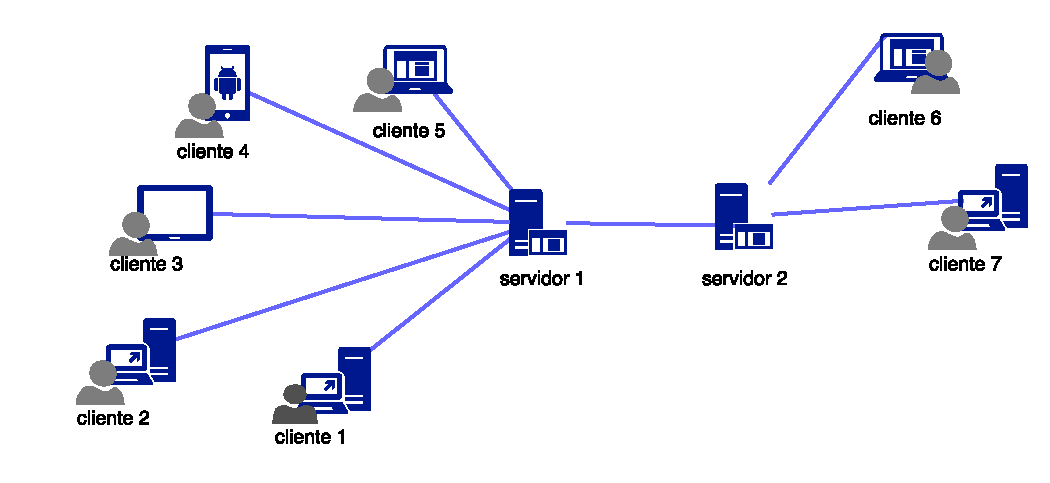
\includegraphics[width=0.6\textwidth]{clienteServidorP.pdf}
\captionsetup{justification=centering,margin=2cm}
\caption{Computaci'on cliente-servidor, adoptado para la realizac'ion del proyecto. Arquitectura cliente servidor de Somerville\cite{Somerville2011}}
\label{fig:clienteServidor}
\end{figure}

Para implementar un sistema cliente servidor tiene que instalar un programa en la computadora cliente para que se comunique con el servidor. Este cliente no tiene estado y no se implementa es como un conjunto de servicios independientes. Este cliente es conocido como SOA que se explica a continuaci'on.

\section{La arquitectura orientada a servicio web}
El arquitectura orientada a servicios es un componente de software de reutilizaci'on, debidamenta ajustado se accede de manera program'atica. \cite{Somerville2011}. Como se muestra en la figura \ref{fig:ArquitecturaSOA}.

\begin{figure}[H]
\centering
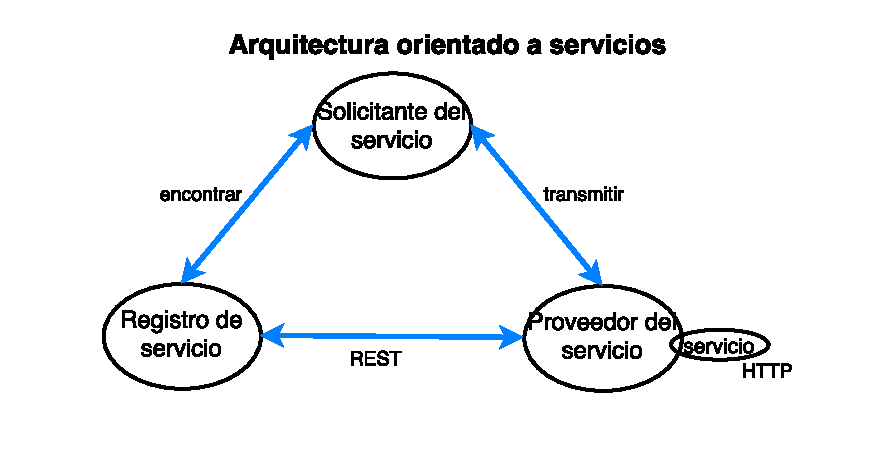
\includegraphics[width=0.4\textwidth]{arqSOA.pdf}
\captionsetup{justification=centering, margin=2cm}
\caption{Arquitectura orientado a servicio, adoptado para la realizac'ion del proyecto. El objetivo del SOA de Somerville \cite{Somerville2011}}
\label{fig:ArquitecturaSOA}
\end{figure}

Las caracter'isticas del servicio web son las siguientes:
\begin{enumerate}
\item Compartir informaci'on entre empresas.
\item La informaci'on debe tener una representaci'on est'andar.
\item Es indepediente de la aplicaci'on o sistema que usa el servicio web.
\item El servicio web es independiente de la plataforma y del lenguaje de implementaci'on.
\item Desde el principio, tiene un proceso est'andar para el servicio web en donde las compa'nias se han comprometido a dicho est'andar. 
\end{enumerate}

%Para el presente proyecto la implementaci'on y la interface del servicio, son definidos como un sistema heredado.

%\subsection{Sistema heredado}
%El sistema heredado es un sistema de software antiguo, donde es posible acceder a la funcionalidad del sistema mediante una nueva aplicaci'on que brinde acceso a las funciones y datos de un sistema heredado y utilizar nuevas tecnolog'ias\cite{Somerville2011}. Como se muestra en la figura \ref{fig:heredado}.

%\begin{figure}[H]
%\centering
%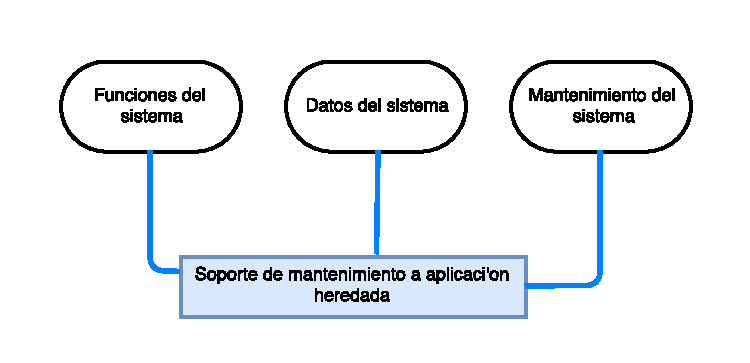
\includegraphics[width=0.5\textwidth]{servicioHeredado.pdf}
%\captionsetup{justification=centering, margin=2cm}
%\caption{Servicio heredado, adoptado para la realizac'ion del proyecto. Representaci'on de un servicio heredado de \cite{Somerville2011}}
%\label{fig:heredado}
%\end{figure}

La uni'on y la comunicaci'on entre el cliente y el servicio se realiza mediante diferentes  protocolos que se explicara continuaci'on.

\subsection{Protocolo de servicio}
El protocolo de servicio es un conjunto de reglas que se utilizan para la comunicaci'on e intercambio de informac'ion entre el protocolo mencionado anteriormente y a tr'aves de una red (Navarro, 2006).\cite{Navarro2006}. 
Seg'un Navarro los protocolos se dividen en dos tipos:
\begin{itemize}
\item Protocolos est'andares son : SOAP, WSDL \footnote{WSDL - Descripcion de lenguajes de servicios web}, WS-BPEL \footnote{WS-BPEL - Lenguaje de Ejecuci'on de procesos de negocio con servicios web}.
\item Protocolo no est'andar: el metodo REST.
\end{itemize}
 
Para el presente proyecto se ha utilizado el protocolo  REST se desarrolla en el siguiente parr'afo.

\section{Protocolo REST} 
El protocolo REST es un estilo de arquitectura de software que se refiere a una colecci'on de principios para el dise'no de arquitecturas en la red. El t'ermino frecuentemente es utilizado en el sentido de describir a cualquier interfaz que transmite datos espec'ificos de un dominio sobre HTTP\footnote{ HTTP- Hipertexto de Transferencia de Protocolo}. Se basa en est'andares de protocolo HTTP(Navarro, 2006).\cite{Navarro2006}.

\subsection{Protocolo HTTP}

El protoco HTTP es un conjunto de m'etodos de petici'on para indicar la acci'on que se desea realizar, en el recurso determinado cada uno de ellos implementan una sem'antica diferente, pero tienen alguna caracter'istica similar, las cuales son: Get, Head, Post, Put, Delete, Connect, Options, Trace y Patch.(Navarro, 2006) \cite{Navarro2006}. 

Seg'un Navarro, las funciones sobre la web que maneja HTTP son: el cache, los requisitos de origen,el proxie, el t'unel y sesi'on. \\

A continuaci'on se describen las funciones que se exploran en este proyecto.
\begin{enumerate}
\item \textbf{El cache:} es la funci'on para almacenar los documentos en la memoria del navegador. 
\item \textbf{ Requisitos de origen:} son funci'ones para compartir la informaci'on de datos y puede flexibilizar la informaci'on entre cliente y servidor. 
\item \textbf{La autentificaci'on:} es la funci'on que establece la sesi'on y almacena informaci'on en el cokie para guardar en el navegador. 
\end{enumerate}

\section{Unidad de datos del servicio}
La unidad de datos del servicio es un termino gen'erico para compartir informaci'on entre el servicio y el cliente. Estas unidades de datos pueden ser: Json\footnote{Json- Notaci'on de objetos de javascript}, Xml\footnote{XML-Lenguaje de Marcado Extensible} y Yaml \footnote{Yaml-Otro lenguaje de marcado m'as}. La unidad de datos Json se ha empleado en este proyecto se explica a continuaci'on.

\subsection{Json}
El Json es un formato ligero y abierto de intercambio de datos. Utiliza  el texto plano para compartir informaci'on, el c'ual es  independiente del lenguaje de programaci'on.  
Las estructura para compartir informaci'on pueden ser objetos o arreglo y tambi'en se puede combinar ambos, como se muestran en la figura \ref{fig:jsonO} y \ref{fig:jsonA} a continuaci'on.

\begin{figure}[H]
\begin{minipage}{0.48\textwidth}
\centering
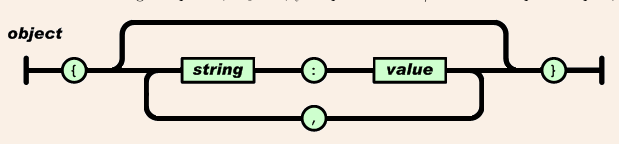
\includegraphics[width=0.8\textwidth]{jsonObj.png}
\captionsetup{justification=centering,margin=2cm}
\caption{Representaci'on de json por objeto, adoptado para la realizaci'on del proyecto. Estructura de json por objeto, de Figura: Elaboraci'on propia}
\label{fig:jsonO}
\end{minipage}\hfill
\begin {minipage}{0.48\textwidth}
\centering
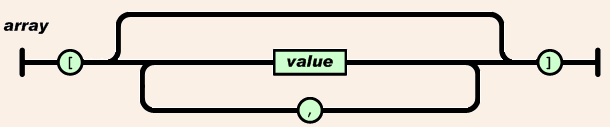
\includegraphics[width=0.8\textwidth]{jsonArr.png}
\captionsetup{justification=centering,margin=2cm}
\caption{Representaci'on del json por arreglo, adoptado para la realizaci'on del proyecto. Estructura de json por arreglo de Fuente: Elaboraci'on propia}
\label{fig:jsonA}
\end{minipage}
\end{figure}

\subsection{Json web token}
El json web token conocico como JWT\footnote{JWT - Json web token} es un m'etodo abierto y est'andar para representar las  solicitudes de forma segura entre dos partes. Este se dividen tres partes: la cabecera, la carga 'util y una firma.

\begin{figure}[H]
\centering
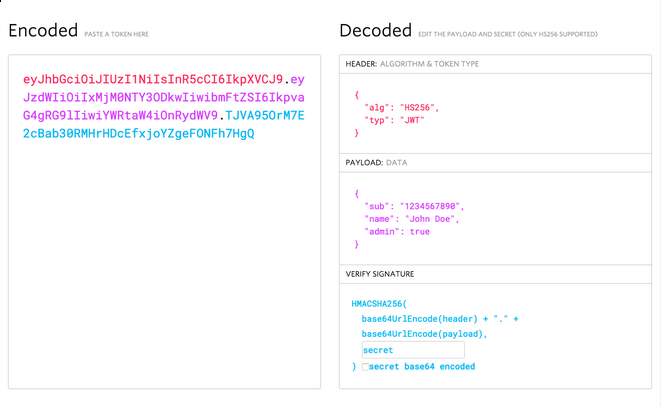
\includegraphics[width=0.6\textwidth]{arqJWT.png}
\captionsetup{justification=centering,margin=2cm}
\caption{ Representaci'on del json web token Fuente: Elaboraci'on propia}
\end{figure}

En este proyecto el tipo de servicio web es identificado como un servicio heredado porque realiza solicitud de datos para la aplicaci'on m'ovil.

\section{Las aplicaciones m'oviles}
Seg'un la corporaci'on de IBM \footnote{IBM - M'aquinas de negocios internacionale}  define a las aplicaciones m'oviles en tres partes, las cuales son: nativa, web y hibrido. \cite{Ibm2012}

\subsection{La aplicaci'on nativa}
La aplicaci'on nativa se conecta directamente con el sistema operativo m'ovil, sin ning'un intermediario ni contenedor. La aplicaci'on nativa puede acceder libremente a todas las Apis que el proveedor del sistema operativo ponga a su disposici'on y en muchos casos, tiene caracter'isticas y funciones 'unicas que son t'ipicas del sistema operativo m'ovil en particular.
%Nos hemos quedado aqui
\subsection{La aplicaci'on web}
La aplicacion web utiliza 'unicamente tecnolog'ias basadas en la web como ser la quinta version de HTML \footnote{HTML - Lenguaje de Marcado para Hipertexto}, el mismo tiene componente de interfaz de usuario avanzado, acceso a m'ultiples tipos de medios, servicios de geoposicionamiento y disponibilidad sin Internet.\\
Una ventaja de esta aplicaci'on es el soporte para m'ultiples plataformas y se ejecuta dentro del navegador.
\subsection{La aplicaci'on h'ibrida}
La aplicaci'on h'ibrida tiene un  enfoque h'ibrido que combina desarrollo nativo con tecnolog'ia web. La aplicaci'on hibrida utiliza  m'ultiples plataformas y tiene acceso a los dispositivos del celular tales son: la camara, acceso de dato, almacenamiento de informaci'on y otros.

En este proyecto se ha utilizado la aplicacion h'ibrida porque permite acceder a la parte nativa del m'ovil y almacena informaci'on en la aplicaci'on.

\section{Los dispositivos m'oviles}
Actualment'e, el dispositivo m'ovil es peque'no para ser manejado facilmente se ha utilizado durante su transporte. Se caracteriza por el mejoramiento que va adquiriendo su tama'no reducido, la telecomunicaci'on de software,  la gran iteracci'on entre las personas. Convirt'iendolos en una necesidad primaria para la sociedad\cite{Morillo2014}.\\
Desde su creaci'on  los dispositivos m'oviles han evolucionado en gran magnitud, es por eso que muchas empresas han ofrecido diferentes sistemas operativos como ser: android, ioS, Windows, etc. El sistema operativo de android se utiliza para el presente proyecto.

\subsection{El sistema operativo android}
E sistema operativo android basada en la  plataforma de software Linux para dispositivos m'oviles. 
El sistema operativo android es un sistema operativo libre y tiene acceso a sus recursos como la pantalla, camara y otros\cite{Android}. A continuaci'on consta con las siguientes capas, se muestra en la siguiente figura \ref{fig:Android}.

\begin{figure}[H]
\centering
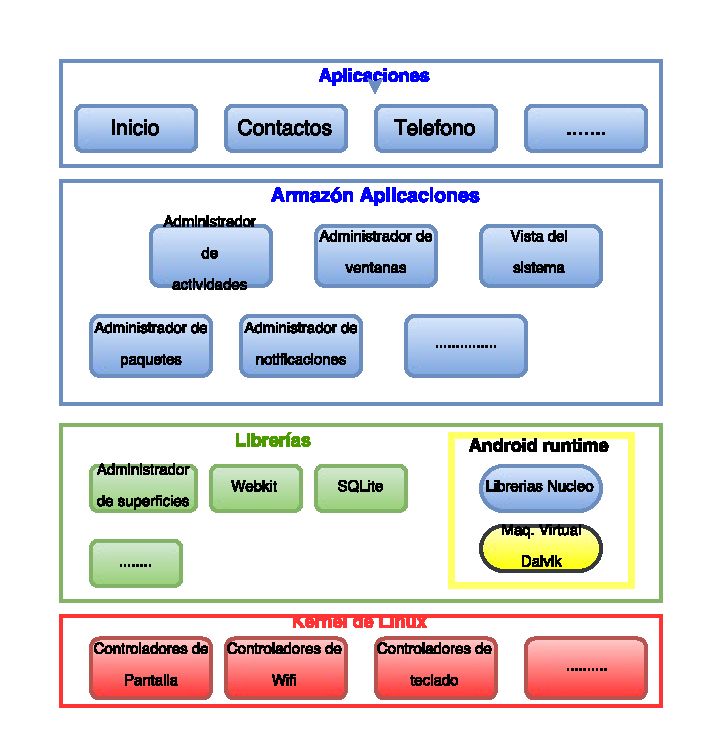
\includegraphics[width=0.3\textwidth]{capaAndroid.pdf}
\captionsetup{justification=centering, margin=2cm}
\caption{Capas del sistema operativo de android, adoptado para la realizac'ion del proyecto. Fuente: Introducci'on a Android  \cite{Android}}
\label{fig:Android}
\end{figure}

Con el avance de la tecnolog'ia han aumentado el incremento, en diferentes dispositivos como ser tablet PC, tablet, smartphone y otros el c'ual utilizan el sistema operativo android. 
%Debido a la diversidad de dispositivos m'oviles, para el presente proyecto se utiliza el dise'no adaptativo que se explica a continuaci'on.

%\section{El dise'no adaptativo}
%El dise'no adaptativo se refiere a la satisfacci'on de visitar una p'agina web a tr'aves de diferentes dispositivos, ha  generado la filosof'ia de  Responsive Web Design, este pensamiento fue establecida por Steven Champeon (2003), qui'en propone realizar un 'unico dise'no web para todos los dispositivos y accesible para todos los usuarios \cite{Adrian2012}.

\section{Las herramientas para las plataformas de desarrollo}
Las herramientas  para el desarrollo las cuales son: 'el entorno de desarrollo vim y 'el navegador de chrome.

\subsection{El entorno de desarrollo VIM}
Seg'un la p'agina oficial de Vim, el Vim se define como un editor de texto altamente configurable construido para creaciones y cambios de cualquier tipo de texto. Tiene las siguientes ventajas: persistente multinivel, extensivos plugin para el sistema, soportan diferentes lenguajes de programaci'on y diferentes formatos de archivos y otros.
\subsection{El navegador web - Chrome}
Es un navegador web r'apido, seguro y gratuito, dise'nado para la web actual, as'i lo define la p'agina oficial del mismo.
 
Tambi'en es un navegador para dispositivos m'oviles.  La ventaja que brinda es verificar los errores para celulares, minimizar los gastos de datos, almacenar la sesi'on y permitir crear base datos en el navegador.

\section{Herramientas de desarrollo}
Se utilizo tres framework los cuales son ionic, angularjs y nodejs. Estos se basan en el lenguaje de javaScript para la implementaci'on del servicio web y la aplicaci'on  m'ovil las cuales son:

\subsection{Framework ionic}
Seg'un la p'agina oficial de  ionic este framework es un SDK para HTML5 que nos ayuda a construir una aplicaci'on m'ovil h'ibrida usando las tecnolog'ias como HTML, CSS y Javascript. Se caracteriza por ser multiplataforma y utiliza el framework de angularJS.

\subsection{Framework angularJS}
Seg'un la p'agina oficial de angularJS este es un conjunto de  herramientas  para construir el framework  mas adecuado para desarrollo de aplicaciones. Es totalmente extensible y trabaja con otras librer'ias, cada caracter'istica puede ser modificado o remplazado, para adaptarse a su  flujo de trabajo.

\subsection{Framework node.js}
El framework de nodeJS es un entorno de ejecuci'on para javaScript construido con el motor JavaScript V8 de Chrome. Nodejs utiliza un modelo de operaci'on de E/S sin bloqueo y orientado a eventos que lo hace liviano y eficiente. El ecosistema de paquetes de Node.js, npm, es el ecosistema mas grande de librer'ias de c'odigo abierto en el mundo. Seg'un la p'agina oficial de nodejs.
%aumentado
Para el desarrollo de la aplicaci'on m'ovil se ha utilizado el framework ionic.
Ionic es de c'odigo libre y se basa en librer'ias orientadas 'unicamente a aplicaciones de dispositivos m'oviles. Tambi'en se enfocan a desarrollo de aplicaciones h'ibridas construida con HTML3, CSS3 y Javascript se construye p'aginas web, se ejecutan dentro de un navegador, el c'ual aportan para ejecutar, en diferentes plataformas: android, iOS, windowsPhone, etc. Utiliza el framework de angular y es integrado con cordova el c'ual permite el acceso a las caracter'isticas nativas del dispositivo.El framework de angular ha  utilizado la arquitectura de patrones de modelo, vistas y controladores es la base para la arquitectura de ionic, se muestra en la figura \ref{fig:Ionic}.

%figura Arquitectura de Ionic
\begin{figure}[H]
\centering
 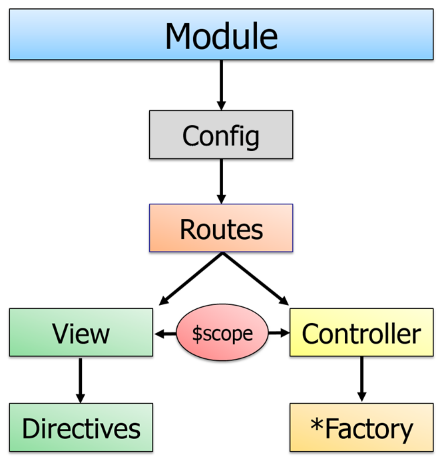
\includegraphics[width=0.5\textwidth]{arqIonic.png}
 \captionsetup{justification=centering,margin=2cm}
 \caption{Arquitectura de Ionic, adoptado para la realizac'ion del proyecto Fuente: Introducci'on a ionic\cite{Gallego}}
\label{fig:Ionic}
\end{figure}

\section{Herramientas extras}
Para el presente proyecto se ha utilizado algunas herramientas extras como ser: cordova, pouchDB, json web token y localstorage.

\subsection{Framework cordova}
Cordova es un framework de c'odigo libre para desarrollo m'ovil que nos permite usar est'andares de tecnolog'ias web como HTML5,CSS3 y Javascript. Se basa en los enlaces de API's compatibles para acceder a las capacidades del dispositivos como sensores, red, etc. En la figura \ref{fig:arqCordova} se muestra arquitectura de Cordova.

\begin{figure}[H]
\centering
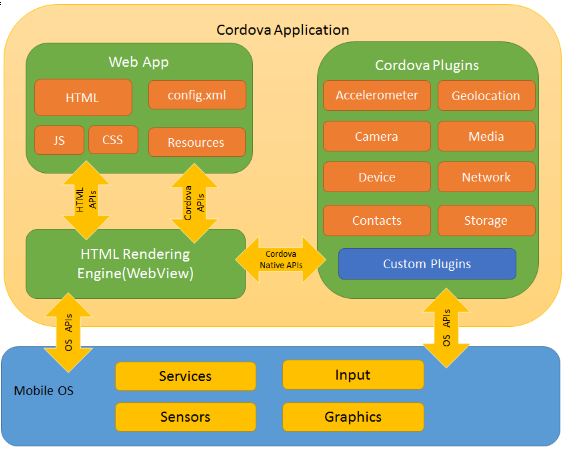
\includegraphics[width=0.3\textwidth]{arqCord.png}
\captionsetup{justification=centering,margin=2cm}
\caption{Arquitectura de cordova, adoptado para la realizac'ion del proyecto Fuente: Arquitectura de cordova\cite{Cantabriatic}}
\label{fig:arqCordova}
\end{figure}

Para el presente proyecto se utiliza cordova y se agrega su librer'ia al proyecto despu'es se instalan los plugins necesarios.

\subsection{PouchDB}
PouchDb es una capa de otras base de datos y se almacenan en el navegador esto permite guardar los datos a lado del cliente y se implementa en el lenguaje de JavaScript. La estructura de pouchdb se representa en la siguiente figura \ref{fig:pouchDB}.\cite{Pouch} 
\begin{figure}[H]
\centering
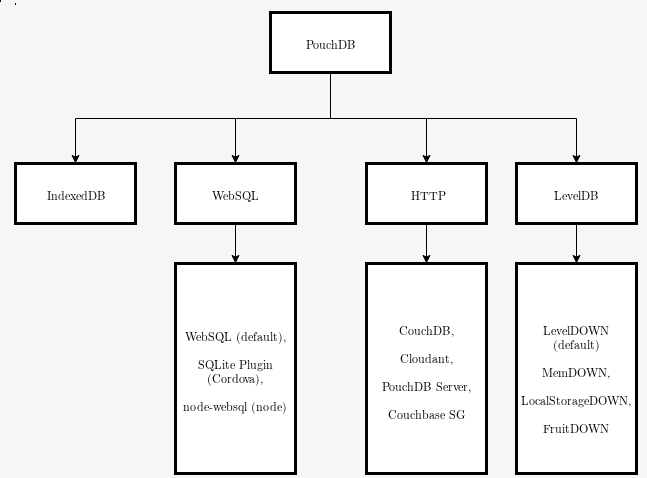
\includegraphics[width=0.3\textwidth]{pouchDB.png}
\captionsetup{justification=centering,margin=2cm}
\caption{Adaptadores de PouchDB, adoptado para la realizac'ion del proyecto Fuente: Antecedente de pouchdb\cite{Pouch}}
\label{fig:pouchDB}
\end{figure}

Seg'un la p'agina oficial de pouchDB es una base de datos NoSQL. El uso de esta API, podemos construir aplicaciones que funcionan fuera de sin conexi'on a internet y con conexi'on a internet. PouchDB utiliza WebSQL y IndexedDB internamente para almacenar los datos. 

%Para el presente proyecto se ha utilizado la capa del adaptador de websql, se explica a continuaci'on.

\subsection{Base de datos websql}
Es una herramienta para internet e intranets que facilita el acceso a base de datos relacionada con la web. Integra la tecnolog'ia  del cliente y abre la sybase el c'ual permite que los datos de la fuente se incorporen din'amicamente en la p'agina web. En la siguiente figura \ref{fig:websql} se representa la base de datos websql.
\begin{figure}[H]
\centering
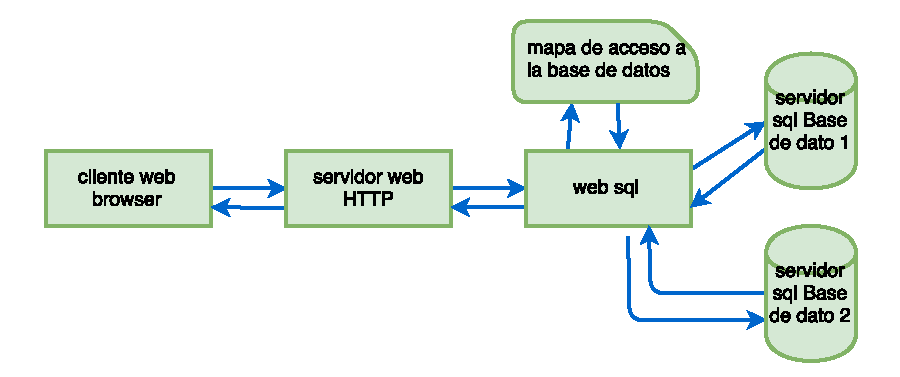
\includegraphics[width=0.6\textwidth]{websql.pdf}
\captionsetup{justification=centering,margin=2cm}
\caption{Base de datos websql, adoptado para la realizac'ion del proyecto Fuente: Adaptador de websql \cite{Websql1997}}
\label{fig:websql}
\end{figure}

\subsection{Almacenamiento local}
Es una propiedad de HTML5 web de almacenamiento, que permiten almacenar datos en nuestro navegador web denominada localstorage.
Guarda la informaci'on que permanece almacenada por tiempo indefinido, sin importar que el navegador se cierre. Tiene las siguientes caracteristicas, almacenar entre 5MB y 10MB de informaci'on, est'a almacenada en la computadora del cliente y no es enviado en cada petici'on del servidor, previene perdidas de informaci'on cuando se desconecta de la red y la informaci'on es guardada por dominio web \cite{Cardenas2015}.
\subsection{Interceptor}                                                                                                                                                                                                                                              
El interceptor utiliza el servicio de \textit{http} el c'ual permite la comunicaci'on con el servidor y captura cada petici'on y lo manipula a trav'es del \textit{httpProvider} es el que registra el contenedor del arreglos y ofrece un servicio regulador.
\subsection{Json web token}
Json web token es un m'etodo abierto y est'andar para representar las  reclamaciones de forma segura, entre dos partes que comparten informaci'on y autentificaci'on moderna, de m'ovil. El c'ual tiene una estructura representada en la figura \ref{fig:jwt}.
\begin{figure}[H]
\centering
\includegraphics[width=0.6\textwidth]{jwt.pdf}
\captionsetup{justification=centering,margin=2cm}
\caption{Json web token, adoptado para la realizac'ion del proyecto Fuente: Elaboraci'on propia}
\label{fig:jwt}
\end{figure}

Estos son las herramientas extras como se han mencionado anteriormente estas se utilizan para el presente proyecto los c'uales son compatibles con el framework ionic. 
\chapter{An'alisis de la planilla de notas}
\label{capitulotres}
El plantel docente de la Facultad de Ciencias y Tecnolog'ia de la Universidad Mayor de San Sim'on utiliza la p'agina del Sistema de Apoyo a la Gesti'on Acad'emica y Administrativa el c'ual tiene una secuencia de pasos  para descargar y publicar la planilla de notas. Para reconocer y modificar la planilla de notas se utiliza, la aplicaci'on del transcriptor.exe la  c'ual tiene diferentes casos, dependiendo de la estructura de la planilla de notas.

\section{Entrevista}
La siguiente entrevista se realizo al \textit{Ing. Cristian Lazarte}, responsable del proyecto Transcriptor.exe en la UPSI \footnote{UPSI-Unidad de Provisi'on de Servicios de Informaci'on} de la UMSS \footnote{UMSS-Universidad Mayor de San Sim'on}. A continuaci'on se muestra los resultados de la entrevista en los siguientes puntos.
\begin{itemize}
\item Explicaci'on de la estructura de planilla de notas, el archivo sis:
\begin{itemize}
\item El c'odigo de la UPSI.
\item El c'odigo de template define la estructura que utiliza el Transcriptor.exe.
\item En el template el ARB son valores permitidos, para A de aprobado, R reprobado y B abandonado.
\item Los datos del grupo est'an definidos en el template y las restricciones de las calificaciones.
\end{itemize}
 
\item Mencionamos  algunos de los aspectos importantes y/o limite que considera a la hora de modificar la planilla de notas en el transcriptor.exe.
\begin{itemize}
\item Modificar las notas se debe mostrar en grillas.
\item Los estados para volver atras.
\item Cuando modifica la lista de estudiantes, no debe permitir cerrar sin guardar.
\item Habilitar la 2da opci'on y tomar en cuenta el mayor entre la 1ra y 2da opci'on.
\item En el enter, ir al siguiente dato para introducir.
\item Analizar la visualizaci'on en el dispositivo m'ovil.
\end{itemize}
\end{itemize}
La entrevista ha proporcionado la comprensi'on  de la estructura y la funcionalidad al modificar la planilla de notas.

\section{Diagrama de proceso de llenar la planilla de notas}
Los procesos de llenar la planilla de notas tiene los siguientes pasos:  descargar la planilla de notas, modificar la planilla de notas y adjuntar la planilla de notas. Se explica con mas detalle en el c'apitulo \ref{capitulocinco} en la secci'on de \ref{Doc:Interfaz}.\\ 
La uni'on de los proceso se representa en un diagrama general como se muestra en la  figura \ref{fig:DiagramaF}
\begin{figure}[H]
\centering
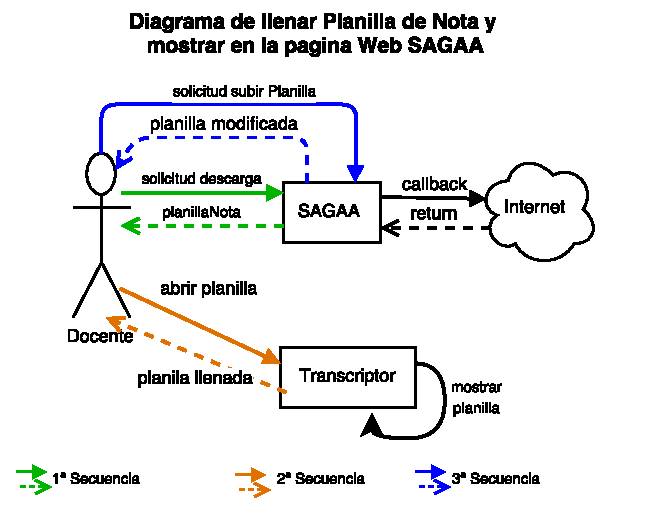
\includegraphics[width=0.4\textwidth]{SGeneralLlenaN.pdf}
\captionsetup{justification=centering, margin=2cm}
\caption{Diagrama de la funcionalidad de llenar y mostrar las notas, en la p'agina del SAGAA Fuente: Elaboraci'on propia}
\label{fig:DiagramaF}
\end{figure}

A continuaci'on se explica la funcionalidad del llenado de planilla de notas de la p'agina SAGAA\footnote{SAGAA-Sistema de Apoyo a la Gesti'on Acad'emica y Administrativa} y la herramienta del transcriptor.exe.


\section{Sistema de apoyo a la gesti'on acad'emica y administrativa}
El sistema de apoyo a la gesti'on acad'emica y administrativa tiene alrededor de 10 a'nos proporcionando el servicio de gestionar la informaci'on acad'emica de pre-grado de los estudiantes.

La funcionalidad de la informaci'on acad'emico de pre-grado tiene los siguientes procesos: 
\begin{itemize}
\item Llenar curriculum.
\item Publicar y modificar avisos.
\item Publicar y modificar las materias.
\item Descargar la planilla de notas.
\item Habilitar la planilla de notas.
\item Ver estudiantes habilitados.
\item Administrador de archivos y manual.
\end{itemize}


Para el presente proyecto se ha utilizado la funcionalidad de modificar la planilla de notas: descargar y habilitar la planilla de notas. Las cuales son.

\subsection{Funcionalidad de modificar la planilla de notas}
La funcionalidad de modificar la planilla de notas tiene los siguientes procesos  descargar, modificar y adjuntar la planilla de notas. A continuaci'on se explican. 

\subsection{Los pasos para descargar la planilla de notas}
\label{PasosDescargar}
Para realizar la descarga de la planilla de notas se explican en los siguientes pasos:
\begin{enumerate}[\bfseries P{a}so 1:]
\item Primeramente, se debe escribir la direcci'on de la p'agina en el navegador: \url{http://pruebas.fcyt.umss.edu.bo/sagaa}. Despu'es se debe acceder al link \textbf{Ingresar al sistema}, debe ingresar su cuenta de usuario y contrase'na as'i como se muestra en la figura \ref{fig:Paso2P}.
%\begin{figure}[H]
%\centering
%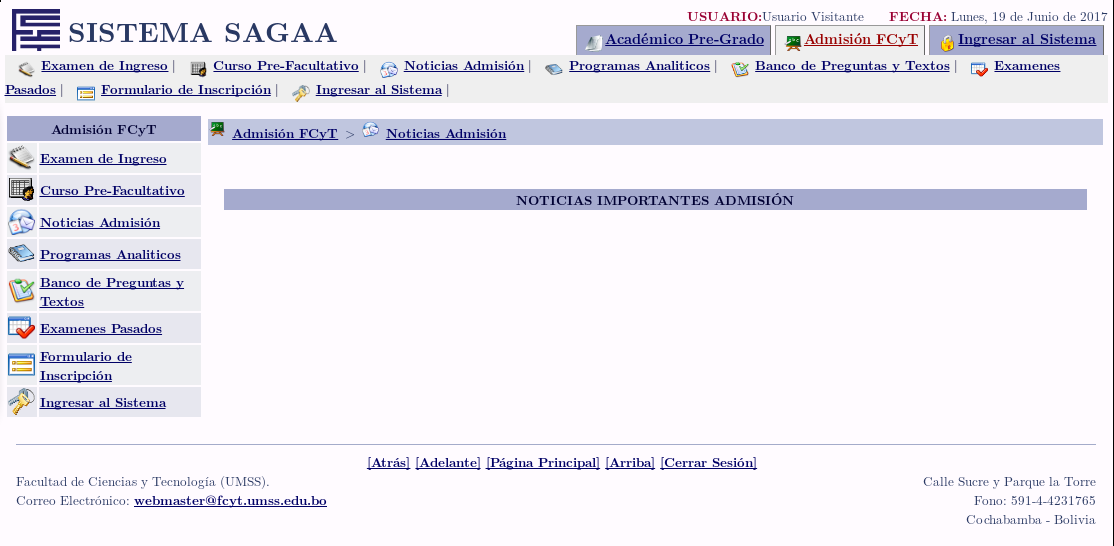
\includegraphics[width=0.5\textwidth]{pagS.png}
%\captionsetup{justification=centering, margin=2cm}
%\caption{Inicio de p'agina del SAGAA Fuente: Proporcionado por la UPSI de la FCYT}
%\label{fig:Paso1P}
%\end{figure}

%\item \textbf{Paso 2:} Hacer click en el link \textit{Ingresar al sistema}, debe ingresar su cuenta de usuario y contrase'na, se muestra en la figura \ref{fig:Paso2P}.
\begin{figure}[H]
\centering
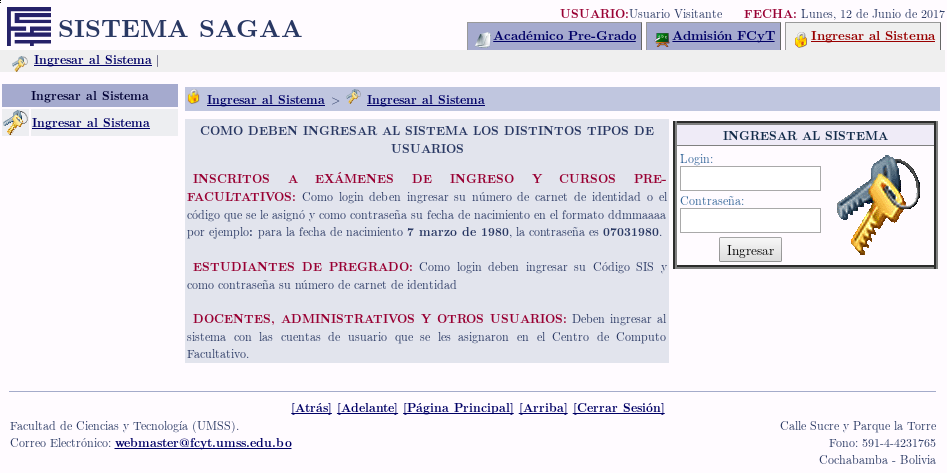
\includegraphics[width=0.5\textwidth]{pagS1.png}
\captionsetup{justification=centering, margin=2cm}
\caption{Iniciar sesi'on en la p'agina del SAGAA Fuente: Proporcionado por la UPSI de la FCYT}
\label{fig:Paso2P}
\end{figure}

\item Elegir el m'enu de usuario \textbf{Acad'emico Pre-Grado} en la figura \ref{fig:Paso3P}.
\begin{figure}[H]
\centering
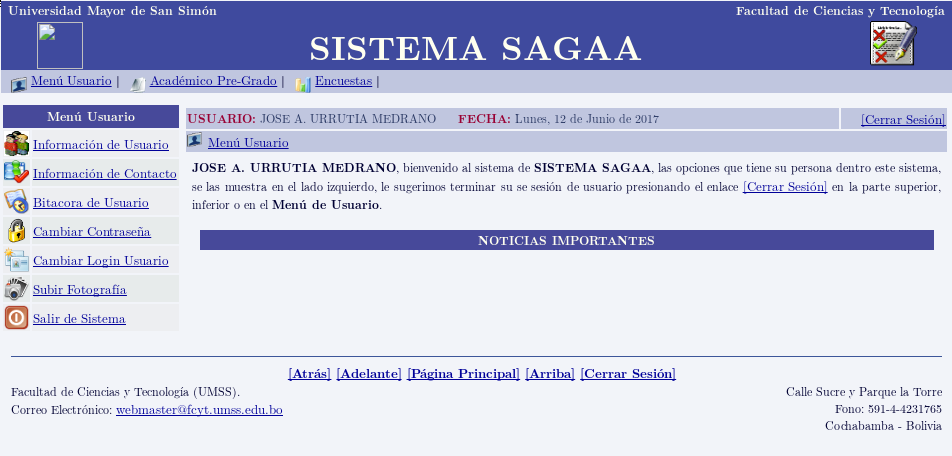
\includegraphics[width=0.5\textwidth]{pagS2.png}
\captionsetup{justification=centering, margin=2cm}
\caption {Elegir men'u Ac'ademico Pre-Grado Fuente: Proporcionado por la UPSI de la FCYT}
\label{fig:Paso3P}
\end{figure}

\item Elegir el men'u la opci'on \textit{" Descargar Planilla de Notas"} de  la figura \ref{fig:Paso4P}.
\begin{figure}[H]
\centering
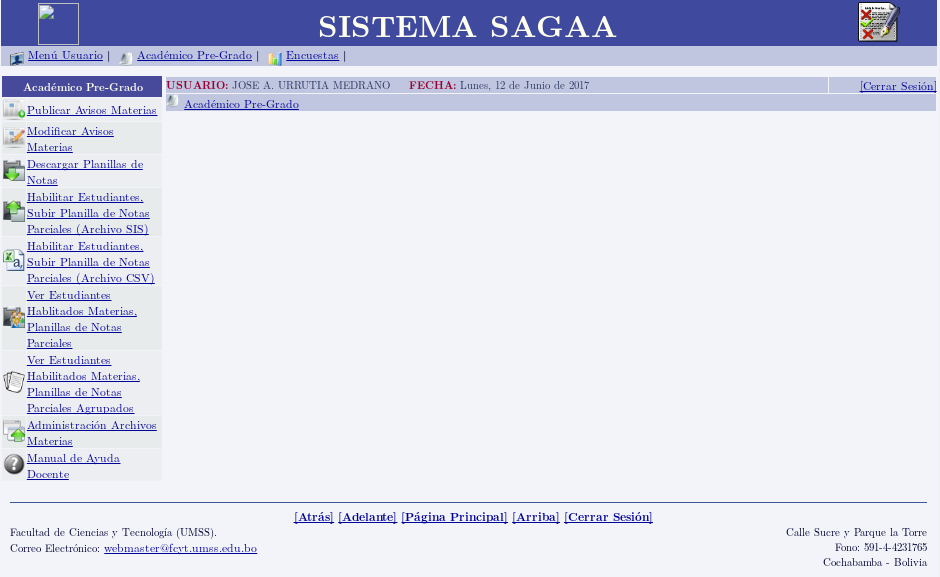
\includegraphics[width=0.5\textwidth]{pagS3.png}
\captionsetup{justification=centering, margin=2cm}
\caption{Elegir la opci'on descargar la planilla de notas Fuente: Proporcionado por la UPSI de la FCYT}
\label{fig:Paso4P}
\end{figure}

\item En la figura \ref{fig:Paso5P} se debe seleccionar la gesti'on de la lista de opciones \textbf{Seleccionar gesti'on}.
\begin{figure}[H]
\centering
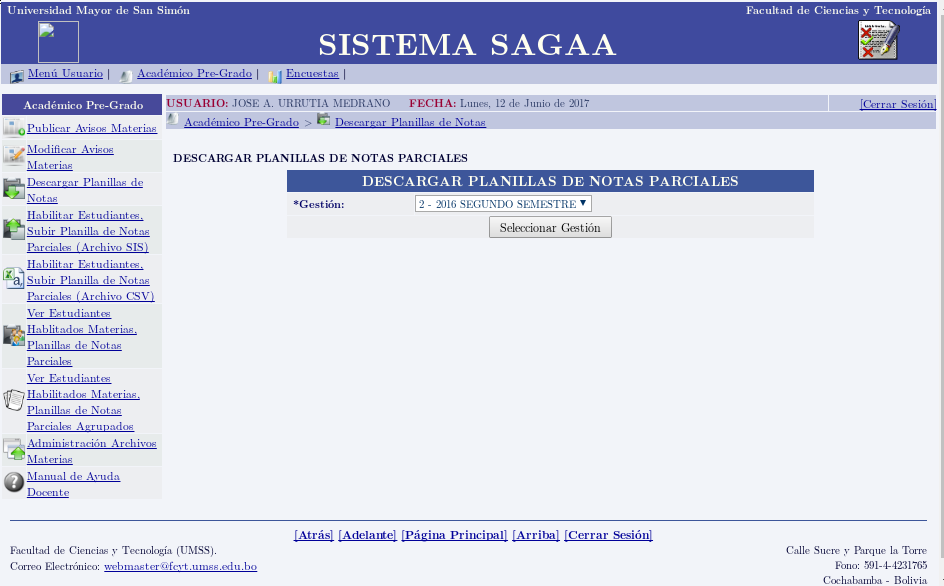
\includegraphics[width=0.5\textwidth]{pagS4.png}
\captionsetup{justification=centering, margin=2cm}
\caption{Opci'on de gesti'on, Fuente: Proporcionado por la UPSI de la FCYT}
\label{fig:Paso5P}
\end{figure}

\item Seleccionar el icono de descarga de la lista de carrera para \textit{Descargar la  planilla de notas}, como se muestra en la figura \ref{fig:Paso6P}.
\begin{figure}[H]
\centering
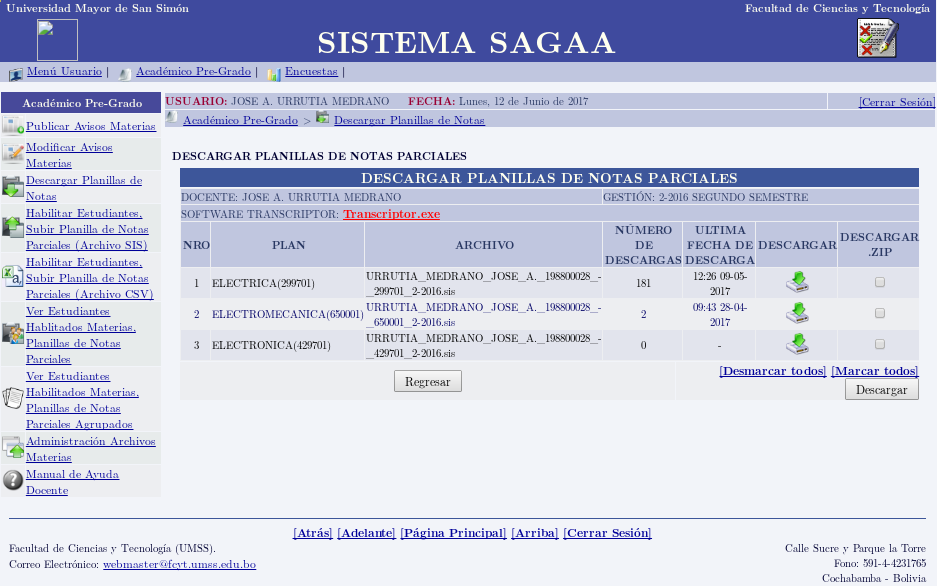
\includegraphics[width=0.5\textwidth]{pagS5.png}
\captionsetup{justification=centering, margin=2cm}
\caption{Elegir la descarga de una planilla de notas, Fuente: Proporcionado por la UPSI de la FCYT}
\label{fig:Paso6P}
\end{figure}
\end{enumerate}
Finalmente, el documento de planilla de notas debe llenar las notas y despu'es realizar el proceso de publicaci'on de la planilla de notas.

\subsection{Los pasos para publicar la planilla de notas}
Para publicar la planilla de notas, se realiza el paso 1 de \textbf{Ingressar al sistemas} y el paso 2 elegir el men'u \textbf{Acad'emico Pre-Grado} de la secci'on  \ref{PasosDescargar} de descargar la planilla de notas , despu'es se debe realizar los siguientes pasos:
\begin{enumerate}[\bfseries P{a}so 1:]
\item Elegir el men'u la opci'on, \textbf{Habilitar estudiantes, subir Planilla de Notas Parciales (Archivo SIS)}, como se muestra en la figura \ref{fig:Paso1PS}.
\begin{figure}[H]
\centering
\captionsetup{justification=centering, margin=2cm}
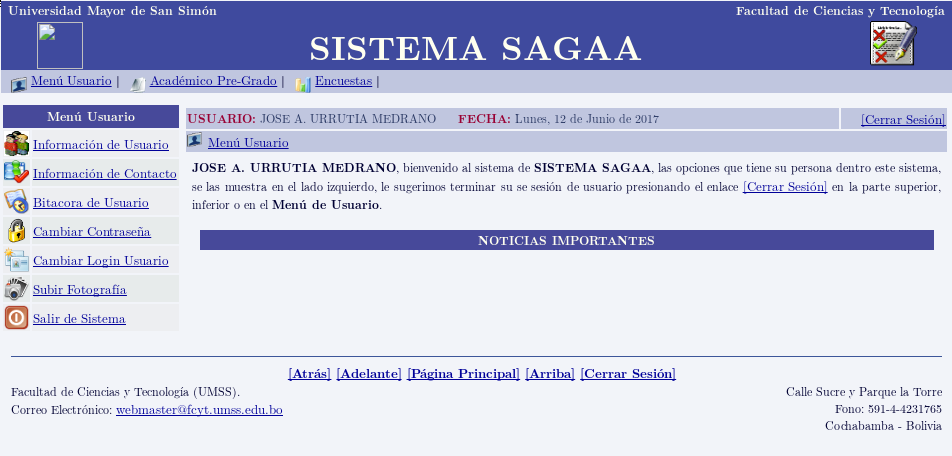
\includegraphics[width=0.6\textwidth]{pagS2.png}
\caption{Paso 1: Opci'on de habilitar estudiantes Fuente: Proporcionado por la UPSI de la FCYT}
\label{fig:Paso1PS}
\end{figure}

\item En la figura \ref{fig:Paso2PS} se adjunta el archivo y se selecciona la gesti'on de la lista de opciones, despu'es de hacer click en \textbf{Subir Archivo}
\begin{figure}[H]
\centering
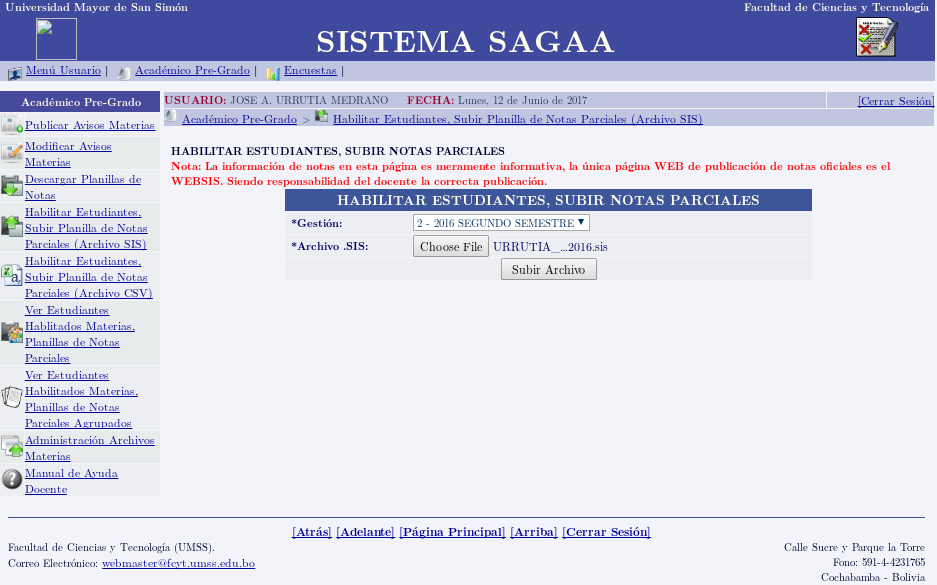
\includegraphics[width=0.5\textwidth]{pagS7.png}
\captionsetup{justification=centering, margin=2cm}
\caption{Paso 2: Opci'on de adjuntar el archivo seleccionado Fuente: Proporcionado por la UPSI de la FCYT}
\label{fig:Paso2PS}
\end{figure}

\item Seleccionar el grupo para adjuntar la planilla de notas y por ultimo click en \textbf{Finalizar Operaci'on} como se muestra en la figura\ref{fig:Paso3PS}.
\begin{figure}[H]
\centering
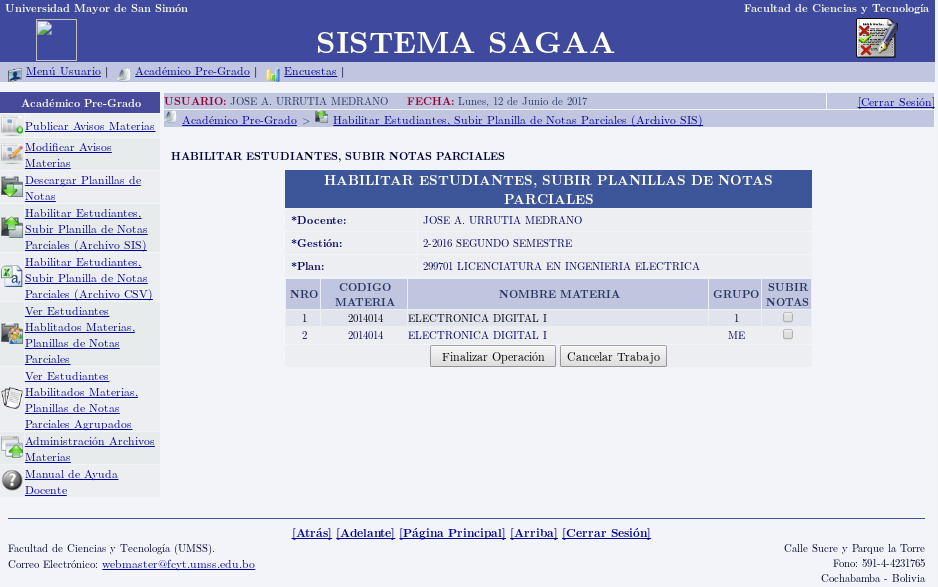
\includegraphics[width=0.5\textwidth]{pagS8.png}
\captionsetup{justification=centering, margin=2cm}
\caption{Paso 3: Subir planilla de notas por grupo Fuente: Proporcionado por la UPSI de la FCYT}
\label{fig:Paso3PS}
\end{figure}
\end{enumerate}

Al finalizar, se muestra el mensaje \textit{Finalizo la  habilitaci'on de estudiantes y la planilla de notas} y accede nuevamente al paso 1.

\subsection{Las restricciones de la p'agina del SAGAA}
Para concluir con el an'alisis de la p'agina del SAGAA se debe tomar en cuenta las siguientes restricciones: 
\begin{enumerate}
\item Solo permite subir planilla de notas con extensi'on sis.
\item Se debe estar conectado a internet para realizar el adjuntar o descargar la planilla de notas.
\end{enumerate}

\section{El transcriptor}
El trascriptor es un programa ejecutable tiene la funcionalidad de modificar la planilla de notas. Previamente, se descarga el documento de planilla de notas de la p'agina del SAGAA \footnote{SAGAA-Sistema de Apoyo a la Gesti'on Acad'emica y Administrativa}. El creador el  Lic. Cristian Lazarte,  qui'en actualmente trabaja en la UPSI \footnote{UPSI-Unidad de Provisi'on de Servicios de Informaci'on} realizando mantenimiento a dicha aplicaci'on.


\subsection{La funcionalidad de la aplicaci'on del transcriptor}
La funcionalidad del transcriptor es llenar la planilla de notas las cuales se describen en los siguientes pasos.
\begin{enumerate}[\bfseries P{a}so 1:]
\item Primeramente seleccionar el bot'on \textbf{Abrir} como se observa en el c'irculo azul. En segundo lugar se busca la ubicaci'on de la planilla de notas, como se observa en la figura \ref{fig:Paso1T}.
\begin{figure}[H]
\centering
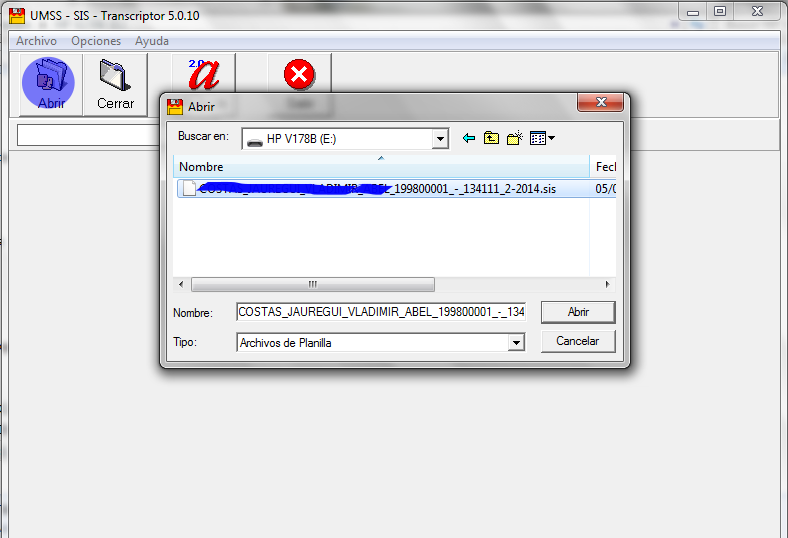
\includegraphics[width=0.5\textwidth]{t1.png}
\captionsetup{justification=centering, margin=2cm}
\caption{Buscar planilla de notas  del Transcriptor Fuente: Proporcionado por el MEMI}
\label{fig:Paso1T}
\end{figure}

\item Seleccionar un grupo y hacer click en el c'irculo azul, en el bot'on \textbf{Editar}, se representa en la figura \ref{fig:Paso2T}.
\begin{figure}[H]
\centering
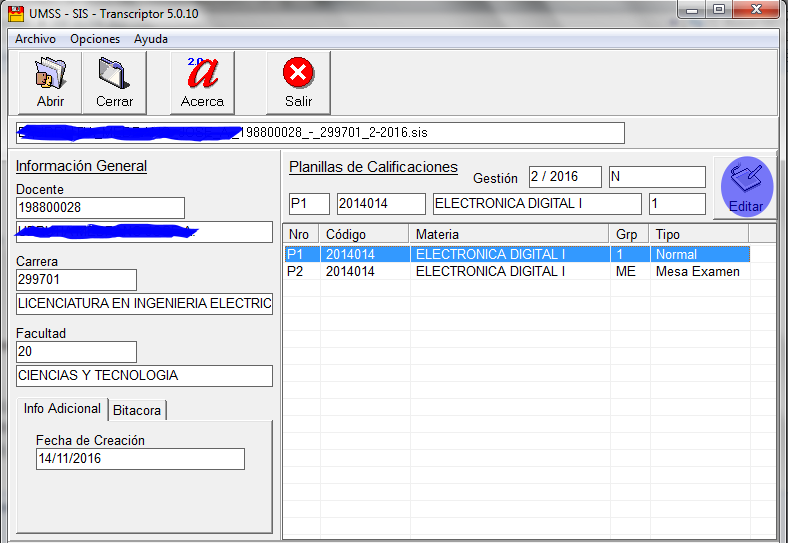
\includegraphics[width=0.5\textwidth]{t2.png}
\captionsetup{justification=centering,margin=2cm}
\caption{Buscar planilla de notas Fuente: Proporcionado por el MEMI}
\label{fig:Paso2T}
\end{figure}

\item En el c'irculo rosado se debe llenar las notas de forma ordenada, como se tiene en la figura \ref{fig:Paso3T}.
\begin{figure}[H]
\centering
\captionsetup{justification=centering,margin=2cm}
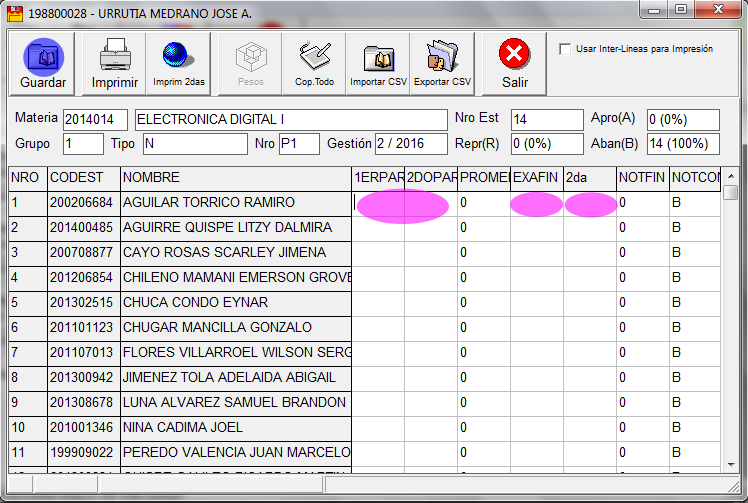
\includegraphics[width=0.6\textwidth]{t3.png}
\caption{Lista de estudiantes, Fuente: Proporcionado por el MEMI}
\label{fig:Paso3T}
\end{figure}
 
\item Guardar la planilla de notas y hacer click en el bot'on \textbf{Guardar} para cerrar la ventana y guardar los datos en el archivo de planilla de notas como se muestra en la figura \ref{fig:Paso3T}.
\end{enumerate}

Desp'ues de concluir con descargar y  adjuntar la planilla de notas, se modifica la planilla de notas con el transcriptor.exe.

\subsection{Detalle del Transcriptor}
El transcriptor interpreta los datos de la planilla de notas que se encuentra con la extensi'on sis, como se muestra en los siguiente casos a continuacio'on en la figura \ref{fig:Caso1T}.
\begin{enumerate}[\bfseries P{a}so 1:]
\item Mostrar los datos de la informaci'on general y la lista de materias, como se muestra en la figura \ref{fig:Caso1T}
\begin{figure}[H]
\centering
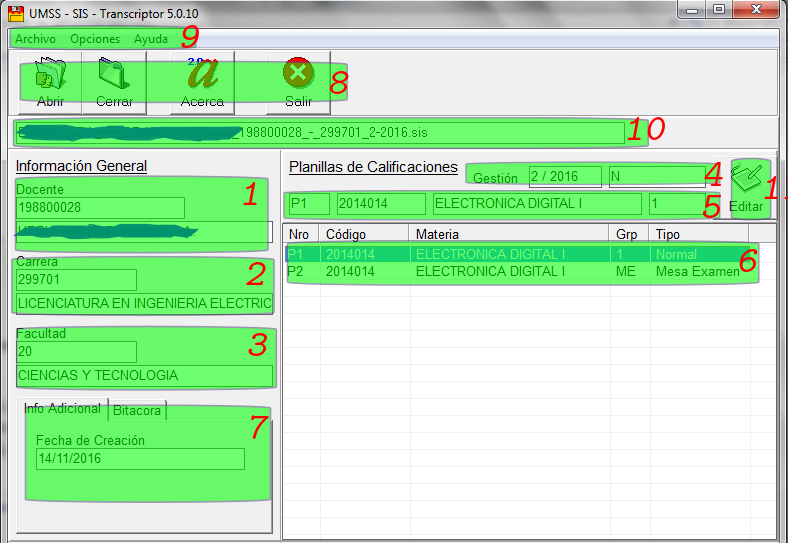
\includegraphics[width=0.6\textwidth]{td2.png}
\captionsetup{justification=centering,margin=2cm}
\caption{Detalle de la lista de grupo Fuente: Proporcionado por el MEMI}
\label{fig:Caso1T}
\end{figure}

Se divide en las siguientes partes, las cuales est'an enumeradas seg'un el detalle:
\begin{enumerate}
\item Los datos del docente: el c'odigo, el nombre y apellido.
\item Los datos de la carrera: el c'odigo y nombre.
\item Los datos de la facultad: el c'odigo y nombre.
\item El dato de la gesti'on.
\item Los datos del grupo: el c'odigo, nombre, c'odigo de reconocimiento y n'umero de grupo.
\item La lista de grupo: el n'umero, c'odigo, nombre, identificador y tipo.
\item La informaci'on adicional de una bitacora de la fecha de creaci'on y bit'acora del archivo.
\item En el men'u del n'umero 8 tiene los eventos  los cuales son: abrir, cerrar, acerca y salir.
\item En el men'u del n'umero 9 consta de los eventos: archivo, opciones y ayuda.
\end{enumerate}

\item Mostrar la lista de estudiantes, como se muestra en la figura \ref{fig:Caso2T}.
\begin{figure}[H]
\centering
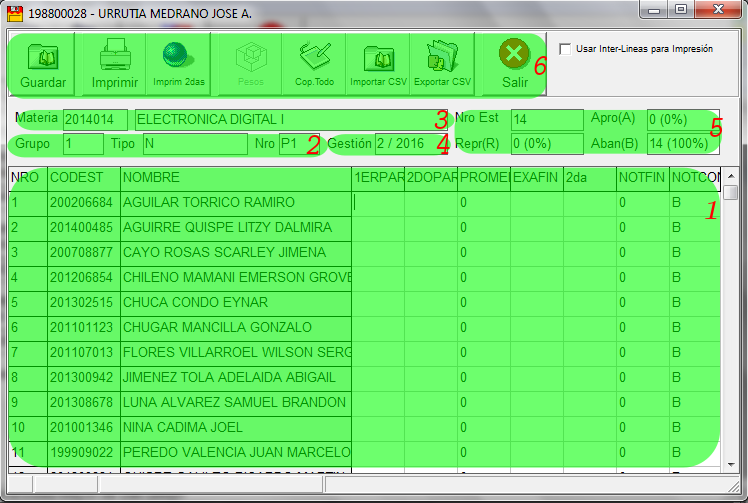
\includegraphics[width=0.6\textwidth]{td3.png}
\captionsetup{justification=centering, margin=2cm}
\caption{Detalle de la lista de estudiantes Fuente: Proporcionado por el MEMI}
\label{fig:Caso2T}
\end{figure}

La lista de estudiantes se divide en las siguientes partes, las cuales est'an enumeradas detalladamente en la siguiente lista:
\begin{enumerate}
\item La lista de estudiantes consta con los siguientes datos: n'umero, c'odigo, nombre, 1er parcial, 2do parcial, promedio, examen final, 2da instancia, nota final y nota contado.
\item Los datos del grupo son: c'odigo de reconocimiento, tipo y n'umero de grupo.
\item Los datos de la materia son: el c'odigo y nombre.
\item El dato de gesti'on.
\item En los datos extra de los estudiantes estan : la cantidad, porcentaje de reprobado, aprobado y abandonado.
\item La lista de men'u son guardar, imprimir, imprimir 2da instancia, pesos, copia todo, importar csv, exportar csv y salir.
\end{enumerate}
\end{enumerate}

\subsection{Las restricciones del transcriptor}
La aplicaci'on del transcriptor, seg'un el detalle y la funcionalidad, tiene las siguientes restricciones:
\begin{enumerate}
\item Se puede usar 'unicamente en el sistema operativo windows.
\item Solo permite abrir archivos con la extensi'on sis.
\item No permite abrir un documento de planilla de notas, si estas da'nado.
\item Controla los datos a ser insertados.
\item Protege la informaci'on del archivo y solo permite modificar la nota del estudiante.
\item Solo permite modificar la planilla de nota por grupo.
\item No permite cerrar la lista de grupos, sin previamente haber guardado.
\end{enumerate}

Despu'es de concluir con el an'alisis del transcriptor, se empieza a analizar el contenido de la planilla de notas que tiene la extensi'on sis.

\section{La planilla de notas}
El documento de la planilla de notas es un  est'andar que utiliza la UMSS\footnote{UMSS-Universidad Mayor de San Sim'on} para la modalidad de calificaci'on de las diferentes carreras. Para explicar la utilidad de la planilla de notas se divide en  la informaci'on y la estructura de la planilla de notas.


% aqui me quede
\subsection{La informaci'on de la planilla de notas}
La informaci'on se divide en datos academicos, la estructura del formato de los grupos, la estructura de los grupos y estructura de la informaci'on del estudiante. En el siguiente p'arrafo se explicara.
\begin{enumerate}
\item  Los datos academicos se explica en cada lin'ea del documento de la planilla de notas, la c'ual tiene la siguiente estructura.
\begin{verbatim}
PCD5.0 //codigo inicio
2719  //codigo fin
09/08/2016 //fecha de creacion
09/08/2016 //fecha de creacion
198800028 //codigo docente
URRUTIA MEDRANO JOSE A.//nombre y apellido docente
299701//codigo carrera
LICENCIATURA EN INGENIERIA ELECTRICA //nombre carrera
2016// gestion
1 //numero gestion
Primer Semestre //literal del semestre
20 //codigo facultad
CIENCIAS Y TECNOLOGIA //nombre facultad
11 //codigo UPSI
UPSI nombre Upsi
263 //tipo de template
tecno //carrera de template
26	//nota maxima para el template
\end{verbatim}
\item La estructura del formato de grupos se explica en forma horizontal del documento de planilla de notas.\\
\begin{verbatim}
\\a,b   ,c ,d,e  ,f,g ,h ,i,j,k   
1,NUMERO,RD,0,100,,NRO,38,N,N,NONE
.........
10,NOTCON,RD,0,100,ARB,NOTCON,50,N,N,ERES
\end{verbatim}
\begin{enumerate}
\item 1 es el orden de la fila.
\item NUMERO es identificador de la  etiqueta ordenado por fila.
\item RD o WR permiso de lectura o escritura.
\item 0 es el inicio del rango de datos.
\item 100 o 51  es el final del rango de datos.
\item A o R o B  es el valor permitido.
\item NRO nombre de la etiqueta ordenado por fila.
\item 38 o 72 o 230 o 52 o 50 ancho de la columna.
\item N para habilitar si tiene nota final.
\item N para habilitar si tiene segunda instancia.
\item NONE palabra reservado.
\end{enumerate}
La estructura del formatos de los grupos depende del formato de calificaci'on es por lo c'ual el grupo normal tiene 10 columnas y el grupo mesa tiene 7 columnas.

\item La estructura del formato de los grupos se divide por la coma se explican a continuaci'on de manera secuencial.\\
Detalle grupo normal:
\begin{verbatim}
\\a, b,   ,c, d 				  ,e  , f ,g,h ,i ,j,k,l,m 	
P1,2014014,1,ELECTRONICA DIGITAL I,263,100,0,50,50,0,0,0,0
P2,2014014,ME,ELECTRONICA DIGITAL I,263,100,0,50,50,0,0,0,0
\end{verbatim}
\begin{enumerate}
\item P1 o P2 es el c'odigo grupo.
\item 2014014 es el c'odigo de la materia.
\item 1 o ME es el tipo de grupo.
\item ELECTRONICA DIGITAL I es el nombre de la materia.
\item 263 es el tipo de template.
\item 100 es el peso global de T1, T2 y T3.
\item 0 es el peso del examen final.
\item 50 es el T1.
\item 50 es el T2.
\item 0 es el T3.
\item 0 es el P1
\item 0 es el P2.
\item 0 es el P3.
\end{enumerate}
Los datos que empieza con la letra P son los parciales y los datos que empieza  con la letra T son los trabajos.
\item La estructura de la informaci'on del estudiante    se divide en grupo normal y mesa como se muestra a continuaci'on.
\begin{enumerate}
\item Lista de estudiantes de grupo normal tiene 10 columnas como se muestra en la siguiente linea del documento:
\begin{verbatim}
1,200206684,AGUILAR TORRICO RAMIRO,,,,,,,
\end{verbatim}
La estructura de la informaci'on del estudiante se explica de manera secuencial los cuales son: 1 es NRO, 200206684 es COD, AGUILAR TORRICO RAMIRO es NOMEST, vacio es 1ERPAR , vacio es 2DOPAR, vacio es PROMED, vacio es EXAFIN, vacio es 2da, vacio es NOTFIN y vacio es NOTCON.
\item Lista de estudiantes del grupo mesa tiene 7 columnas, seg'un la siguiente linea del documento:
\begin{verbatim}
1,201209060,CALIZAYA MAMANI GAITH EFRAIN,20,,20,R
\end{verbatim}
La lista de estudiantes se desarrollan de forma ordenada estas son: 1 es NRO, 200206684 es COD, CALIZAYA MAMANI GAITH EFRAIN es NOMEST, 20 es 1RAOPC, vacio es 2DAOPC, 20 es NOTFIN y vacio es NOTCON.
\end{enumerate}
\end{enumerate}

\subsection{La estructura de la planilla de notas}
La estructura de la planilla de notas tiene una estructura de etiqueta de inicio y final el c'ual divide a la informaci'on en una manera organizada para el reconocimiento del transcriptor.exe. A continuaci'on se explica el orden de la estructura de la planilla de notas.
\begin{verbatim}
<pcd>(inicio documento)
<head>(inicio cabecera)
<info>(inicio Informacion)
</info> (fin Informacion)
<columna> (inicio columna)
<template> (inicio template)
<normal> (inicio normal)
</normal>(fin normal)
<me>(inicio mesa)
</me>(fin mesa)
</template>(fin template)
</column>(fin columna)
<group>(inicio de grupo)
  <normal>(inicio de grupo normal)
  </normal>(fin de grupo normal)
  <me>(inicio de grupo mesa)
  </me>(fin de grupo mesa)
</group>(fin de grupo mesa)
</head>(fin de cabecera)
<body>(inicio cuerpo)
<gradelist>(inicio de lista)
<P1>(inicio materia tipo)
</P1>(fin materia tipo)
<P2>(inicio materia tipo)
</P2>(fin materia tipo)
</gradelist>(fin de lista)
/body>(fin cuerpo)
</pcd>(fin documento)
\end{verbatim}

\subsection{Las restricciones de la planilla de notas}
La planilla de notas es un archivo con extensi'on sis que tiene las siguientes restricci'on:
\begin{enumerate}
\item No se debe cambiar la extensi'on.
\item No se debe alterar la estructura del archivo en caso contrario no sera reconocido por la aplicaci'on del transcriptor.exe.
\end{enumerate}                

En conclusi'on  se puede notar que  la funcionalidad de modificar la planilla de notas tiene 3 procesos en los cuales se utilizan las siguientes aplicaciones: la p'agina del SAGAA\footnote{SAGAA - Sistema de Apoyo a la Gesti'on Acad'emica y Administrativa} y el transcriptor.exe. Tomando en cuenta que cada uno tiene su respectiva restricci'on es por este motivo que se elige esta misma como una herramienta de prueba. 
\chapter{Proceso de desarrollo de servicio}
\label{capitulocuatro}
%El proceso de desarrollo de servicio web representa la abstracci'on de reutilizaci'on de una aplicaci'on a tr'aves del analisis, los detalles del dise'no, la clasificaci'on del tipo de servicio ofrecido y las etapas de la ingenier'ia de servicio.

%Un componente de software de reutilizaci'on, debidamente ajustado, que ofrece  funcionalidad, se  distribuye y se accede de manera
%program'atica. Un servicio Web es un servicio al que se accede mediante protocolo est'andar de Internet y en XML\footnote{Lenguaje de Marcado Extensible}.
%aumentado por mi
%La revoluci'on del software y el desarrollo de la web en la d'ecada de 1990 mejoro el intercambio de informaci'on entre organizaciones. Las computadoras p'odian obtener informaci'on de organizaciones externas. Es por lo c'ual se propuso la noci'on de servicios web con el objetivo  de apoyar en el intercambio de informaci'on entre organizaciones.
El desarrollo de software y la web en los a'nos de 1990 mejoro el intercambio de informaci'on entre las organizaciones. A traves del proceso de desarrollo de servicios web con el fin de apoyar en el intercambio de informaci'on entre las organizaciones.
\section{El servicio web como componente de reutilizaci'on}
Seg'un Somerville " los servicio web son un desarrollo natural de los componentes de software. Una diferencia fundamental entre un servicio y un componente de software, es que el servicio debe ser independiente y opera en la misma forma, sin importar su entorno de ejecuci'on."\hfill \break
Este servicio web define lo que necesita de otro servicio al establecer sus requerimientos en un mensaje y al enviar el mensaje con la especificaci'on y los detalles de su interfaz. Los cuales se explican a continuaci'on en los documentos de lenguaje de descripci'on de servicios web como WSDL\footnote{WSDL-Lenguaje de descripci'on de servicios web} \cite{Somerville2011}. 
\begin{itemize}
\item En el documento de interface se define las operaciones que soportan el servicio y el formato de los mensajes que env'ian y reciben por parte del mismo servicio.
\item En el documento de enlace mapea la interfaz abstracta a tr'aves de un conjunto concreto de protocolos y especifica los detalles t'ecnicos de c'omo comunicarse con el servicio.
\item En el documento de ubicaci'on se describe la ubicaci'on de la implementaci'on del servicio web en su punto final.
\end{itemize}
El desarrollo de WSDL expresa el servicio web en el formato XML.
\section{La ingenier'ia de servicio}
%Esto es parafraseo
La ingenieria de servicio web es el proceso de desarrollo de servicios para la reutilizaci'on en aplicaciones orientadas a servicios. La ingenier'ia de servicio garantiza que el servicio represente la abstracci'on y la reutilizaci'on, los cuales son 'utiles para otros sistemas. \cite{Somerville2011}. 

Seg'un Somerville exiten tres etapas l'ogicas en el proceso de ingenier'ia de servicio, el c'ual se representa a continuaci'on en la figura \ref{DiagramaIngenieria} y la descripci'on de cada etapa. 
\begin{figure}[H]
\centering
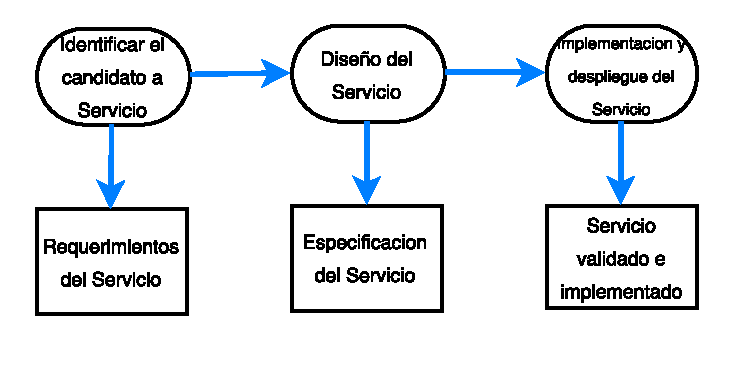
\includegraphics[width=0.6\textwidth]{DiagramaIS.pdf}
\captionsetup{justification=centering,margin=2cm}
\caption{El proceso de ingenier'ia de servicio, adoptado para la realizac'ion del proyecto. El proceso de ingenier'ia de servicio \cite{Somerville2011}}
\label{DiagramaIngenieria}
\end{figure}
La descripci'on de cada etapa l'ogica se explica en las siguientes etapas: 
\begin{itemize}
\item \textbf{Identificaci'on de candidatos a servicios:} la identificaci'on orientada a servicio implica comprender y analizar los procesos empresariales de la organizaci'on para decidir cu'ales servicios de reutilizaci'on podr'ian implementarse. Existen tres tipos de servicios para identificar el servicio los cuales son: servicio utilitario, servicio empresarial y servicio de coordinaci'on o proceso.
El presente proyecto es tipo empresarial porque se trata de servicios asociados con una funci'on empresarial especifica. Para verificar si el servicio es 'util, se plantean las siguientes preguntas las cuales son:\\
\textbf{El cuestionario:} ayuda a reconocer el servicio y verificar el servicio.
\begin{enumerate}
\item ?` El servicio de entidades esta asociado a una entidad l'ogica que se utiliza en diferentes procesos empresariales?
\item ?` Que operaciones soporta la entidad ?
\item ?` Se trata de tareas que realizan diferentes personas en la organizaci'on?
\item ?` El servicio es independiente?
\item ?` El servicio tiene estado?
\item ?` El servicio pueden usar el cliente fuera de la organizaci'on?
\item ?` Diferentes usuarios tienen diferentes requerimientos?
\end{enumerate}
Las respuestas  ayudan a seleccionar y refinar abstracciones para implementar el servicio.
El resultado del proceso de selecci'on de servicios es un conjunto de servicios identificados y requerimientos funcionales del servicio, el cual define que debe hacer el servicio.
\item \textbf{Dise'no de interfaces del servicio:} el dise'no de interface define las operaciones asociadas con el servicio y sus par'ametros. Existen tres etapas en el dise'no de la interfaz del servicio:
\begin{itemize}
\item En el dise'no de interfaz l'ogica comienza con los requerimientos del servicio y define los nombres, par'ametros  de entrada salida, de operaci'on y excepciones.
\item En el dise'no de mensajes se define la estructura de los mensajes que env'ian y reciben el servicio.
\item Desarrollo de WSDL es el dise'no l'ogico y de mensajes se traducen a una descripci'on de interfaz abstracta como se explica anteriormente el documento de interface, el documento de enlace y el documento de ubicaci'on.
\end{itemize}

\item \textbf{Implementaci'on y despliegue del servicio:} una vez concluido los candidatos y los dise'nos de interfaces, la etapa final del proceso de ingenier'ia de servicios es la implementaci'on del servicio. 
\end{itemize}
%aquiiii
\section{Servicios de sistemas heredados}
Seg'un Somerville " los sistemas heredados son sistemas de software antiguos que emplea una organizaci'on, en lo general dependen de tecnolog'ia obsoleta, pero son esenciales para la empresa." Los servicios que se desarrollan para acceder al sistema heredado son coherentes y soportan una sola 'area de su funcionalidad, los cuales se pueden representar graficamente en un diagrama de UML\footnote{UML- Unidad de Lenguaje Modificado}.\cite{Somerville2011}

\section{Desarrollo de software con servicios}
Seg'un Somerville el " desarrollo de software utiliza el  servicio, el c'ual se basan en la idea de que usted combina y configura servicios para crear nuevos servicios compuestos. Estos pueden integrarse con una interfaz de usuario implementada en un navegador para crear una aplicaci'on web".\\
El desarrollo de software con servicios es el proceso de dise'nar nuevos servicios  reutilizando los servicios existente.\\
Seg'un Somerville en la siguiente figura se muestra las etapas de construcci'on de servicio mediante composici'on: 

\begin{figure}[H]
\centering
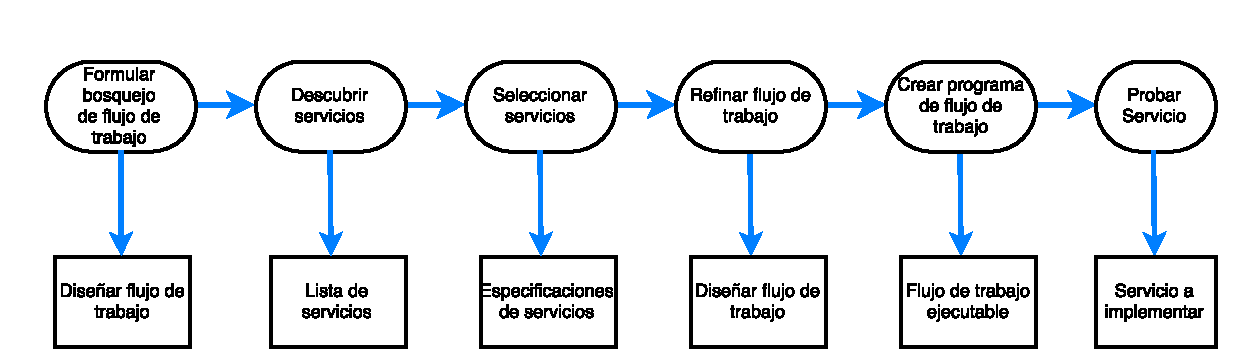
\includegraphics[width=0.8\textwidth]{construirServicio.pdf}
\captionsetup{justification=centering,margin=2cm}
\caption{Etapas de la Construcci'on de servicio, adoptado para la realizac'ion del proyecto. Construci'on de servicio\cite{Somerville2011}}
\label{fig:construccion}
\end{figure}

\begin{itemize}
\item \textit{Formular un bosquejo de flujo de trabajo} comienza con los requerimientos para crear un servicio compuesto, el c'ual es la base para un nuevo dise'no.
\item \textit{El descubrimiento del servicio} se buscan los registros o catalogos de los servicios para descubrir cuales servicio existen, qui'en los proporciona y los detalles de la provisi'on del servicio.
\item \textit{Seleccionar posibles servicios} a partir del conjunto de posibles candidatos a servicio que se han descubierto se seleccionan los posibles servicios que puedan implementar actividades del flujo de trabajo.
\item \textit{Refinar el flujo de trabajo} sobre la base de la informaci'on acerca de los servicios que se selecciona y  se refine el flujo de trabajo.
\item \textit{Crear un programa de flujo de trabajo} durante la etapa el dise'no de flujo de trabajo abstracto se transforma en un programa ejecutable.
\item \textit{Prueba de servicio o aplicaci'on terminada} es el proceso de probar el servicio terminado para realizar la prueba se utilizan los servicios externos.
\end{itemize}
Para concluir se explica el dise'no y las pruebas del flujo de trabajo. Uno de los problemas es la  reutilizaci'on dentro de la organizaci'on.


\subsection{Dise'no e implementaci'on del flujo de trabajo} 
Seg'un Somerville " dise'no de flujo de trabajo implica analizar los procesos empresariales existentes o planeados para comprender las diferentes actividades que se realizan, estas intercambian informaci'on, luego se define el nuevo proceso empresarial en la notaci'on de flujo de trabajo".  
Si los procesos empresariales tienen  diferentes partes de una organizaci'on estas se pueden separar mediante carriles. 
Una vez concluido con el dise'no final, el c'ual se debe convertirse en un programa ejecutable. \cite{Somerville2011}
\begin{itemize}
\item \textit{Implementar los servicios} se debe tener en cuenta que los servicios son independientes del lenguaje de implementaci'on.
\item \textit{Generar una versi'on ejecutable} del modelo de flujo de trabajo traducirlo a un c'odigo de manera manual o automatica.
\end{itemize}
\subsection{Pruebas del servicio} 
Las pruebas son importantes para los procesos de desarrollo de sistemas, estos muestran que un sistema cumple con los requerimientos funcionales y detectan defectos introducidos durante el proceso de desarrollo.\cite{Somerville2011} 

Seg'un Somerville " para comprender la implementaci'on del servicio se debe presentar dificultades cuando se prueba el servicio y la combinaci'on de los servicios". 

Seg'un Somerville a continuaci'on los tipos de prueba del servicio.
\begin{enumerate}
\item \textit{Prueba de servicio o aplicaci'on terminada} es el proceso de probar el servicio terminado, es complejo cuando se usa servicios externos.
\item \textit{Los servicios externos} est'an bajo el control de proveedor de servicio y no del usuario del servicio. El proveedor puede retirar los servicios, dicho problema se debe manejar como componentes para mantener las versiones.
\item \textit{Los servicios a largo plazo} la aplicaci'on puede usar otro servicio.
\item \textit{El comportamiento no funcional} no depende solo de como se usa, por parte de la aplicaci'on que se pone a prueba.
\item \textit{El modelo de pago} para los servicios se puede hacer que los servicios sean muy costosos. Se debe utilizar servicios que son gratuitos. 
\end{enumerate}
%debemos unir estas dos figuras que cumpla con la estructura q he definido
%Para el proceso de construcci'on  de servicio mediante composici'on, se muestran 6 etapas en la figura  \ref{fig:construccion}:

%\begin{figure}[H]
%\centering
%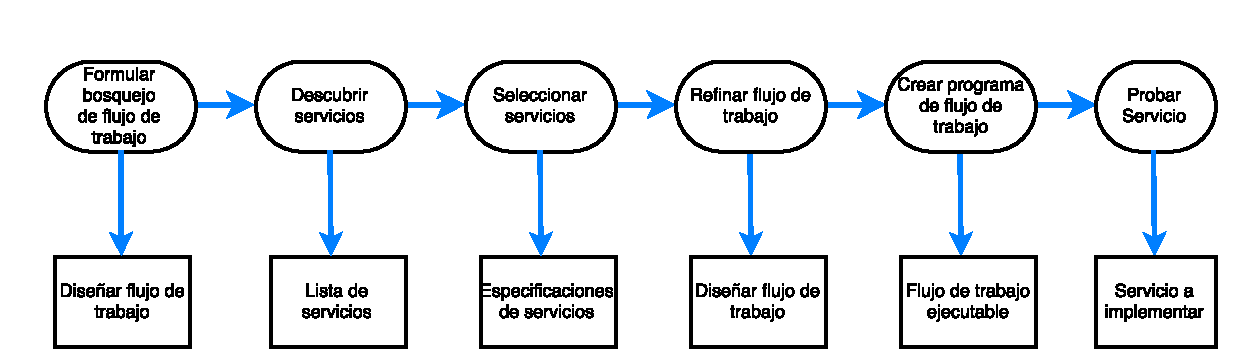
\includegraphics[width=0.8\textwidth]{construirServicio.pdf}
%\captionsetup{justification=centering,margin=2cm}
%\caption{Etapas de la Construcci'on de servicio, adoptado para la realizac'ion del proyecto. Construci'on de servicio\cite{Sommerville2012}}
%\label{fig:construccion}
%\end{figure}
%A continuaci'on se explica cada etapa de la figura  \ref{DiagramaIngenieria} de la ingenier'ia de servicio.


%\section{Tipos de servicio web}
%Se tiene 3 tipos de servicios son: utilitarios, empresariales y coordinaci'on o proceso.Para el presente proyecto, se ha definido un servicio empresarial, que se explica a continuaci'on.

%\begin{itemize}
%\item \textbf{Servicio empresarial,} se trata de servicios asociados, con una funci'on empresarial especifica. Un ejemplo de una funci'on empresarial es una universidad ser'ia la inscripci'on de estudiantes para un curso u otros. 
%\end{itemize}


%\section{Identificar los candidatos a servicio}
%Para identificar el candidato a servicio se debe comprender y analizar los procesos empresariales de la organizaci'on. Los procesos empresariales aportan en la identificaci'on del servicio y desde los procesos se determinan el servicio a ser reutilizado. Este servicio debe ser l'ogicamente coherente, independiente y reutilizado por lo c'ual puede ser orientados a entidades o tareas y estas son asociadas con alguna actividad.
%Para verificar  el candidato al servicio se debe plantear el cuestionario, el proceso de selecci'on y el flujo de trabajo. A continucaci'on se explican el cuestionario, el proceso de selecci'on y el flujo de trabajo.

%\begin{itemize}
%\item \textbf{El cuestionario:} ayuda a reconocer el servicio y verificar si el servicio es 'util. A continuaci'on las preguntas del cuestionario.
%\begin{enumerate}
%\item �El servicio de entidades esta asociado a una entidad l'ogica que se utiliza en diferentes procesos empresariales?
%\item �Que operaciones soporta la entidad ?
%\item �Se trata de tareas que realizan diferentes personas en la organizaci'on?
%\item �El servicio es independiente?
%\item �El servicio tiene estado?
%\item �El servicio pueden usar el cliente fuera de la organizaci'on?
%\item �Diferentes usuarios tienen diferentes requerimientos?
%\end{enumerate}
%Despues de terminar el cuestionario se analiza las respuestas, para comenzar analizar el proceso de selecci'on.
%\item \textbf{Proceso de selecci'on:} es un conjunto de actividades orientadas para realizar parte del trabajo con el fin de alcanzar una meta de los servicios identificados, el c'ual  tiene 6 etapas claves de proceso de construcci'on las cuales se explican a continuaci'on:

%\begin{enumerate}
%\item Formular el bosquejo de flujo de trabajo se usan los requerimientos para el servicio compuesto con el fin de conocer los servicios disponibles.
%\item Descubrimiento de servicios se buscan los servicios existente, qui'en los  proporciona y los detalles.
%\item Seleccionar posibles servicios a partir de los candidatos a servicios y teniendo en cuenta los criterios de selecci'on incluir'an  las funcionalidades de los servicios ofrecidos.
%\item Refinar el flujo de trabajo sobre la base de la informaci'on acerca de servicio que se han seleccionado se refina el flujo de trabajo. Se vuelve a repetir la etapa de descubrimiento y selecci'on. 
%\end{enumerate}

%inicio de aumentado
%\item \textbf {Dise'no de Flujo de trabajo}
%Es el conjunto de actividades orientadas para realizar parte del trabajo, el c'ual establece los pasos necesarios para alcanzar Los detalles del flujo de trabajo ayudan a organizar las actividades del servicio web las cuales son:
%\begin{enumerate}
%\item \textbf{Flujo de trabajo,} es un conjunto de actividades orientadas para realizar parte del trabajo, el c'ual establece los pasos necesarios para alcanzar una meta particular.
%El dise'no de flujo de trabajo analiza los procesos planeados, al comprender las actividades, al realizar el intercambio de informaci'on, para definir las etapas de proceso.
%El flujo de trabajo se representa en el diagrama de actividades de UML\footnote{Unidad de Lenguaje Modificado}.
%Tiene algunos conceptos centrales de BPMN\footnote{Proceso de Negocio de Modelo de Notaci'on}, se utiliza para crear el modelo de flujo de trabajo.  A continuaci'on se explica los detalles del flujo de trabajo.
%\begin{itemize}
%\item La actividad se representan mediante un rect'angulo con esquinas redondeadas. Una actividad puede ejecutarse por una persona o por un servicio automatizado.
%\item El evento se representa en c'irculo. Un evento es algo que sucede durante un proceso: evento inicial(c'irculo claro), evento final(c'irculo oscuro), evento intermedio (c'irculo doble no se muestra) se ejecuta peri'odicamente.
%\item Las compuertas se representa mediante un diamante, es una etapa en el proceso para utilizar una elecci'on.
%\item La secuencia de actividades, se representa mediante una flecha s'olida, se usa para mostrar la secuencia de actividades. El mensaje que fluyen entre actividades se representan en una flecha punteada.
%\end{enumerate}
%\end{itemize}
%\item \textbf{Acci'on de compensaci'on}
%La acci'on de compensaci'on se utiliza para deshacer acciones, que se completan, el c'ual deben cambiar el resultado de posteriores actividades del flujo de trabajo.
%\end{enumerate}


%fin de aumentado

%\section{El dise'no de servicio web}
%Una vez concluida, con  la identificaci'on del servicio, se realiza las operaciones asociadas con el servicio y sus p'arametros, el dise'no de operaciones y los mensajes de servicio. El dise'no se representa en 3 tipos, para el presente proyecto se utiliza los siguientes: 
%\begin{enumerate}
%\item Dise'no de interfaz l'ogica, se identifica las operaciones asociadas con el servicio, sus entradas y salidas, as'i como las excepciones asociadas con dichas operaciones. Despu'es se realiza los requerimientos del servicio, define los nombres y par'ametros de operaci'on. Se debe definir las excepciones que s'urgen cuando se ubica una operaci'on de servicio.
%\item Dise'no de mensajes, es la estructura de los mensajes que env'ia y recibe el servicio. Define los mensajes de entrada y salida, el manejo de mensajes como objetos, la estructura en operaci'on y excepciones.
%\end{enumerate}

%Una vez concluido, con el dise'no para an'alisis del servicio, se realiza el dise'no para desarrollar el servicio con flujo de trabajo.

%\begin{enumerate}
%\item \textbf{Crear un programa de flujo de trabajo,} es  el dise'no de flujo de trabajo, para transformar en un programa ejecutable.
%\item \textbf{Crear un dise'no de datos de servicio,} es el dise'no para mostrar el formato de informaci'on, para utilizar el servicio web. 
%\end{enumerate}


%\section{Implementaci'on del servicio web}

%El modelo puede realizar algunas iteraciones, hasta que se cree un dise'no que permite la reutilizaci'on de los servicios disponibles.
%Utilizamos el dise'no de desarrollo del servicio de flujo de trabajo, que se debe convertira en un programa ejecutable, esto implica la actividad de:
%\begin{enumerate}
%\item Implementar los servicios, los servicios son independientes del lenguaje de implementaci'on, dichos servicios se pueden escribir en cualquier lenguaje de programaci'on.
%\end{enumerate}

%\section{Pruebas del servicio}
%Las pruebas son importante en todos los procesos de desarrollo del sistema se muestran que un sistema cumple con los requerimientos funcionales cuando se utiliza un servicio externo 'esto significa que no se tiene acceso a su co'digo fuente es por lo c'ual que no se debe hacer en base a c'odigo fuente.
%Para comprender lo implementaci'on se debe realizar prueba y combinaci'on de los servicios:
%\begin{itemize}
%\item \textbf{Prueba de servicio o aplicaci'on terminada,} es el proceso de probar el servicio terminado, es complejo cuando se usa servicios externos.
%\item \textbf{Los servicios externos,} est'an bajo el control de proveedor de servicio y no del usuario del servicio. El proveedor puede retirar los servicios, dicho problema se debe manejar como componentes para mantener las versiones.
%\item \textbf{Los servicios a largo plazo,} la aplicaci'on puede usar otro servicio.
%\item \textbf{El comportamiento no funcional,} no depende solo de como se usa, por parte de la aplicaci'on que se pone a prueba.
%\item \textbf{El modelo de pago,} para los servicios se puede hacer que los servicios sean muy costosos. Se debe utilizar servicios que son gratuitos. 
%\end{itemize}

\section{El dise'no metodolog'ico}
El dise'no metodolog'ico para el presente proyecto se realizo en base a la puntos anteriores teniendo como resultado la siguiente figura \ref{fig:Diagrama} que representa la secuencia de procesos de desarrollo para este proyecto.

\begin{figure}[H]
\centering
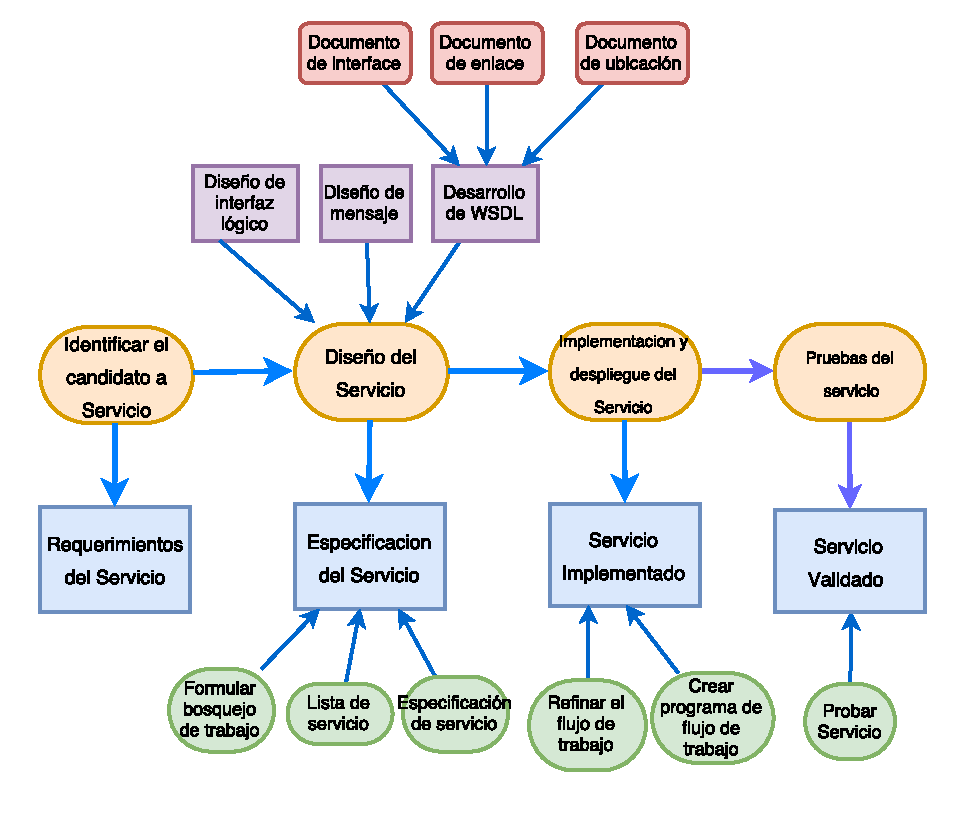
\includegraphics[width=0.7\textwidth]{DiagramaDServicio.pdf}
\captionsetup{justification=centering, margin=2cm}
\caption{Secuencia de pasos para el proceso de ingeniera. Fuente: En base a la construcci'on de servicio de Somerville \cite{Somerville2011}}
\label{fig:Diagrama}
\end{figure}

El presente proyecto es un sistemas heredado porque utiliza como antecedente a la p'agina del SAGAA para el desarrollo del servicio web. Es por lo c'ual se ha incorporado las etapas de construcci'on de servicio mediante composici'on  en el modelo metodol'ogico.

\section{Conclusiones}
La arquitectura de servicios web utiliza el desarrollo de componentes como base para la etapa de construcci'on del servicio web.

Los sistemas heredados utilizan un servicio web existente de una organizaci'on para crear un nuevo servicio web con la herramienta de diagrama de flujos de trabajo.

El dise'no metodol'ogico utiliza el dise'no de servicio como base y complementa con la herramienta del desarrollo de software de servicio por componentes para la etapa de dise'no del servicio con los diagrama de flujos.

%En el cap'itulo \ref{capitulocuatro} se explicar'a el proceso de ingenier'ia de software del SOA y en el c'apitulo \ref{capitulodos}, se explican las herramientas para cumplir con el objetivos de \textit{Proveer servicio web de la p'agina del SAGAAA} \ref{sec:oe} en el presente proyecto.\\

%En el cap'itulo \ref{capitulotres} se explica los detalles y procesos para cumplir con el objetivo 1 y la recolecci'on de datos.\\

%En el c'apitulo \ref{capitulocinco} se explica el  analisis, dise'no e implementaci'on del servicio web, como se muestra en la figura \ref{fig:Diagrama} en el n'umero 1 - 3 para cumplir con el objetivo 4.\\
 
%En el c'apitulo \ref{capituloseis}, se explica el analisis y dise'no de la aplicaci'on m'ovil, como se muestra en la figura \ref{fig:Diagrama} en el n'umero 4, para cumplir con el objetivo 4 y en parte al objetivo 1 del c'ual se tiene a continuaci'on el c'apitulo \ref{capitulosiete}, en donde se realiza la implementaci'on de la aplicaci'on m'ovil, como se muestra en la figura \ref{fig:Diagrama} en el n'umero 5 cumpliendo con el objetivo 1 y 3.\\
%En el c'apitulo \ref{capitulonueve} se trata de la prueba de la aplicac'ion m'ovil y el servicio web, como se muestra en la figura \ref{fig:Diagrama} en el n'umero 6, para cumplir con el objetivo general \ref{og} de proveer el servicio del SAGAA, a tr'aves de una aplicaci'on m'ovil.\\

%En el c'apitulo \ref{capituloocho} es el dise'no adaptativo de la aplicaci'on m'ovil que responde al objetivo 2.

%Para el desarrollo de la metodologia se utiliza las siguentes plataformas de desarrollo, se explican a continuaci'on.
\chapter{Dise'no e implementaci'on del servicio web}
\label{capitulocinco}
El desarrollo del servicio en el presente proyecto es para crear un nuevo servicio que garantiza la abstracci'on y la reutilizaci'on de la p'agina del SAGAA.

%El desarrollo del servicio web proporciona el analisis de las actividades y la comunicaci'on de la p'agina del SAGAA, a tr'aves de los dise'nos para ofrecer una explicaci'on logicamente coherencia e independiente.


\section{Identificar el candidato a servicio}
Para identificar el candidato a servicio sin embargo la experiencia y la habilidad en el desarrollo de servicios web.\\
El presente proyecto tiene el objetivo de optimizar los procesos de llenar la planilla de notas en la p'agina del SAGAA como se ha mencionado anteriormente en el capitulo \ref{capitulotres}.
%Para el presente proyecto, analizar cada proceso de la p'agina del SAGAA, es identificar la ubicaci'on y descripci'on del detalle de la interfaz. Para el documento de interfaz se utilizan las operaciones que soportan el servicio web y el documento de enlace, se muestra una interfaz abstracta con un conjunto de protocolos.
Para verificar si el servicio es 'util se realiza el cuestionario, el c'ual se desarrolla en el anexo \ref{cuestionario}.
Despues de lo mencionado anteriormente se realiza la lista de requerimientos para el servicio web estos se mencionan a continuaci'on.

\subsection{Requerimientos del servicio web}
\label{requerimientoServicio}
Los requerimientos que se muestran a continuaci'on son un conjunto de servicios los cuales se obtienen a partir de los procesos de llenar la planilla de notas como se ha explicado anteriormente en el capitulo \ref{capitulotres}. 
\begin{enumerate}
%\item Realizar la sesi'on del usuario.
%\item Obtener los datos de la gesti'on de la planilla de nota.
%\item Seleccionar la gesti'on de la planilla de nota.
\item Descargar la planilla de notas seg'un la gesti'on y la carrera corespondiente.
\item Obtener datos de la p'agina del SAGAA para la unidad de datos para compartir la informaci'on de la planilla de notas.
\item Adjuntar la planilla de nota modificada en la p'agina del SAGAA.
\end{enumerate}
Una vez concluido con los requerimientos se avanza a la etapa de dise'no del servicio web.

\section{Dise'no del servicio}
El dise'no del servicio describe la informaci'on al env'iar los mensajes de entrada y salida  de la p'agina del SAGAA al realizar el proceso de llenar la planilla de notas. Las etapas del dise'no de servicio son la: interfaz l'ogica, mensajes, el desarrollo de WSDL y la especificaci'on del servicio. A continuaci'on se explican cada etapa.


\subsection{La etapa de dise'no de interfaz l'ogica}
El dise'no de interfaz l'ogica es la comunicaci'on entre el cliente y el servidor. El servidor almacena informaci'on de la p'agina del SAGAA. Para explicar los procesos para llenar la planilla de notas.

\begin{itemize}
\item \textit{El Dise'no de interfaz l'ogica del proceso de descargar la planilla de notas} se representa en la siguiente figura \ref{fig:DisenoDescargar2} el cual es la secuencia de peticiones ordenadas, los par'ametros de entrada y salida o mensajes y  las direcciones de url.
% Para realizar las peticiones de descarga de la planilla de notas y obtener los datos para realizar el siguiente proceso.
\begin{figure}[H]
\centering
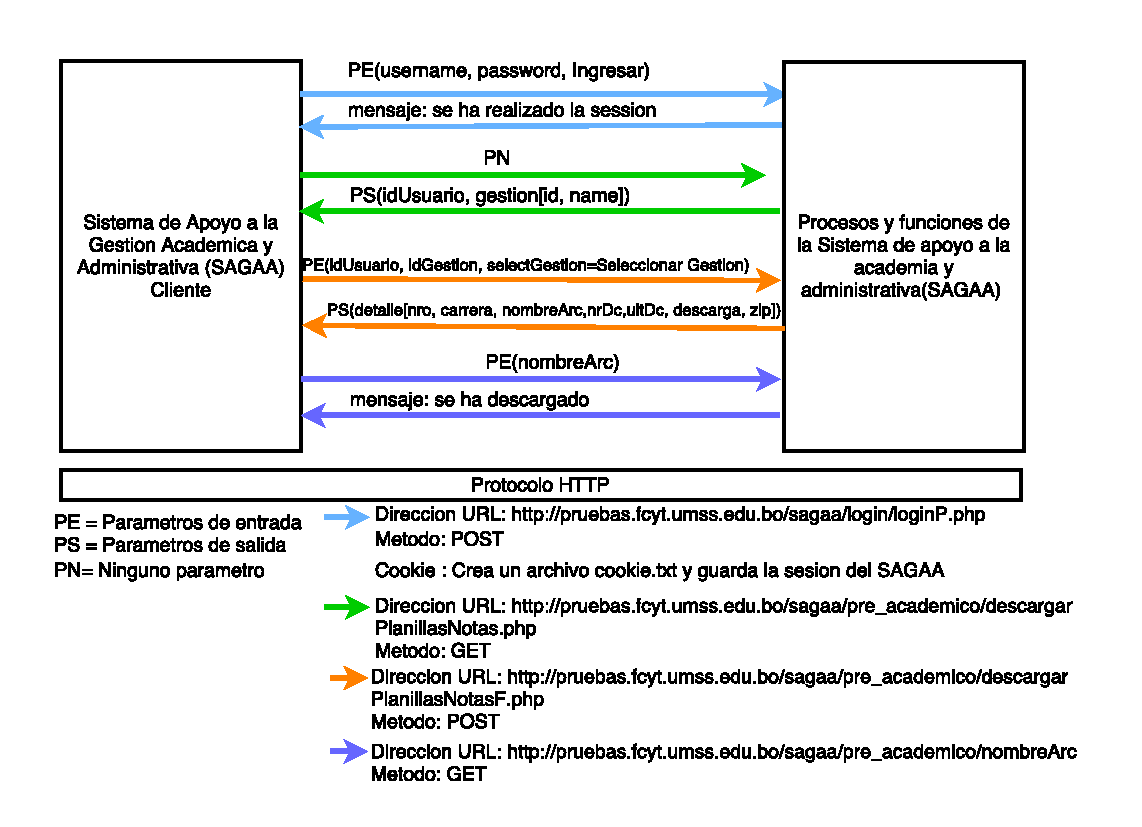
\includegraphics[width=0.7\textwidth]{disenoOperacionDescarga.pdf}
\captionsetup{justification=centering, margin=2cm}
\caption{Dise'no de interfaz l'ogico para descargar la planilla de nota, Fuente: Elaboraci'on propia}
\label{fig:DisenoDescargar2}
\end{figure}

\item \textbf{Dise'no de interfaz l'ogica de adjuntar la planilla de notas,} describe la secuencia de peticiones ordenadas y los parametros de entrada y salida o mensajes y las direcciones de url. Como se muestra en la figura \ref{fig:DisenoSubir}.
% a continuaci'on se expone la secuencia de peticiones ordenas y los parametros de entrada y salida o mensajes y las direcciones de url para realizar el proceso de subir la planilla de notas a la p'agina del SAGAA.
\begin{figure}[H]
\centering
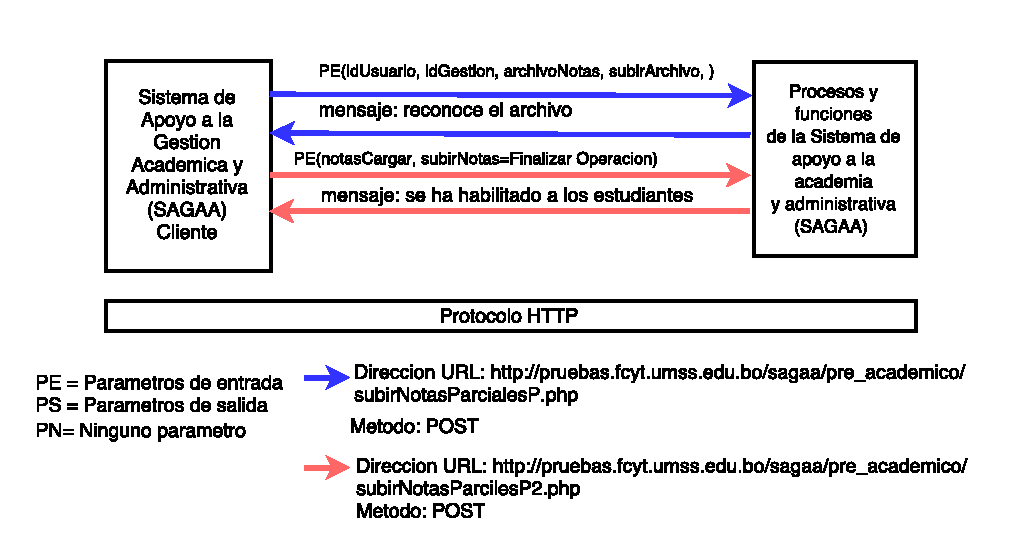
\includegraphics[width=0.6\textwidth]{disenoOperacionSubir.pdf}
\captionsetup{justification=centering, margin=2cm}
\caption{Dise'no de interfaz l'ogico para adjuntar la planilla de notas, Fuente: Elaboraci'on propia}
\label{fig:DisenoSubir}
\end{figure}
\end{itemize}

\subsection{Dise'no de mensaje}
El dise'no de mensaje define la estructura de los mensajes que transcurren en la  comunicaci'on del cliente y servidor cuando se realiza una petici'on.Los mensajes ayudan a mostrar los estados  de la petici'on si es correcta, incorrecta y excepciones. En la siguiente figura \ref{fig:DisenoMensaje} se muestra los mensajes del proceso de llenar la planilla de notas.

\begin{figure}[H]
\centering
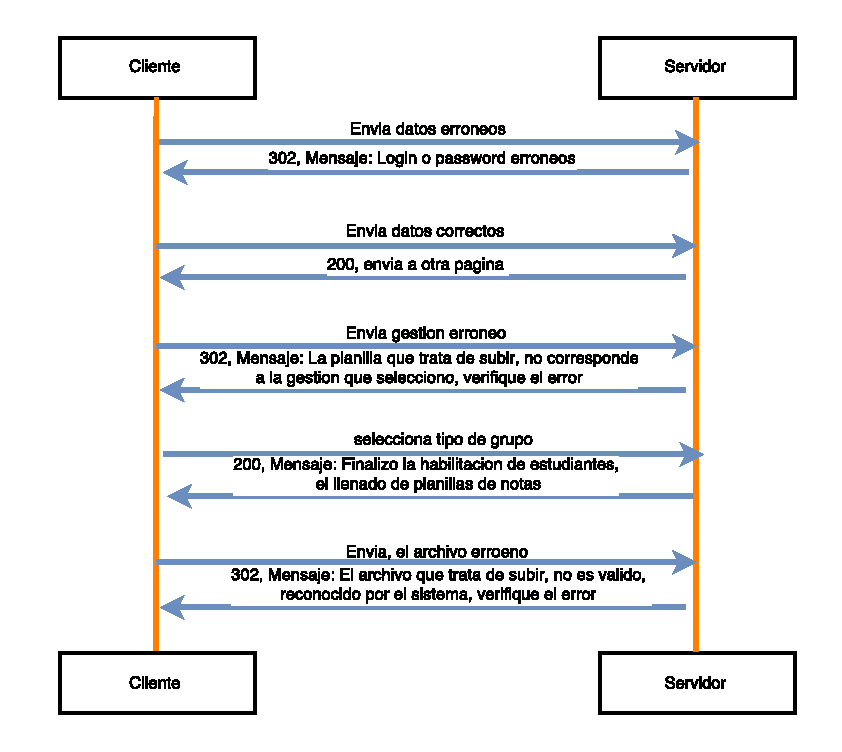
\includegraphics[width=0.6\textwidth]{disenoMensaje.pdf}
\captionsetup{justification=centering, margin=2cm}
\caption{Dise'no de mensaje de entradas, salidas y excepciones, Fuente: Elaboraci'on propia}
\label{fig:DisenoMensaje}
\end{figure}

\subsection{Desarrollo de WSDL}
El desarrollo de WSDL no ha utilizadola estestructura de desarrollo XML  porque utiliza el protocolo REST para la implementaci'on del servicio. El desarrollo de WSDL describe de la interfaz abstracta para llenar la planilla de notas como se explican a continuaci'on en el documento de interface y el documento de enlace.
\begin{itemize}
\item \textbf{Documento de interface}\\
El documento de interface define las operaciones del proceso de llenar la planilla de notas lo cual se dividen en tres procesos los cuales son:
\begin{enumerate}[\bfseries Pr{o}ceso 1:]
 \item Secuencia de procesos para  descargar la planilla de notas en el formato .sis de la p'agina del SAGAA. En la figura \ref{fig:Proceso1}.
 
 \begin{figure}[H]
 \centering
 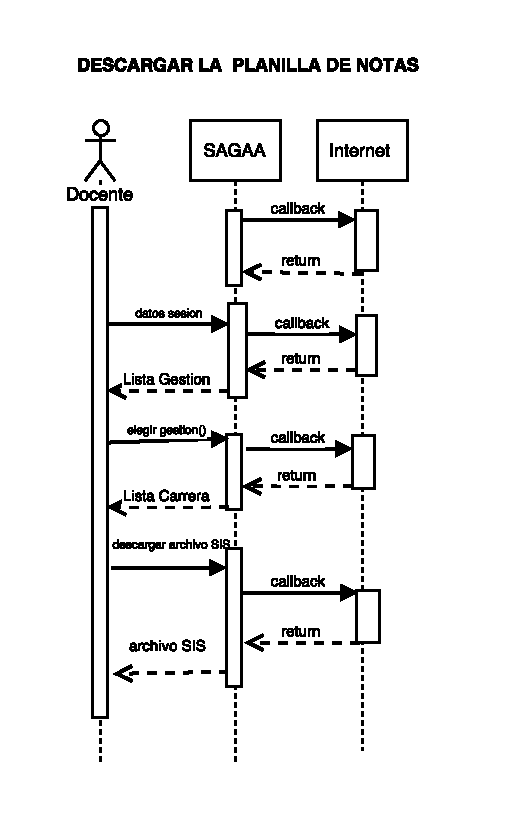
\includegraphics[width=0.3\textwidth]{SdescargarLlenadoNota.pdf}
 \captionsetup{justification=centering,margin=2cm}
 \caption{Proceso de descargar Planilla Notas. Figura: Elaboraci'on propia}
 \label{fig:Proceso1}
 \end{figure}
 
 \item En este proceso se muestran los pasos para modificar la planilla de notas y se ha utilizado la aplicaci'on del Transcriptor.exe para modificar la planilla de notas como se observa en la siguiente figura \ref{fig:Proceso2}.
 
 \begin{figure}[H]
 \centering
 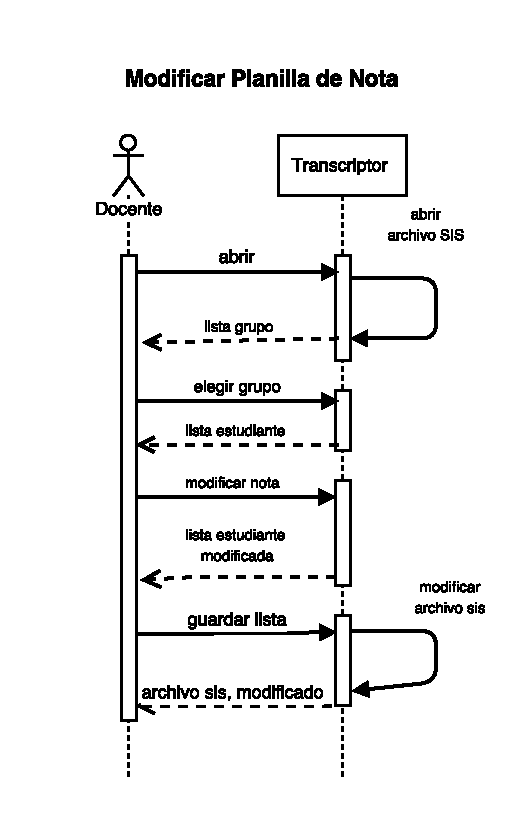
\includegraphics[width=0.3\textwidth]{DSmodificarPlanila.pdf}
 \captionsetup{justification=centering,margin=2cm}
 \caption{Proceso de modificar la Planilla de Notas, Fuente: Elaboraci'on propia}
 \label{fig:Proceso2}
 \end{figure}
   
  \item La ultima secuencia de pasos para adjuntar el archivo de planilla de notas en la p'agina del SAGAA se muestra en la figura \ref{fig:Proceso3}.
  
\begin{figure}[H]
\centering
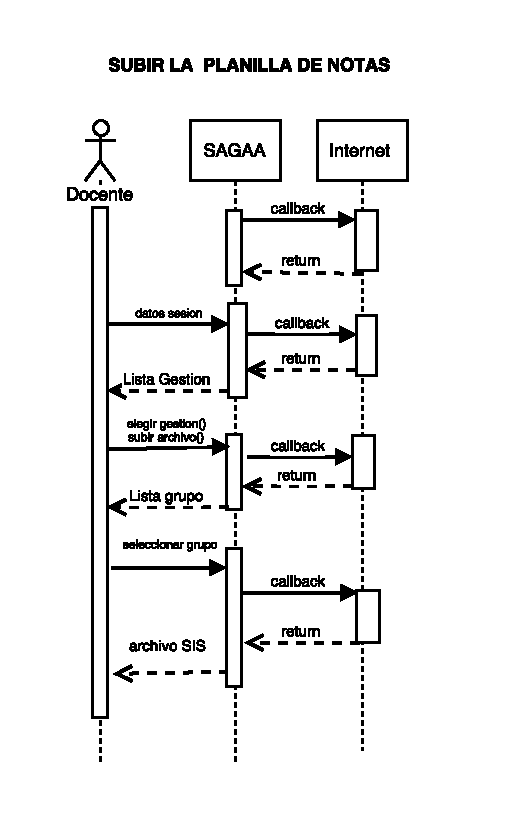
\includegraphics[width=0.3\textwidth]{DSsubirPlanilla.pdf}
\captionsetup{justification=centering, margin=2cm}
\caption{Proceso de subir a la p'agina del SAGAA, Fuente: Elaboraci'on propia}
 \label{fig:Proceso3}
 \end{figure}
\end{enumerate}

\item \textbf{Documento enlace}\\
El documento de enlace es la interfaz abstracta de un conjunto concreto de protocolos los cuales especifican los detalles t'ecnicos de la comunicaci'on entre la p'agina del SAGAA y el servidor. El servidor es donde se almacena la informaci'on solicitada. La interfaz abstracta se representa en la siguiente figura \ref{fig:Comunicacion}.
\begin{figure}[H]
\centering
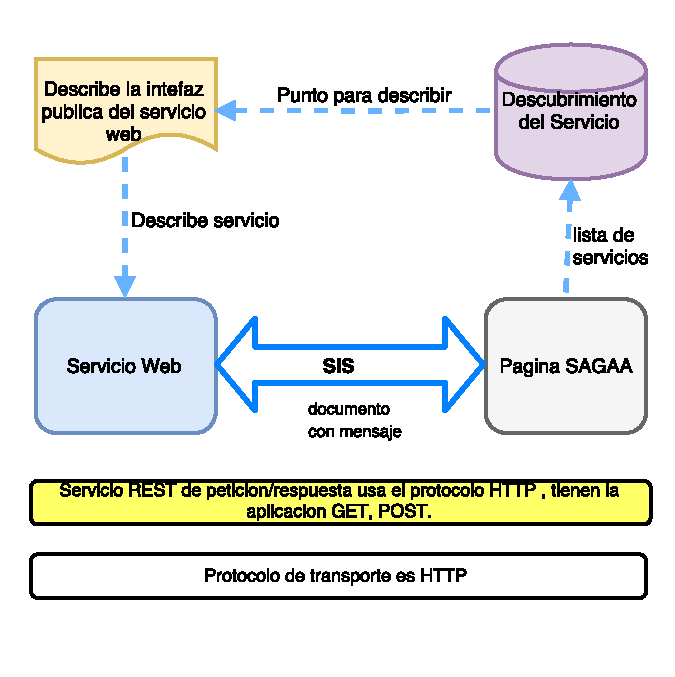
\includegraphics[width=0.4\textwidth]{comunicacioProtocolo.pdf}
\captionsetup{justification=centering, margin=2cm}
\caption{Protocolos de servicio, Fuente: Elaboraci'on propia}
\label{fig:Comunicacion}
\end{figure}

%En la figura \ref{fig:Comunicacion}, se muestran los protocolos que utilizan la p'agina del SAGAA para realizar el proceso de llenar la planilla de notas.

\end{itemize}

\subsection{Especificaci'on del servicio}
En la etapa de especificaci'on del servicio describe las construcci'on de servicios las cuales son: formular el bosquejo de trabajo, lista de servicio y especificaci'on de servicio.
\begin{itemize}
\item \textbf{Formular el bosquejo de flujo de trabajo}\\
A partir de los requerimientos se ha desarrollado un servicio compuesto el c'ual es la base para el nuevo diagrama de flujo de trabajo. Este servicio compuesto describe la secuencia de pasos de llenar la planilla de notas como se observa en la siguiente figura \ref{fig:flujoTrabajo1}.

\begin{figure}[H]
\centering
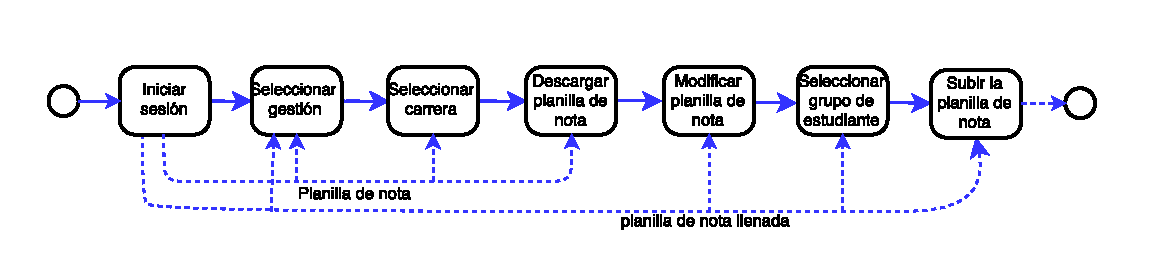
\includegraphics[width=0.9\textwidth]{flujoTrabajo1.pdf}
\captionsetup{justification=centering, margin=2cm}
\caption{Diagrama de flujo de trabajo, Fuente: Elaboraci'on propia}
\label{fig:flujoTrabajo1}
\end{figure}

\item \textbf{Descubrir el servicio}\\
\label{Lista}
Durante la etapa de descubrir el servicio se ha buscado el catalogo o registros para realizar el proceso de llenar la planilla de notas en la p'agina del SAGAA el c'ual se ha obtenido a partir del capitulo \ref{capitulotres}. A continuaci'on la siguiente lista de servicio son:\\

\textbf{Lista de servicio}
\begin{enumerate}
\item Realizar la sesi'on.
\item Listar la gesti'on.
\item Seleccionar la gesti'on
\item Listar las carreras.
\item Seleccionar carrera, para descargar la planilla de notas.
%\item Crear una unidad de datos de la planilla de notas.
\item Subir la planilla de nota modificado.
\end{enumerate}

\item \textbf{Seleccionar el servicio}\\
\label{Especificaciones}
A partir de la lista de servicios se han seleccionado los  candidatos a servicios. Los cuales son los siguientes indices.\\

\begin{enumerate}
\item Para descargar la planilla de notas se realizan la sesi'on del docente,  seleccionar la gesti'on, seleccionar la carrera y por ultimo se descarga la planilla de nota.
\item Modificar la planilla de notas se ralizo a trav'es de la aplicaci'on m'ovil reconocer la planilla de notas, mostrar, modificar y enviar la planilla de notas modificada a la p'agina del SAGAA.
%Modificar la planilla de notas es donde se guarda la planilla de datos localmente, reconoce la planilla de notas, y con la ayuda de la aplicaci'on m'ovil mostrar y modificar la planilla de notas y enviar la planilla de notas modificada a la p'agina del SAGAA.
\item Para subir la planilla de notas primeramente se elige el grupo de materia, luego se adjunta la planilla y por ultimo se selecciona el tipo de grupo para publicar la planilla de notas en la p'agina del SAGAA.
\end{enumerate}
\end{itemize}
%hasta aqui	
\subsection{Implementaci'on y despliegue del servicio}
Al concluir con los dise'nos de interface abstracta se  realizan las etapas de refinar el flujo de trabajo y crear el programa de flujo de trabajo.
\begin{itemize}

\item \textbf{Refinar el flujo de trabajo}\\
A partir de  seleccionar el servicio se realiza el dise'no del servicio. Cada diagrama mejora el detalle y la descripci'on abstracta de cada servicio seleccionado. Cada diagramas mejoran el detalle y la discripci'on abstracta de cada especificaci'on del servicio seleccionado. A continuaci'on se explican cada diagrama de flujo de trabajo.
\begin{itemize}
\item \textit{Descarga la planilla de notas} es la secuencia de procesos para descargar la planilla de notas el c'ual se representa a trav'es del diagrama de flujos de trabajo como se muestra en la siguiente figura \ref{fig:FlujoTrabajoDescargar}.
\begin{figure}[H]
\centering
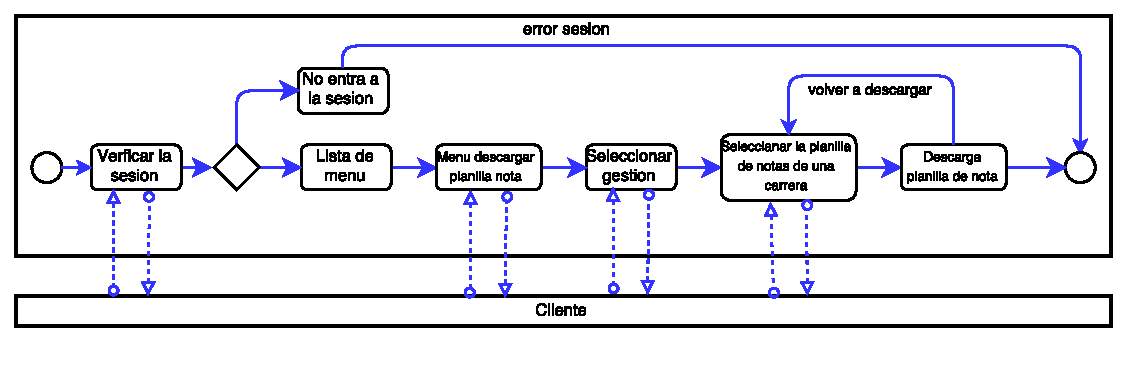
\includegraphics[width=0.8\textwidth]{flujoTrabajoDescarga.pdf}
\captionsetup{justification=centering, margin=2cm}
\caption{Dise'no de flujo de trabajo de descarga de la planilla de notas, Fuente: Elaboraci'on propia}
\label{fig:FlujoTrabajoDescargar}
\end{figure}

\item \textit{Dise'no de modificar la planilla de notas} utiliza la aplicaci'on del Transcriptor.exe el c'ual tiene una secuencia de procesos. En la siguiente figura \ref{fig:FlujoTrabajoModificar} el diagrama de flujo de trabajo. .
\begin{figure}[H]
\centering
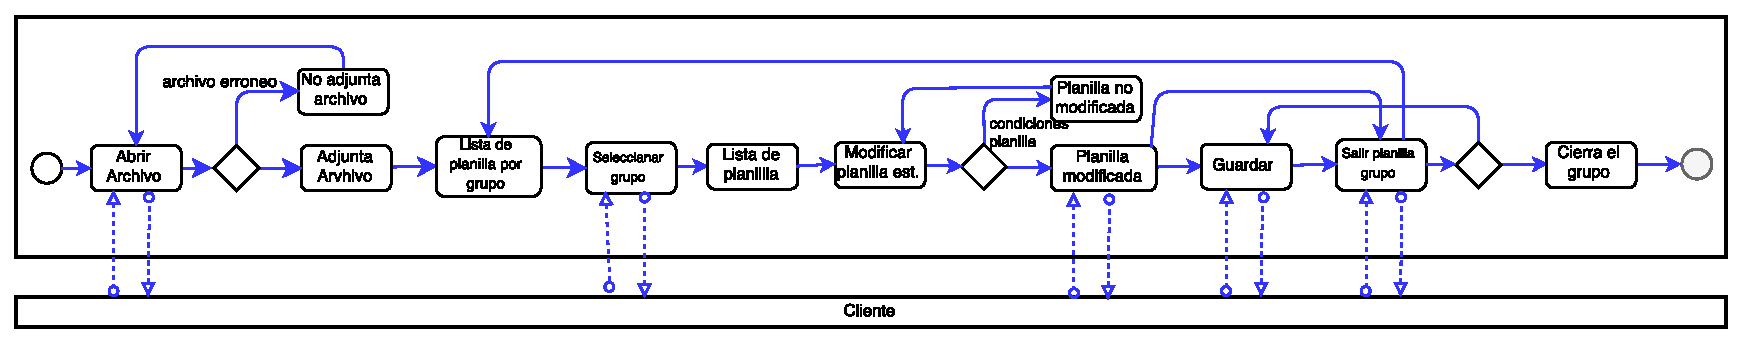
\includegraphics[width=0.8\textwidth]{flujoTrabajoModificar.pdf}
\captionsetup{justification=centering, margin=2cm}
\caption{Dise'no de flujo de trabajo de la descarga de la planilla de notas, Fuente: Elaboraci'on propia}
\label{fig:FlujoTrabajoModificar}
\end{figure}

\item \textit{Dise'no para adjuntar la planilla de notas} son pasos secuenciales para publicar la planilla de notas el c'ual se representa a trav'es de la figura \ref{fig:FlujoTrabajoSubir2}.
\begin{figure}[H]
\centering
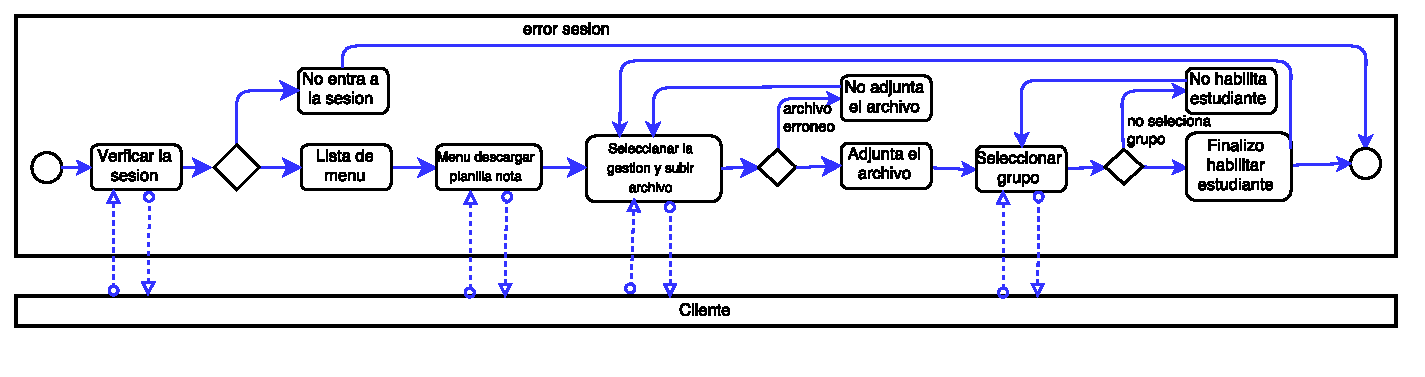
\includegraphics[width=0.8\textwidth]{flujoTrabajoSubir.pdf}
\captionsetup{justification=centering, margin=2cm}
\caption{Dise'no de flujo de trabajo de subir la planilla de notas, Fuente: Elaboraci'on propia}
\label{fig:FlujoTrabajoSubir2}
\end{figure}
\end{itemize}

\item \textbf{Crear un programa de flujo de trabajo}
\label{CrearFlujo}
el diagrama para crear un programa de flujo de trabajo es la uni'on de los servicios seleccionados anteriormente el dise'no de flujo de trabajo de descargar, modificar y adjuntar. Se representa en la siguientes figuras\ref{fig:FlujoTrabajoPlanilla} el crear un programa de flujo de trabajo. 
\begin{figure}[H]
\centering
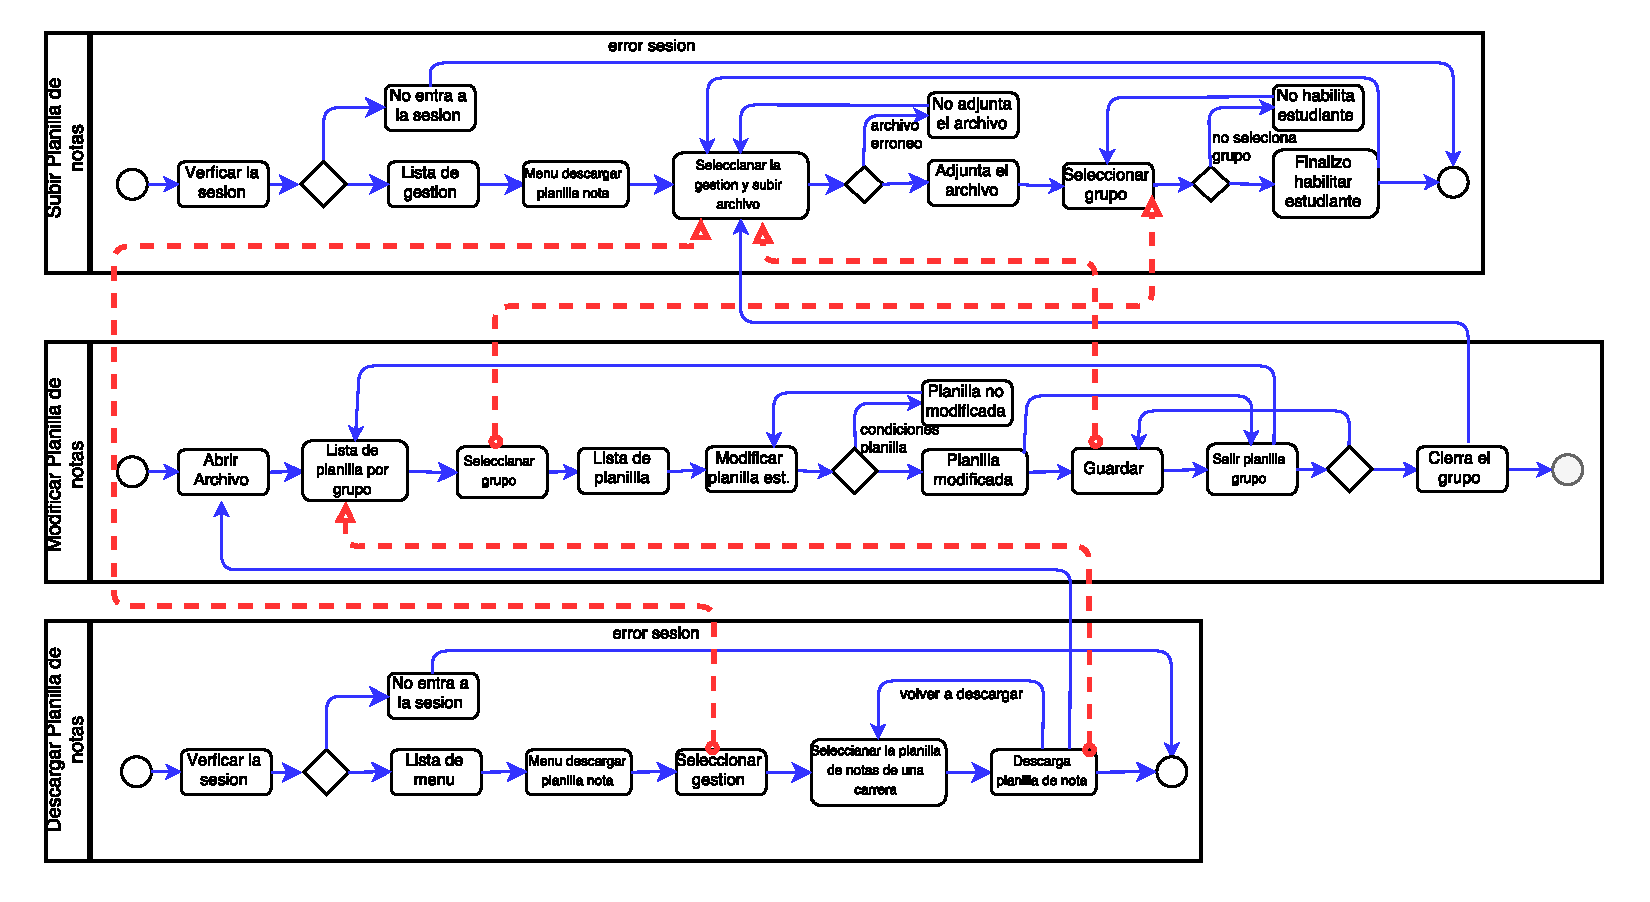
\includegraphics[width=1\textwidth]{flujoTrabajoPlanilla.pdf}
\captionsetup{justification=centering, margin=2cm}
\caption{Dise'no de flujo de trabajo planilla de notas, Fuente: Elaboraci'on propia}
\label{fig:FlujoTrabajoPlanilla}
\end{figure}
\end{itemize}
En la figura \ref{fig:FlujoTrabajoPlanilla} se representa los tres procesos, las flechas de punteada, es la comunicaci'on entre procesos y par'ametros que comparten entre ellos, para el desarrollo del servicio web.
%Hay que aumentar los datos del json.
%\subsection{El dise'no de unidad de datos de servicio} 
%El formato que se utiliza para intercambiar informaci'on, es un formato ligero conocido como \textbf{JSON} es representado en objetos y arreglos.// 

%La unidad de datos de la p'agina del SAGAA es definida con etiquetas y tiene la extensi'on sis, para el presente proyecto se ha utilizado para la estructura predefinida.//

%La unidad de datos sis, ha sido modificado para convertirlo en el formato json, y asi la aplicaci'on m'ovil pueda reconocerlo.

\section{Desarrollo de la implementaci'on del servicio}
Para el desarrollo de la implementaci'on del servicio se realiza a partir de la figura \ref{fig:FlujoTrabajoPlanilla}, el c'ual describe la selecci'on del servicio. La figura \ref{fig:FlujoTrabajoImplementar} representa el diagrama de flujo para la implementaci'on del servicio.


\begin{figure}[H]
\centering
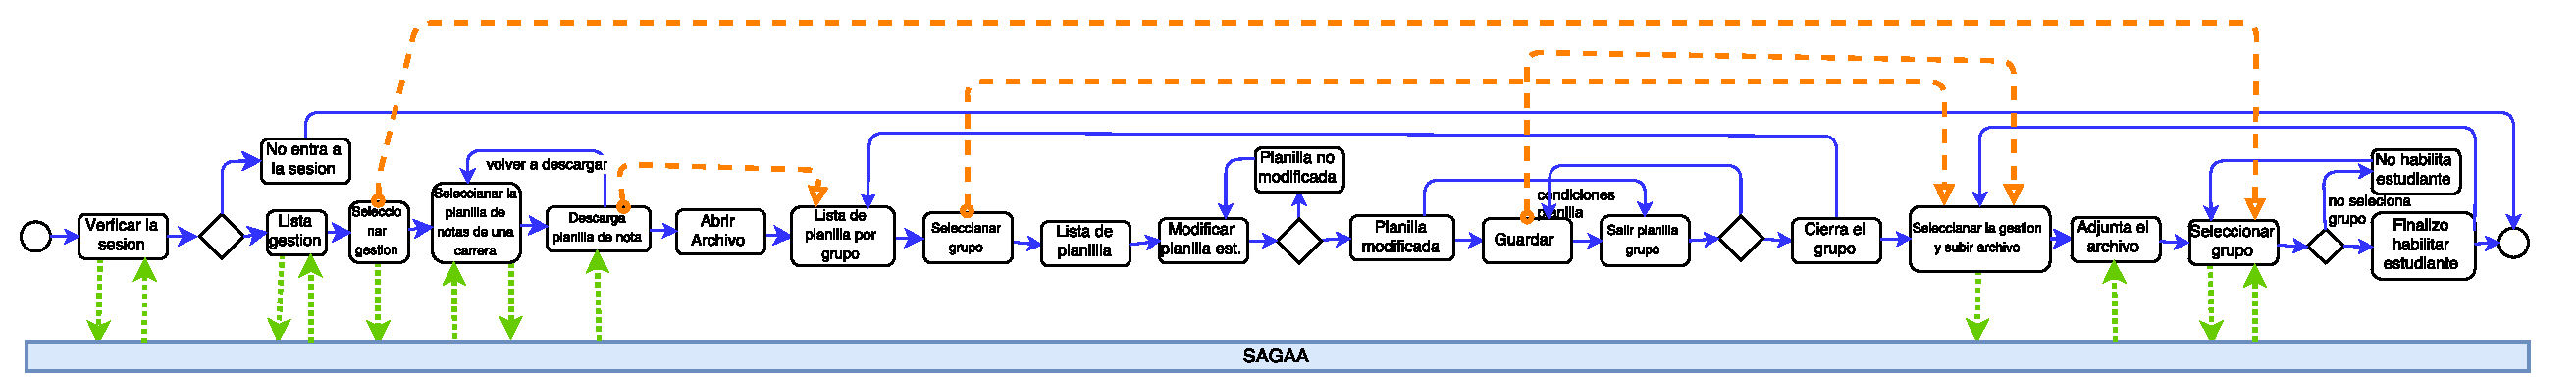
\includegraphics[width=1\textwidth]{flujoTrabajoImplementar.pdf}
\captionsetup{justification=centering, margin=2cm}
\caption{Dise'no de flujo de trabajo planilla de notas para la implementaci'on, Fuente: Elaboraci'on propia}
\label{fig:FlujoTrabajoImplementar}
\end{figure}

La figura \ref{fig:FlujoTrabajoImplementar} es la secuencia de proceso para el desarrollo del servicio web. Las lineas naranjas son par'ametros que comparten entre actividades.

\subsection{Herramientas y configuraci'on para la implementaci'ion del servicio}
Para el presente proyecto se ha utilizado el lenguaje de programaci'on de javascript y express es un framework de Nodejs. El express es una extensi'on de conecci'on con muchos m'etodos de la arquitectura de REST y intercambio de informaci'on a su disposici'on.

\begin{itemize}
\item \textbf{Arquitectura del framework Express} express utiliza la arquitectura de modelo, vista y controlador definida como MVC. 

\begin{figure}[H]
\centering
 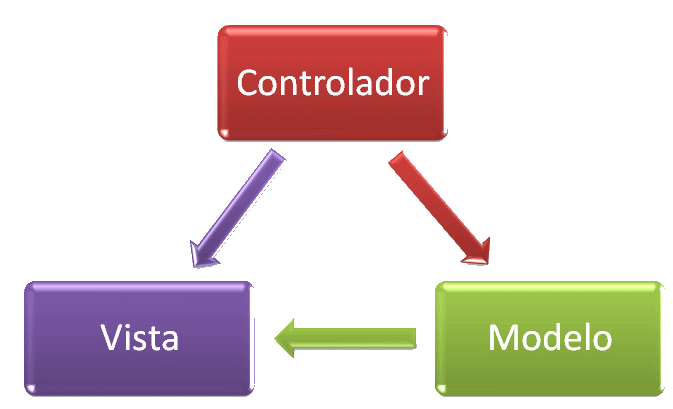
\includegraphics[width=0.4\textwidth]{arqExpress.png}
 \captionsetup{justification=centering,margin=2cm}
 \caption{Arquitectura de Express, adoptado para la realizaci'on del proyecto. Arquitectura de Express de \cite{Lopez2017}}
\end{figure}

Para el presente proyecto se ha implementado la parte del modelo para explicar la comunicaci'on del servicio web como se muestra  en la arquitectura de Nodejs en la figura \ref{fig:arqNodejs}..

\item\textbf{Arquitectura de Nodejs} utiliza la arquitectura orientado cliente/servidor.

\begin{figure}[H]
\centering
 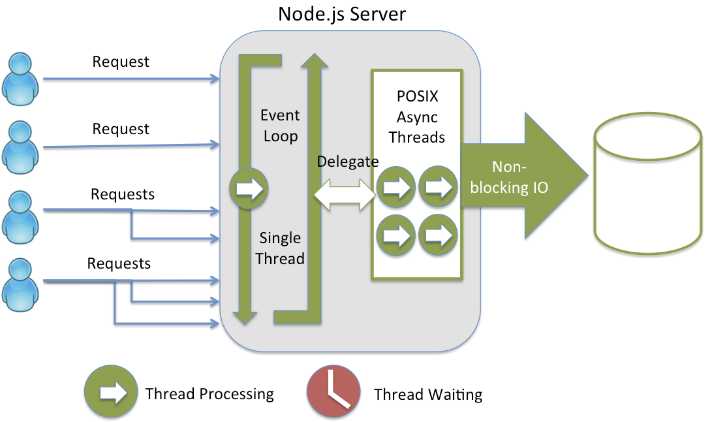
\includegraphics[width=0.6\textwidth]{arqNode.png}
 \captionsetup{justification=centering,margin=2cm}
 \caption{Arquitectura de NodeJs, adoptado para la realizaci'on del proyecto. Arquitectura de NodeJs de \cite{Munoz2013}}
 \label{fig:arqNodejs}
\end{figure}
En la arquitectura de Nodejs, analiza las peticiones de entrada y salida.
\end{itemize}

\subsection{Estructura del servicio web}
La estructura de servicio web utiliza la estructura de Ionic  tal como se ha mencionado anteriormente en el presente proyecto y  aumenta el archivo  server.js.
\begin{verbatim}
proyecto
    |--package.json (paquetes de plugin de NodeJS)
    |--plugins/ (Se guardan los plugins para el server)
    |--www/ (Código fuente principal)
    	|--archivo/ (guarda los archivos)
        |--js/ ( El código, Javascript de la aplicación)
            |--server.js
 \end{verbatim}

\subsection{Configuraci'on del servicio web}
Previamente se debe instalar node y npm para comenzar a realizar los siguientes comandos para configurar el servidor:

\begin{verbatim}
$ npm install -g express (instalar globalmente express)
$ touch server.js (crear el archivo server.js)
$ node server.js (ejecuta el server.js)
$ npm install nombre_plugins -g (instalar plugins necesarios para el proyecto)
\end{verbatim}
\subsection{Aplicar el servicio web en express}
Para la implementaci'on el servicio web se ha utilizado la herramienta de Curl, Cherrie y la cuenta de docente el cual ha sido proporcionada por la UPSI de la FCYT. Se ha utilizado el dise'no de flujo de trabajo de implementaci'on de planilla de notas de la figura  \ref{fig:FlujoTrabajoImplementar} el c'ual tiene los siguientes servicio web: 
\begin{itemize}
\item Verificar la sesi'on.
\item Listar la gesti'on. 
\item Seleccionar la gesti'on y devuelve la lista de las carreras.
\item Seleccionar la carrera de la planilla de notas para descargar planilla de notas. 
\item Filtrar y convertir la planilla de notas a unidades de datos de servicio json.
\item La planilla de notas con la unidad de datos modificados.
\item Crear una firma de clave para el servicio web.
\item Seleccionar la gesti'on y adjuntar planilla de notas modificada. 
\item Crear unidad de datos json.
\item Modificar los datos de la planilla de notas.
\item Configura el sesion de token.
\item Depende del anterior item seleccionar grupo para habilitar estudiante.
\end{itemize}
Cada servicio web es muy importante para lograr el objetivo general y se utilizan los datos del dise'no de interfaz l'ogico de la figura  \ref{fig:DisenoDescargar2} y el dise'no de interfaz l'ogica para adjuntar la planilla de notas de la figura \ref{fig:DisenoSubir} para realizar cada servicio web. Para mostar la implementaci'on del servicio web se explican las partes importantes a continuaci'on:
\begin{itemize}
\item \textit{Verificar la sesi'on} para verificar la sesion tenemos los siguientes datos: la direcci'on de url, el m'etodo que utiliza, los par'ametros y  agentes de autorizaci'on. Finalmente 'envia los datos mencionados a otra p'agina. 
\begin{verbatim}
var curl = new Curl(),
url  = 'http://pruebas.fcyt.umss.edu.bo/sagaa/login/loginP.php',
data = {
  'loginUsuario' : req.body.username,
  'claveUsuario' : req.body.password,
  'botonFormulario' : 'Ingresar'
};
curl.setOpt( Curl.option.URL, url );//direccion
curl.setOpt( Curl.option.FOLLOWLOCATION, true);//permite enviar a otra pagina
curl.setOpt( Curl.option.POST, 1);//metodo que utiliza
curl.setOpt( Curl.option.POSTFIELDS, data );//parametros 
curl.setOpt( Curl.option.HTTPHEADER, ['User-Agent: Mozilla/5.0',
'Content-Type: application/x-www-form-urlencoded'] );
// agentes de autorizacion
curl.setOpt( Curl.option.COOKIEFILE, 'pcb5r5tg8l1lbcjbqffr6hfm56'); 
// codigo de cookie de otra sesion, para obtener la sesion
curl.setOpt( Curl.option.COOKIEJAR, 'cookie.txt');
//guarda la cookie en el archivo txt
curl.on('end', function( statusCode, body, headers ) {
......
//respuesta de la comunicac'ion con el servidor del SAGAA
});
......
\end{verbatim}  
\item \textit{Seleccionar la gesti'on y adjuntar planilla de notas} para este servicio se conoce: la direcci'on de url, el m'etodo que utiliza, par'ametros encriptados, el httpheader para los agentes de autorizaci'on y la ubicaci'on de la planilla de notas para adjuntar.

\begin{verbatim}
....
dirA = '/home/geovanna/appSAGAA/appSAGAA/www/archivo/',
//ubicacion de la planilla de notas modificada
nameD = nombreAr,
idUsuario = usuarioId;
idGestion = gestionId;
url  = 'http://pruebas.fcyt.umss.edu.bo/sagaa/pre_academico/
subirNotasParcialesP.php';
curlS.setOpt( Curl.option.URL, url ); //direccion
curlS.setOpt( Curl.option.POST, 1); //metodo
curlS.setOpt( Curl.option.HTTPHEADER,['Connection: keep-alive',
'User-Agent: Mozilla/5.0','Content-Type: multipart/form-data;', 
'Cache-Control: max-age=0', 'Accept-Encoding: gzip, deflate']);
\\agentes de autorizacion
curlS.setOpt( Curl.option.HTTPPOST, [{name: 'idUsuario',
contents: idUsuario }, {name: 'idGestion', contents: idGestion },
{ name: 'archivoNotas', file: dirA + nameD, 
type: 'application/vnd.symbian.install'}, 
{ name: 'subirArchivo', contents: 'Subir Archivo'}]);
//estructura de parametros encriptados
curlS.setOpt( Curl.option.COOKIEFILE, 'cookie.txt');
//utiliza el cookie .txt para utilizar la sesion 
.......
\end{verbatim}
%\item \textit{Servicio web filtrar la planilla de notas} este servicio se encarga en recocer los datos de la planilla de notas al mostrar la planilla de notas y se elimina algunos datos por columna, para convertir a una unidad de datos de servicio.
%\begin{verbatim}
%.....
%   nuevoFile = data.split(/\n/);
%   inicio = nuevoFile[0];
%   nuevoFile.splice(nuevoFile[0],1);
%   fin = nuevoFile[nuevoFile.length-1];
%   nuevoFile.splice([nuevoFile.length-1],1);
%   nuevoFile.join('');
%.......
%\end{verbatim}
\item \textit{Crear unidad de datos json} la planilla de notas se convierte en datos json.
\begin{verbatim}
var parseString = require( 'xml2js' ).parseString;
.......
app.post('/detalle', function(req, res){
......
		parseString( fileS( body ), function( error, result ){....
         sisJson = result;
    .....});
......
}                   
\end{verbatim}
\item \textit{Modificar los datos de la planilla de notas} para modificar el archivo de planilla de notas primeramente buscar los dato modificado reemplazar el el archivo original.
\begin{verbatim}
\\ se busca del dato antiguo a partir del dato actual
function searchDato (pathlocal, arrayM){
   fs.readFileSync(pathlocal).toString().split('\n').forEach(recorriendo);
        function recorriendo(line, index, arr) {
        ......//verifica si son diferentes lo almacena en datoNuevo y datoAntiguo
            if(aux != arrayM[index]){
            ......
                if(arrayM[index] != '<normal>'){
                    if(arrayM[index]!='<me>'){
                        datoNuevo.push(arrayM[index]);
  					    datoAntiguo.push(line);
                    }
           ........
\end{verbatim}
\item \textit{Actualizar la planilla de datos,}
se  utiliza el plugin \textit{glob} el c'ual busca linea por linea el dato antiguo en la planilla de nota y lo remplaza por un dato modificado.
\begin{verbatim}
function addFile(file, antiguo, nuevo){
.....
glob(file, function(err, files) {
	if (err) { throw err; }
    	files.forEach(function(item, index, array) {
        	replace({
            	regex : antiguo,
                replacement : nuevo + '\r',
                paths : [item],
                recursive : true,
                silent : true
            });
         console.log('Remplaza por linea o  complete');
      });
........
\end{verbatim}

\item \textit{La configuraci'on la sesi'on de token}  a partir de la sesi'on y el token, se obtine la autentificaci'on para el servicio web.
\begin{verbatim}
var Base64 = require( 'js-base64' ).Base64;
var mySecretKey = "1234asdfLKKJH";
app.post('/datosU', function(req, res){
.......
 var cred64 = Base64.encode( data );
 var token = jwt.sign( data, mySecretKey );
 .....
 return res.status( statusCode ).json( token );
 ......
\end{verbatim}
\end{itemize}
Despu'es de concluir, con la implementaci'on del servicio web, se debe realizar las pruebas del servicio el cual se explica en el siguiente c'apitulo \ref{capituloseis}. 
\chapter{An'alisis y Dise'no de la aplicaci'on m'ovil}
\label{capituloseis}
En el presente c'apitulo se describe el desarrollo de la aplicaci'on m'ovil para cumplir con el objetivo general de \textit{proveer servicio a trav'es de una aplicaci'on m'ovil}. 
El desarrollo de la aplicaci'on m'ovil es la secuencia de pasos para ofrecer como resultado una aplicaci'on m'ovil.

Para el desarrollo de la aplicaci'on m'ovil se aplic'o el modelo iterativo incremental porque ha facilitado la comprensi'on y el analisis para el avanze de la aplicaci'on m'ovil en una serie de pasos hacia una soluci'on en diversas versiones hasta producir un aplicaci'ion adecuado\cite{Somerville2011}.

%\section{Estructura del Proyecto}
%\label{EstructuraIonic}
Para la estructura del proyecto utiliza el framework ionic con la  estructura de modelo, vista y controlador. Esta estructura se genera autom'aticamente al momento de crear el proyecto en carpetas y archivos para organizar el c'odigo. La estructura del framework se desarrolla en el anexo \ref{estructuraIonic}.


%\section{Implementaci'on del Proyecto}
%La implementaci'on se ha realizado seg'un los modulos \ref{ModuloMovil}, el dise'no de interfaz \ref{DisenoMovil} se han realizado en el c'apitulo \ref{capituloseis} y las herramientas de la aplicaci'on movil que se ha desarrollado en el c'apitulo \ref{capitulodos} los cuales  se dividen en las siguientes iteraciones.
Para el desarrollo de la aplicaci'on m'ovil se tiene informaci'on de la recolecci'on de datos del capitulo \ref{capitulotres} y la etapa de crear un nuevo servicio en el capitulo \ref{capitulocinco}.

\section{Primera iteraci'on}
En la primera iteraci'on se realizo la lista de requerimientos, el dise'no de interfaz  y la implementaci'on con datos estaticos.

\subsection{La primera etapa de analisis}
Como se ha mencionado anteriormente la informaci'on para la recoleccion de datos se obtuvo de los capitulos \ref{capitulotres} y \ref{capitulocinco}. El resultado es la siguiente lista de requerimientos.
%La especificaci'on de los requerimientos se tiene a partir del requerimiento del servicio en el c'apitulo \ref{capitulocinco} en la secci'on de requerimientos \ref{requerimientoServicio} y con la recolecci'on de datos del c'apitulo \ref{capitulotres} para cumplir el objetivos general de \textit{proveer los servicios de la aplicaci'ion SAGAA a trav'es de una aplicaci'on m'ovil}.
\textbf{Lista de requerimientos}
\begin{itemize}
\item Realizar Dise'no adaptativo.
\item Realizar la sesi'on.
\item Listar la gesti'on.
\item Listar carreras.
\item Mostrar los datos de la planilla de notas
\item Modificar la planilla de notas.
\item Almacenar la planilla de notas en el celular. 
\item Modificar planilla de notas sin internet.
\end{itemize}

Despu'es de concluir con la lista de requerimientos realizamos el dise'no para mostrar los datos de la planilla de notas.

\subsection{La primera etapa de dise'no interfaz}
\label{Doc:Interfaz}
El dise'no de interfaz representa el como se muestran los datos de la planilla de notas es por este motivo que tiene algunos datos repetidos como se muestra en la figura \ref{fig:IU}.
\begin{figure}[H]
\centering
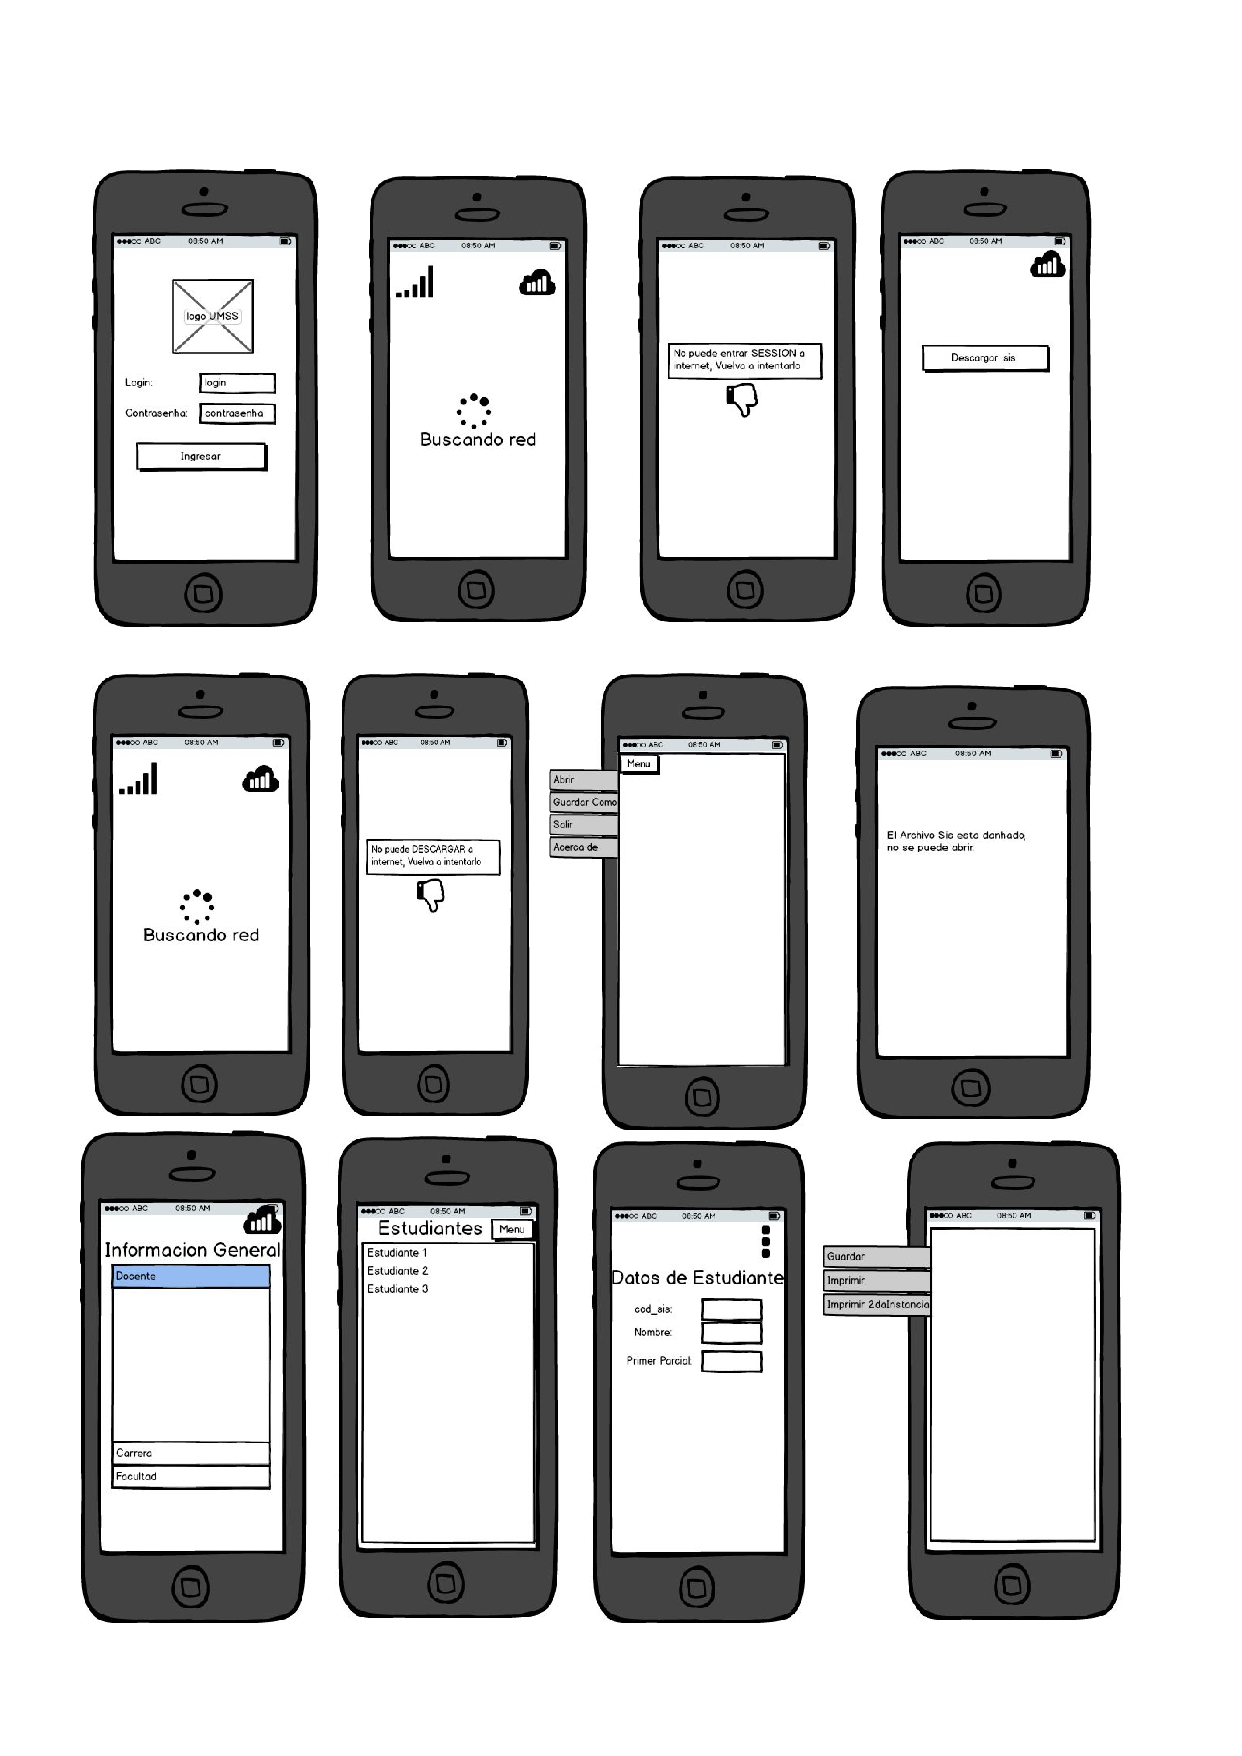
\includegraphics[width=0.6\textwidth]{mockupimprimir.pdf}
\captionsetup{justification=centering,margin=2cm}
\caption{Interfaz de Usuario primera etapa, Fuente: Elaboraci'on Propia}
\label{fig:IU}
\end{figure}

La interpretaci'on de la informaci'on de la planilla de notas es el primer paso para el desarrollo de la aplicaci'on m'ovil.

\subsection{La primera etapa de la implementaci'on}
Para la implementaci'on primeramente interpreta la informaci'on de la planilla de notas y gracias a la herramienta extra json y otros. Lo importante en la implementaci'on es la siguiente linea de c'odigo.
\begin{itemize}
\item Ordenar los datos del servicio web, se realizo en el archivo www/js/fileService.js en donde ordena los datos de la planilla de notas.

\begin{verbatim}
divFile : function(data , template){
if(template == 'informacion'){
   	return (((((data.pcd).head)[0]).info))[0];
	.........
},
crearBDInf : function(array){
	return  newBD = {
    	'fechaC ' : array[0],
        'fechaE'  : array[1],
        'codDoc' : array[2],
        'nomApeDoc' : array [3],
        ..........
    };
},
\end{verbatim}
\end{itemize}
  
\section{Segunda iteraci'on}
En la segunda etapa de iteraci'on se especifica el desarrolla de los m'odulos y el dise'no de la comunicaci'on con el servicio.

%\subsection{Dise'no de la comunicaci'on entre cliente y servicio}
%El dise'no de la comunicaci'on es una representaci'on abstracta de las solicitudes o peticiones que realiza la aplicaci'on m'ovil(cliente) y las respuestas del servicio web ofrece, como se muestra en la figura \ref{fig:DCS}.

%\begin{figure}[H]
%\centering
%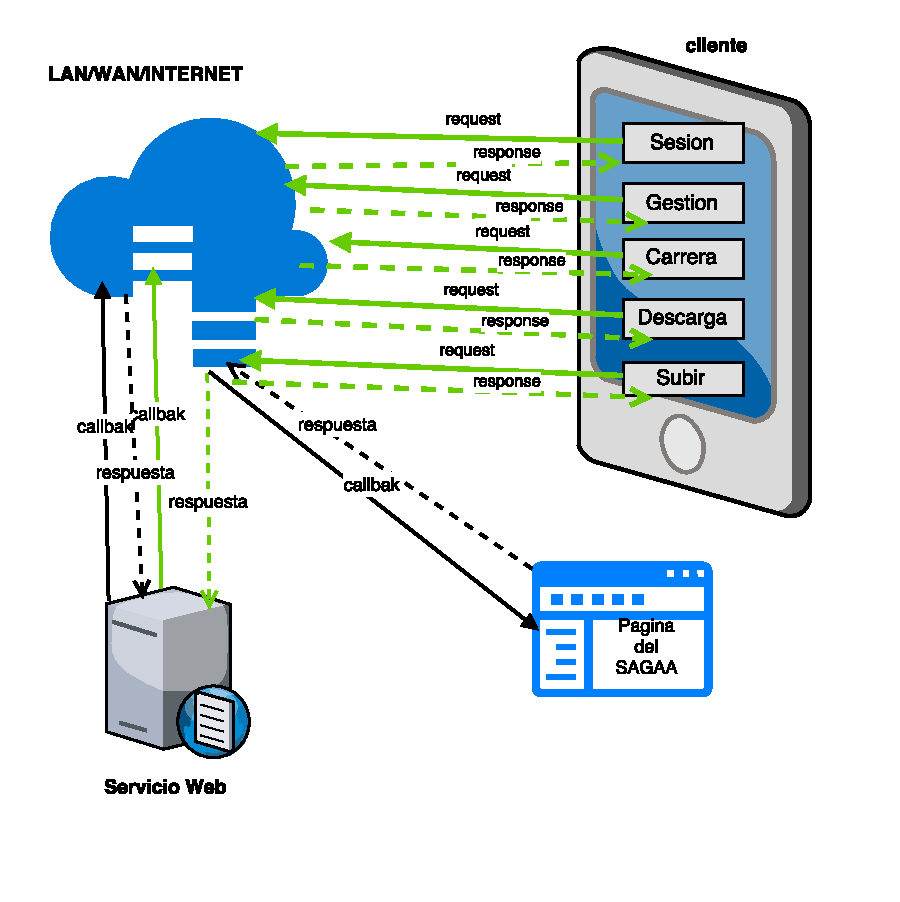
\includegraphics[width=0.4\textwidth]{comunicacionCS.pdf}
%\captionsetup{justification=centering,margin=2cm}
%\caption{Dise'no de comunicaci'on entre el cliente y servicio web Fuente: Elaboraci'on Propia}
%\label{fig:DCS}
%\end{figure}

%La implementaci'on es el proceso de realizar el dise'no como una aplicaci'on movil, que se explica a continuaci'on.

\subsection{La segunda etapa del analisis}
\label{ModuloMovil}
A partir de la lista de requerimientos se realiza el an'alisis de la segunda etapa, en esta etapa a continuaci'on se realiza la lista de m'odulos y subm'odulos las cuales son: 

\subsection{Lista de m'odulos del proyecto}
\begin{enumerate}
\item Mostrar la planilla de notas.
\item Modificar la planilla de notas.
\item Obtener datos del servicio web.
\item Guardar la planilla de notas en el servicio web.
\end{enumerate}
     
\subsection{ Lista de submodulo del proyecto}
\begin{enumerate}
\item Mostrar la planilla de notas.
\begin{itemize}
\item Crear la sesi'on para mostrar la planilla de notas.
\item Seleccionar la planilla de notas seg'un la gesti'on.
\item Seleccionar la planilla de notas seg'un la carrera.
\end{itemize}

\item Modificar la planilla de notas.
\begin{itemize}
\item Mostrar la planilla de notas ordenado por grupo.
\item Modificar la planilla de notas por grupo.
\end{itemize}

\item Obtener datos del servicio web.
\begin{itemize}
\item Verificar la sincronizaci'on con el servicio web.
\item Si no tiene sincronizaci'on con el servicio web generar un repositorio de la planilla de notas local.
\end{itemize}

\item Guardar la planilla de notas en el servicio web.
\begin{itemize}
\item Enviar la planilla de notas al servicio web.
\item Verificar la sincronizaci'on con el servicio web para guardar la planilla de notas.
\end{itemize}
\end{enumerate}

Una vez concluido con la lista de m'odulos se determina el dise'no de interfaz para la aplicaci'on m'ovil.

\subsection{ La segunda etapa del Dise'no de interfaz }
\label{DisenoMovil}
El dise'no de interfaz es la etapa de proceso donde las m'odulos y subm'odulos se interlazan con la implementaci'on.
%Para cumplir con el objetivo especifico \ref{sec:oe}  y se utilizan las herramienta de wireframe, las cuales son:

El segundo dise'no se ha modificado con las observaciones del primer intento y se toma en cuenta el servicio. El dise'no se presenta en la en la siguiente figura \ref{fig:IU2}.

\begin{figure}[H]
\centering
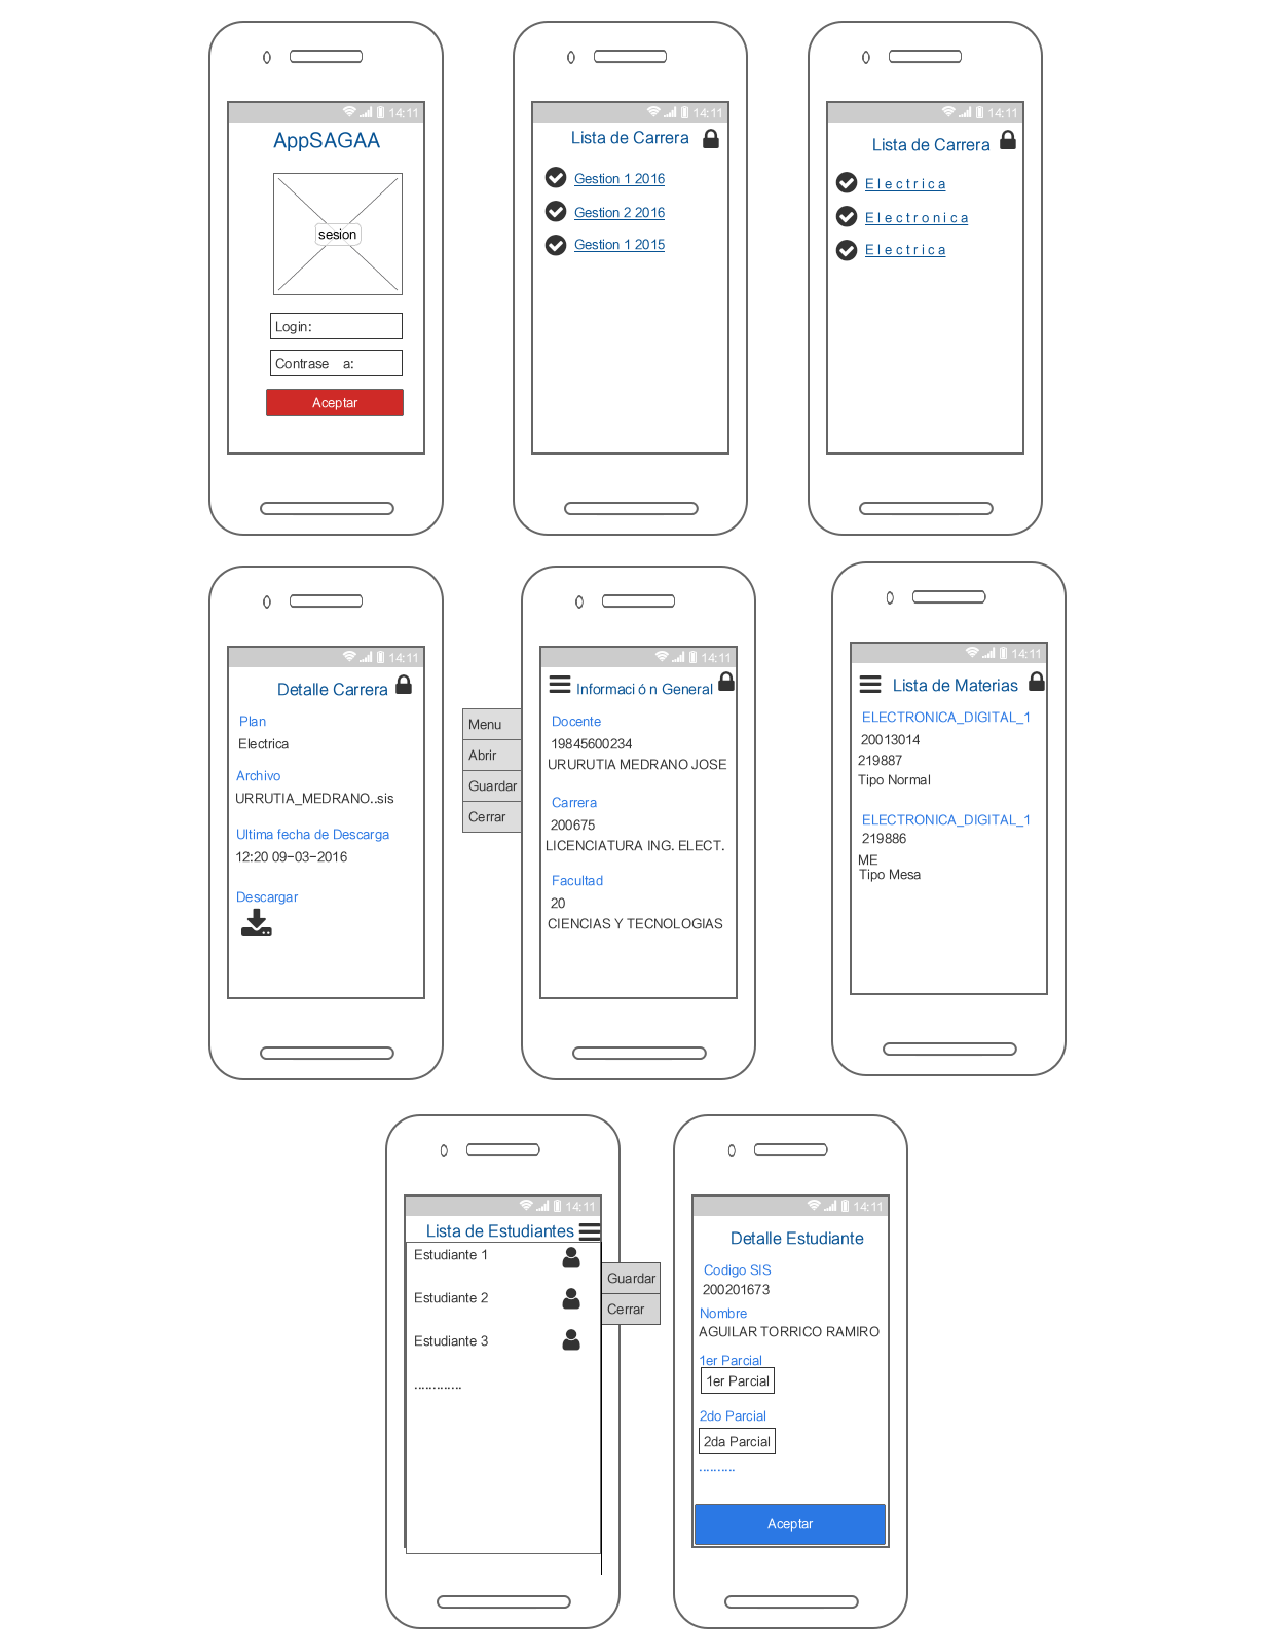
\includegraphics[width=0.5\textwidth]{Interfaz.pdf}
\captionsetup{justification=centering, margin=2cm}
\caption{Interfaz de Usuario representado en mockups, Fuente: Elaboraci'on Propia}
\label{fig:IU2}
\end{figure}
\end{enumerate}
  
Una vez concluido con el dise'no de interfaz, conocido como el esquema de pantallas, se desarrolla la implementaci'on.
%, se realiza el dise'no de la comunicaci'on entre cliente y el servicio web.

\subsection{La segunda etapa de la Implementaci'on}
En esta etapa de implementaci'on se desarrolla la comunicaci'on con el servicio, la sesi'on a traves del servicio, solicitar informaci'on del servicio y otros. En los siguientes indicen se explican algunos de la implementaci'on.

\begin{itemize}
\item Solicitud de la planilla de notas al servicio web se realizo en el archivo www/js/fileFactory.js

\begin{verbatim}
sisFactory.posDataDetalle = function(carrera){
.......
 $http.post(urlBase+'/detalle', descargarD, {skipAuthorization : false}, conf).
 success(function(data) {
 .......
 }; 
\end{verbatim}

\item La configuraci'on para enviar el jwt en la cabecera de la petici'on se crea un nuevo interceptor el c'ual se guarda localmente se implemento en el archivo www/app.js

\begin{verbatim}
...
.config(function($stateProvider, $urlRouterProvider, $authProvider, 
$httpProvider, jwtInterceptorProvider, jwtOptionsProvider) { 
.....
 jwtOptionsProvider.config({
 	//IP de la maquina actual 
	 whiteListedDomains: ['localhost', '172.20.10.3'] 
	 tokenGetter: function(options, jwtHelper){
	 var token = localStorage.getItem('id_token');
}});
	//metodo para enviar un json web token
$httpProvider.interceptors.push('jwtInterceptor');
......
\end{verbatim}
\item La configuraci'on para conectar la aplicaci'on m'ovil al servicio web se ha desarrollado en el archivo www/js/fileFactory.js: 
\begin{verbatim}
//IP de la maquina donde se encuentra el server.js
var urlBase = 'http://172.20.10.3:8080';
var conf = {
	headers : {
	'Access-Control-Allow-Origin' : '*',
    'Access-Control-Allow-Methods' : 'POST, GET, OPTIONS, PUT',
    'Content-Type': 'application/jsonr',
    'Accept': 'application/json'
    } 
};
\end{verbatim}
\end{itemize}

\section{Tercera iteraci'on}
En la tercera iteraci'on se desarrolla el modificar la planilla de notas sin conexi'on a internet de la aplicaci'on movil, almacenar informaci'on en la aplicaci'on m'ovil y otros. En este iteraci'on se ha desarrollado el dise'no responsive para la aplicaci'on, el cual se explican en el c'apitulo \ref{capituloocho}.
\subsection{La tercera etapa de dise'no}
En la tercera etapa de dise'no se representa la comunicaci'on entre la aplicaci'on movil y la base de datos como se muestra en la siguiente figura \ref{fig:DO}. Como es una base de datos no sql es por este motivo que se guardan los datos como documentos por lo tanto no se tiene un dise'no de base de datos.

\begin{figure}[H]
\centering
\includegraphics[width=0.3\textwidth]{DisenoOffline}
\captionsetup{justification=centering, margin=2cm}
\caption{Dise'no aplicaci'on movil y base de datos, Fuente: Elaboraci'on Propia}
\label{fig:DO}
\end{figure}

\subsection{El tercer etapa de la implementaci'on}
Para modificar la planilla de notas, sin conexi'on a internet, anteriormente ha debido crear su sesi'on y descargar la planilla de notas se utiliza localmente como se muestran a continuaci'on:
\begin{itemize}
\item Se utiliza el pouchdb y websql para crear, actualizar y modificar la base de datos se realizan en el archivo www/js/fileService.js.
\begin{verbatim}
.service('SagaaService', function($q) {
......
_db = new PouchDB('sagaa', { adapter: 'websql' }, 
 { skip_setup: true });//crear base de datos
 ......
  return $q.when( _db.post( sagaa));//añadir
  ......
  return $q.when(_db.put(sagaa));//actualizar
   .......
\end{verbatim}
\item Se guardan las solicitudes del servicio que tienen alg'un problema con la conecci'on o respuestas err'oneas, esto se ha realizado en el archivo app.js.
\begin{verbatim}
.....
//crea un interceptor
$httpProvider.interceptors.push('myInterceptor');
.....
//crear un interceptor
//crear metodo, para conocer la respuesta o la peticion
var interceptor = function ($q, logHttp) {
return {
  responseError: function(rejection) {
  logHttp.push(rejection.config);
  ......
  return $q.reject(rejection);
  ......}
}
\end{verbatim}
\item Guardar y verificar las peticiones al servicio se ha realizado en el fileService.js  
\begin{verbatim}
.service('myInterceptor', function($q, $timeout, logHttp){
return { 
	'request': function(config){ 
	......//guardamos la peticion sin error
	logHttp.push(config);
	.....
	'requestError': function(rejection){
	//guarda la peticion con error, 
	window.localStorage.setItem('id_request', data);
	......// lo mismo realiza en la respuesta con error
	.......
.service('logHttp', function($q) {
	push: function(config) {
	requestsConfig = config;
.............
\end{verbatim}
\end{itemize}

%desde aqui comienza
%En este c'apitulo se utilizan los datos obtenidos, del c'apitulo \ref{capituloseis} y se explican las herramientas que se utilizan para la implementaci'on de la aplicacion m'ovil y el desarrollo del mismo.



%\chapter{Implementaci'on de la aplicaci'on m'ovil}
\label{capitulosiete}
En este c'apitulo se utilizan los datos obtenidos, del c'apitulo \ref{capituloseis} y se explican las herramientas que se utilizan para la implementaci'on de la aplicacion m'ovil y el desarrollo del mismo.
\section{Herramienta  y configuraci'on de la aplicaci'on m'ovil} 
\label{HerramientaMovil}
Para el desarrollo de la aplicaci'on m'ovil, se ha utilizado el framework ionic.
Ionic es de c'odigo libre y se basa en librer'ias orientadas 'unicamente a aplicaciones de dispositivos m'oviles. Tambi'en se enfocan a desarrollo de aplicaciones h'ibridas, construida con HTML3, CSS3 y Javascript se construye p'aginas web, se ejecutan dentro de un navegador, el c'ual aportan para ejecutar, en diferentes plataformas: android, iOS, windowsPhone, etc. Utiliza el framework de angular y es integrado con cordova, el c'ual permite el acceso a las caracter'isticas nativas del dispositivo.El framework de angular, utiliza la arquitectura de patrones de modelo, vistas y controladores, es la base para la arquitectura de ionic, se muestra en la figura \ref{fig:Ionic}.

%figura Arquitectura de Ionic
\begin{figure}[H]
\centering
 \includegraphics[width=0.5\textwidth]{arqIonic.png}
 \captionsetup{justification=centering,margin=2cm}
 \caption{Arquitectura de Ionic, adoptado para la realizac'ion del proyecto Fuente: \cite{Gallego}}
\label{fig:Ionic}
\end{figure}

Para explicar la arquitectura de ionic se tiene diferentes tipos de componentes, que se explican a continuaci'on:

\begin{enumerate}
\item \textbf{Config y routes:} es el archivo app.js, donde se realiza la configuraci'on y las rutas, que permiten enlazar el controlador con la la interfaz de usuario correspondiente.
\item \textbf{Controller:} es el archivo controller.js,  realiza la comunicaci'on a trav'es de la variable scope entre la interfaz de usuario y los servicios de los archivos services.js o factory.js.
\item \textbf{Directives:} es el archivo directive.js permite crear y usar componentes con aspectos y comportamiento.
\item \textbf{Factory:} son los archivo service.js y factory.js, son modelo de datos que ayudan a obtener los datos, del servicio web.
\item \textbf{View:} son los archivos html que contienen la descripci'on visual y obtiene los datos a mostrar el scope.
\end{enumerate}

\subsection{Estructura del Proyecto}
\label{EstructuraIonic}
El framework ionic, utiliza la estructura de modelo, vista y controlador del proyecto, el c'ual se genera autom'aticamente al momento de crear el proyecto en carpetas y archivos, para organizar el c'odigo en los siguientes archivos:

\begin{verbatim}
 proyecto
    |--bower.json (Lista de dependencias y paquetes de Bower)
    |--.bowerrc
    |--config.xml (Contiene la configuracion de la plataforma)
    |--.editorconfig
    |--.gitignore
    |--gulpfile.js (Lista de tareas de Gulp)
    |--hooks/ (Anade scripts que producen eventos)
    |--ionic.project (Configuracion de Ionic)
    |--package.json (Dependencias y paquetes de NodeJS)
    |--platforms/ (Codigo plataformas para compilar)
    |--plugins/ (Plugins o modulos de aplicacion)
    |--resources/ (Recursos plataforma concreta)
    |--scss/ ( Codigo SCSS compilado en www/css)
    |--www/ (Codigo fuente principal)
        |--css/ (Estilos que se usa en la aplicacion)
        |--img/ (Imagenes de nuestro proyecto)
        |--index.html (Fichero principal, cargamos necesario)
        |--js/ (El codigo, Javascript de la aplicacion)
            |--app.js 
            |--controllers.js
            |--directive.js
            |--factory.js
            |--filter.js
            |--service.js
        |--lib (Librerias, del codigo)
        |--templates/(Vistas de la aplicacion)
\end{verbatim}

\subsection{Configuraci'on del proyecto}

Para, el presente proyecto se utiliza, el interprete de linea de comando denominado (cli) de ionic, el c'ual, tiene los siguientes comandos:

\begin{verbatim}
$ ionic start appSAGAA sidemenu (crea proyecto)
$ ionic platform add android (añadir la plataforma)
$ ionic build android (compilar el proyecto)
$ ionic run android (ejecutar el proyecto)
$ ionic serve (ejecutar, compila y muestra en el navegador )
\end{verbatim}

Se crea autom'aticamente, la carpeta de appSAGAA con  la estructura  de la figura \ref{EstructuraIonic} y el men'u sidemenu por defecto.

\section{Herramientas Extras}
\label{HerramientasExtras}
Para el presente proyecto se ha utilizado algunas herramientas extras como ser: cordova, pouchDB, json web token y localstorage.

\subsection{Framework cordova}
Cordova es un framework de c'odigo libre, para desarrollo m'ovil, que nos permite usar est'andares de tecnolog'ias web como HTML5,CSS3 y Javascript. Se basa en  los enlaces de API's compatibles para acceder a las capacidades del dispositivos como sensores, red, etc. En la figura \ref{fig:arqCordova} se muestra arquitectura de Cordova.

\begin{figure}[H]
\centering
\includegraphics[width=0.3\textwidth]{arqCord.png}
\captionsetup{justification=centering,margin=2cm}
\caption{Arquitectura de Cordova, adoptado para la realizac'ion del proyecto Fuente: \cite{Cantabriatic}}
\label{fig:arqCordova}
\end{figure}

Para el presente proyecto se utiliza cordova, se agrega su librer'ia al proyecto y se instala el plugin necesario.

\subsection{PouchDB}
Es una capa de otras base de datos, se almacenan en el navegador, permite guardar los datos a lado del cliente,  es desarrollado en JavaScript. La estructura de pouchdb, se representa en la figura \ref{fig:pouchDB}. 
\begin{figure}[H]
\centering
\includegraphics[width=0.3\textwidth]{pouchDB.png}
\captionsetup{justification=centering,margin=2cm}
\caption{Adaptadores de PouchDB, adoptado para la realizac'ion del proyecto Fuente: \cite{Pouch}}
\label{fig:pouchDB}
\end{figure}

Para el presente proyecto se ha utilizado la capa del adaptador de websql, se explica a continuaci'on.
\subsection{Base de datos websql}
Es una herramienta para internet e intranets, facilita el acceso a base de datos relacionada con la web. Integra la tecnolog'ia  del cliente y abre la sybase, el c'ual permite que los datos de la fuente, se han incorporadas din'amicamente en la p'agina web, se representa en la figura \ref{fig:websql}.
\begin{figure}[H]
\centering
\includegraphics[width=0.6\textwidth]{websql.pdf}
\captionsetup{justification=centering,margin=2cm}
\caption{Base de datos websql, adoptado para la realizac'ion del proyecto Fuente: \cite{Websql1997}}
\label{fig:websql}
\end{figure}

\subsection{Almacenamiento local}
Es una propiedad de HTML5 web de almacenamiento, que permiten almacenar datos en nuestro navegador web denominada localstorage.
Guarda la informaci'on que permanece almacenada por tiempo indefinido, sin importar que el navegador se cierre. Tiene las siguientes caracteristicas, almacenar entre 5MB y 10MB de informaci'on, est'a almacenada en la computadora del cliente y no es enviado en cada petici'on del servidor, previene perdidas de informaci'on cuando se desconecta de la red y la informaci'on es guardada por dominio web \cite{Cardenas2015}.
\subsection{Interceptor}                                                                                                                                                                                                                                              
El interceptor utiliza el servicio de \textit{http}, el c'ual permite la comunicaci'on con el servidor y captura cada petici'on y lo manipula a trav'es del \textit{httpProvider}, es el que registra el contenedor del arreglos y ofrece un servicio regulador.
\subsection{Json web token}
Json web token es un m'etodo abierto y est'andar para representar las  reclamaciones de forma segura, entre dos partes que comparten informaci'on y autentificaci'on moderna, de m'ovil. El c'ual tiene una estructura representada en la figura \ref{fig:jwt}.
\begin{figure}[H]
\centering
\includegraphics[width=0.6\textwidth]{jwt.pdf}
\captionsetup{justification=centering,margin=2cm}
\caption{Json web token, adoptado para la realizac'ion del proyecto Fuente: Elaboraci'on propia}
\label{fig:jwt}
\end{figure}

Estos son las herramientas extras, se utilizan para el presente proyecto, los c'uales son compatibles con el framework ionic.

\section{Implementaci'on del Proyecto}
Para la implementaci'on del presente proyecto, se ha utilizado las herramientas \ref{HerramientaMovil} y las herramientas extras \ref{HerramientasExtras}, se ha realizado seg'un los modulos \ref{ModuloMovil}, el dise'no de interfaz \ref{DisenoMovil} que se han realizado en el c'apitulo \ref{capituloseis}
dividido en los siguientes intento.

\subsection{El primer intento o iteraci'on la configuraci'on para conectarse al servicio web}
Configurar la aplicaci'on m'ovil para solicitar la planilla de notas al servicio web, se explican los puntos importantes:

\begin{enumerate}
\item La configuraci'on para conectar la aplicaci'on m'ovil al servicio web, se realizo en el archivo www/js/fileFactory.js: 
\begin{verbatim}
//IP de la maquina donde se encuentra el server.js
var urlBase = 'http://172.20.10.3:8080';
var conf = {
	headers : {
	'Access-Control-Allow-Origin' : '*',
    'Access-Control-Allow-Methods' : 'POST, GET, OPTIONS, PUT',
    'Content-Type': 'application/jsonr',
    'Accept': 'application/json'
    } 
};
\end{verbatim}

\item Solicitud de la planilla de notas al servicio web, se realizo en el archivo www/js/fileFactory.js

\begin{verbatim}
sisFactory.posDataDetalle = function(carrera){
.......
 $http.post(urlBase+'/detalle', descargarD, {skipAuthorization : false}, conf).
 success(function(data) {
 .......
 }; 
\end{verbatim}

\item Ordenar los datos del servicio web, se realizo en el archivo www/js/fileService.js.

\begin{verbatim}
divFile : function(data , template){
if(template == 'informacion'){
   	return (((((data.pcd).head)[0]).info))[0];
	.........
},
crearBDInf : function(array){
	return  newBD = {
    	'fechaC ' : array[0],
        'fecgaE'  : array[1],
        'codDoc' : array[2],
        'nomApeDoc' : array [3],
        ..........
    };
},
\end{verbatim}
\end{enumerate}
\subsection{El segundo intento o iteraci'on la sesi'on}
Para asegurar la sesi'on el servicio web, 'envia en la cabecera la llave denominado jwt, el c'ual se explica la implementaci'on en las partes importante a continuaci'on:
\begin{enumerate}
\item La configuraci'on para enviar el jwt en la cabecera de la petici'on, se crea el interceptor, el c'ual se guarda localmente, se realizo en el archivo www/app.js

\begin{verbatim}
...
.config(function($stateProvider, $urlRouterProvider, $authProvider, 
$httpProvider, jwtInterceptorProvider, jwtOptionsProvider) { 
.....
 jwtOptionsProvider.config({
 	//IP de la maquina actual 
	 whiteListedDomains: ['localhost', '172.20.10.3'] 
	 tokenGetter: function(options, jwtHelper){
	 var token = localStorage.getItem('id_token');
}});
	//metodo para enviar un json web token
$httpProvider.interceptors.push('jwtInterceptor');
......
\end{verbatim}
\end{enumerate}

\subsection{El tercer intento o iteraci'on trabajar sin el servicio web}
Para modificar la planilla de notas, sin conexi'on a internet, anteriormente ha debido crear su sesi'on y descargar la planilla que utilizan localmente, se muestra los puntos mas importantes:
\begin{enumerate}
\item Se utiliza el pouchdb y websql para crear, actualizar y modificar la base de datos, se realizo en el archivo www/js/fileService.js.
\begin{verbatim}
.service('SagaaService', function($q) {
......
_db = new PouchDB('sagaa', { adapter: 'websql' }, 
 { skip_setup: true });//crear base de datos
 ......
  return $q.when( _db.post( sagaa));//añadir
  ......
  return $q.when(_db.put(sagaa));//actualizar
   .......
\end{verbatim}
\item Se guardan las solicitudes al servicio web, que tienen alg'un problema con la conecci'on, se realizo en el archivo app.js.
\begin{verbatim}
.....
//crea un interceptor
$httpProvider.interceptors.push('myInterceptor');
.....
//crear un interceptor
//crear metodo, para conocer la respuesta o la peticion
var interceptor = function ($q, logHttp) {
return {
  responseError: function(rejection) {
  logHttp.push(rejection.config);
  ......
  return $q.reject(rejection);
  ......}
}
\end{verbatim}
\item Guardar y verificar las peticiones, se realizo en el fileService.js  
\begin{verbatim}
.service('myInterceptor', function($q, $timeout, logHttp){
return { 
	'request': function(config){ 
	......//guardamos la peticion sin error
	logHttp.push(config);
	.....
	'requestError': function(rejection){
	//guarda la peticion con error, 
	window.localStorage.setItem('id_request', data);
	......// lo mismo realiza en la respuesta con error
	.......
.service('logHttp', function($q) {
	push: function(config) {
	requestsConfig = config;
.............
\end{verbatim}
\end{enumerate}

\chapter{Implementaci'on del dise'no adaptativo para la aplicaci'on m'ovil}
\label{capituloocho}
En este capitulo se explica el analisis, dise'no e implementaci'on del dise'no adaptativo para la aplicaci'on m'ovil con la proposito de cumplir el objetivo especifico \textit{Proveer un dise'no adaptativo para la aplicaci'on m'ovil} como se muestra en c'apitulo \ref{capitulouno} en la secci'on \ref{sec:oe}.

%Como se ha mencionado en el c'apitulo \ref{capitulouno} en la secci'on del objetivo especifico \ref{sec:oe}, se tiene en el presente c'apitulo como objetivo presentar el responsive de la aplicaci'on m'ovil, a trav'es de los componentes de CSS del framework ionic, que utiliza cuadrillas para proporcionar una soluci'on a la variedad  de resoluci'on de diferentes dispositivos m'oviles inteligentes y tablets.

\section{Dise'no adaptativo o responsive}
El dise'no adaptativo tiene la filosof'ia de \textit{Responsive Web Design (RWD\footnote{RWD- Dise'no web responsive})} establecida por Steven Champeon (2003) el propone solucionar los problemas de dise'no para los dispositivos u orientaci'on. Este problema se refiere al contenido para adaptar a los dispositivos creando una soluci'on 'unica.\cite{Adrian2012}. 

En este proyecto se ha utilizado para verificar la aplicaci'on m'ovil en dispositivos de diferentes tama'nos de resoluci'on de pantalla. Dicha aplicaci'on se ha desarrollado en el framework Ionic. A continuaci'on se explica el componente de Ionic para desarrollar un dise'no adaptativo.
%desarrollado una aplicaci'on m'ovil h'ibrida para el sistema operativo de android, el c'ual tiene dispositivos en diferentes tama'no de resoluci'on de pantalla. El desarrollo de la implementaci'on se ha utilizado el framework ionic.

\section{Componentes de Ionic}
El componente de Ionic el c'ual tiene un sistema cuadr'iculada con el est'andar de CSS\footnote{CSS- Hojas de estilo en cascada} y modulo flexible de la caja de layout seg'un su p'agina oficial. 
%Los dispositivos son compatibles con el framework ionic soportan la herramienta de \textit{flexbox} utiliza la herramienta grid. 
Las caracter'isticas de componentes de CSS esta representada en la figura \ref{fig:GridI}.
\begin{figure}[H]
\centering
\includegraphics[width=0.6\textwidth]{gridIonic.pdf}
\captionsetup{justification=centering,margin=2cm}
\caption{Componente de CSS de ionic, Fuente: P'agina oficial}
\label{fig:GridI}
\end{figure}

\section{Implementaci'on de responsive}
Con el objetivo de implementar el responsive se ha utilizado el flexbox el c'ual se encarga de realizar los cortes de las cuadrillas en la siguiente linea de c'odigo.
\begin{verbatim}
  <div class="row responsive-sm  responsive-md">
  //El responsive-sm reduce la fila para visualizar de forma horizontal para movil
  //El responsive-md se amplia la columna de forma vertical para la tablets
  <div class="col col-33">
  \\ El col-33 define el 33% de la resolucion de la pantalla
\end{verbatim}


\section{Visualizaci'on del contenido con flexbox}
La visualizaci'on del contenido con flexbox es el resultado de la implementaci'on del responsive las diferencia se observa en la siguiente figura \ref{fig:GridI1}
%La visualizacion  se aplica el componente grid responsive de ionic, el c'ual nos ayuda en definir las filas, columnas  responsive grid donde la columna se adapta al 'area. En la siguiente figura se muestra la diferencia.
\begin{figure}[H]
\centering
\includegraphics[width=0.2\textwidth]{gridIonic1.png}
\captionsetup{justification=centering,margin=2cm}
\caption{Visualizacion de contenido vertical en la tablet, Fuente: Elaboraci'on propia}
\label{fig:GridI1}
\end{figure}
 
En la figura \ref{fig:GridI1} se muestra la tablet con orientaci'on vertical donde las imagenes se acomodan en forma vertical y secuencial.

\begin{figure}[H]
\centering
\includegraphics[width=0.6\textwidth]{gridIonic2.png}
\captionsetup{justification=centering,margin=2cm}
\caption{Visualizaci'on de contenido horizontal en la tablet, Fuente: Elaboraci'on propia}
\label{fig:GridI2} 
\end{figure}
La representaci'on de la tablet en orientaci'on horizontal y los datos se acomodan de 3 columnas debido a la resoluci'on de la pantalla como se muestra en la \ref{fig:GridI2}.
\chapter{Pruebas del servicio web a trav'es de la aplicaci'on m'ovil} 
\label{capitulonueve}
Esta c'apitulo \ref{capitulonueve} se verifica las funciones de la etapa de prueba de servicio web este es una combinaci'on entre servicios. Es la etapa de verificar que nuestro servicio web brinde servicio a la aplicaci'on m'ovil. En el c'apitulo \ref{capituloseis} la aplicaci'on m'ovil realiza peticiones al servicio web y en el c'apitulo \ref{capitulocinco} el servicio web ofrece servicios de la p'agina del SAGAA. Uniendolos se empieza a validar el servicios web como se explica mas adelante.

\section{La etapa de prueba de descargar la planilla de notas con el servicio}
La etapa de prueba entre descargar la planilla de notas y el servicio se realiza en la funcionalidad de descargar la planilla de notas en los siguientes procesos: realizar la sesi'on del docente, listar la gesti'on, seleccionar la gesti'on, listar las carreras y selecci'onar la carrera para descargar la planilla de notas. A continuaci'on se muestra algunos de los servicios para descargar la planilla de notas.
\subsection{Prueba de sesi'on}
\label{Sesion}
La prueba de la sesi'on en el servicio se realiza en el 
desarrollo la sesi'on, al empezar la aplicaci'on m'ovil 'envian los datos al servicio el c'ual se encarga de enviar los par'ametros a la p'agina del SAGAA. Como se muestra en la figura \ref{fig:movilSesion} de la aplicaci'on m'ovil que 'envia los datos al servicio y en la figura \ref{fig:servicioSesion} es la ejecuci'on del servicio en el c'ual se muestra la conecci'on y la respuesta con la p'agina de SAGAA y obtiene la respuesta \textit{OK}. 
\begin{figure}[H]
\begin{minipage}{0.48\textwidth}
\centering
\includegraphics[width=.4\linewidth]{movilSesion.png}
\caption{La aplicaci'on m'ovil solicita la sesi'on al servicio web, Fuente: Elaboraci'on propia}
\label{fig:movilSesion}
\end{minipage}\hfill
\begin {minipage}{0.48\textwidth}
\centering
\includegraphics[width=.9\linewidth]{servicioSesion.png}
\caption{Respuesta de la p'agina del SAGAA al servicio web, Fuente: Elaboraci'on propia}
\label{fig:servicioSesion}
\end{minipage}
\end{figure}


%\subsection{Listar la gesti'on}

%\begin{figure}[H]
%   \begin{minipage}{0.48\textwidth}
%     \centering
%     \includegraphics[width=.4\linewidth]{movilGestion.png}
%     \caption{Aplicaci'on m'ovil lista de gesti'on}\label{fig:movilGestion}
%   \end{minipage}\hfill
%   \begin {minipage}{0.48\textwidth}
%     \centering
%     \includegraphics[width=.9\linewidth]{servicioGestion.png}
%     \caption{Respuesta de la lista de gesti'on}\label{fig:servicioGestion}
%   \end{minipage}
%\end{figure}

%\subsection{Seleccionar la gesti'on retorna la lista de carreras}
%\begin{figure}[H]
%   \begin{minipage}{0.48\textwidth}
%     \centering
%     \includegraphics[width=.4\linewidth]{movilCarrera.png}
%     \caption{Aplicaci'on m'ovil seleccionar una gesti'on}\label{fig:movilSeleccionar}

%   \end{minipage}\hfill
%  \begin {minipage}{0.48\textwidth}
%     \centering
%     \includegraphics[width=.9\linewidth]{servicioCarrera.png}
%     \caption{Respuesta de seleccionar la lista de gesti'on}\label{fig:servicioSeleccionar}
%   \end{minipage}
%\end{figure}

\subsection{Prueba de descargar la planilla de notas}
La prueba de descargar la planilla de notas se realiza sobre la funcionalidad de descargar la planilla de notas, primeramente se han elegido la gesti'on, el detalle de la carrera y finalmente elige la opci'on  de descargar planilla de notas. La siguiente figura \ref{fig:movilDescargar} es la aplicaci'on m'ovil que solicita la descarga de la planilla de notas al servicio web, a tr'aves del icono descargar. En la figura \ref{fig:servicioDescargar}es la ejecuci'on del servicio web, el c'ual muestra una conecci'on y la respuesta con  p'agina del SAGAA y obtiene la planilla de notas. 

\begin{figure}[H]
\begin{minipage}{0.48\textwidth}
\centering
\includegraphics[width=.4\linewidth]{movilDescarga.png}
\caption{Seleccionar la carrera para descargar la planilla de notas, Fuente: Elaboraci'on propia}
\label{fig:movilDescargar}
\end{minipage}\hfill
\begin {minipage}{0.48\textwidth}
\centering
\includegraphics[width=.9\linewidth]{servicioDescarga.png}
\caption{Descargar la planilla de notas, Fuente: Elaboraci'on propia}
\label{fig:servicioDescargar}
\end{minipage}
\end{figure}

\section{La etapa de prueba de modificar la planilla de notas y el servicio}
En la etapa de prueba de modificar la planilla de notas se realizo a partir de la  prueba de la sesi'on como se muestra  en la seccion \ref{Sesion}. Despu'es se ha  guardado la planilla de notas en el servidor local del servicio y despu'es se filtran los datos y  convierten la planilla de notas en una unidad de datos json y se 'envia a la aplicaci'on m'ovil para mostrarlo. A  continuaci'on se muestra la validaci'on de algunos servicios: 

\subsection{Prueba de filtrar y convierte la planilla de notas}
La prueba de filtrar y convertir la planilla de notas, al comienzo se ha eliminado el inicio y fin para convertirlo a json. En las siguientes figuras \ref{fig:servicioFiltrar}, \ref{fig:crearJson} es la ejecuci'on del servicio.
\begin{figure}[H]
\begin{minipage}{0.48\textwidth}
\centering
\includegraphics[width=.4\linewidth]{filtraPlanilla.png}
\caption{Lista los datos de la planilla de notas, Fuente: Elaboraci'on propia}
\label{fig:servicioFiltrar}
\end{minipage}\hfill
\begin {minipage}{0.48\textwidth}
\centering
\includegraphics[width=.9\linewidth]{crearJson.png}
\caption{Envia los datos de la planilla de notas en Json, Fuente: Elaboraci'on propia}
\label{fig:crearJson}
\end{minipage}
\end{figure}

Despu'es de filtrar y convertir la planilla de notas se envia la unidad de datos json a la aplicaci'on movil para empezar a modificar.

\subsection{La prueba de reconocer la planilla de notas en la aplicaci'on m'ovil}
A partir de los puntos anteriores se comienza con la prueba de estrucutura  la planilla de notas. La aplicaci'on m'ovil solicita el archivo de planilla de notas. Esta aplicaci'on debe de reconocer y ordenar como se muestra en las siguientes figuras. 
\begin{figure}[H]
\begin{minipage}{0.33\textwidth}
\centering
\includegraphics[width=0.4\linewidth]{movilMostrarJson.png}
\caption{Informaci'on general, Fuente: Elaboraci'on propia}
\label{fig:movilInfGral}
\end{minipage}\hfill
\begin{minipage}{0.33\textwidth}
\centering
\includegraphics[width=0.4\linewidth]{movilMostrarJsonG.png}
\caption{La informaci'on de los grupos, Fuente: Elaboraci'on propia}
\label{fig:movilGrupo}
\end{minipage}\hfill
\begin{minipage}{0.33\textwidth}
\centering
\includegraphics[width=.4\linewidth]{movilModificarJsonG.png}
\caption{La lista de estudiantes, Fuente: Elaboraci'on propia}
\label{fig:movilEstudiantes}
\end{minipage}
\end{figure}
La descripci'on de las figuras son: la figura \ref{fig:movilInfGral} muestra la informaci'on general, en la figura \ref{fig:movilGrupo} lista los grupos y en la figura \ref{fig:movilEstudiantes} muestra la lista de estudiantes.  

Despues de concluir con esta etapa de prueba realiza el proceso de guarda los datos modificados, este proceso 'envia la planilla de notas modificada al servicio.

\subsection{La prueba de modificar la planilla de notas en el servicio} 
La prueba de modificar la planilla de notas se trata de  armar la estrutura que reconoce la p'agina del SAGAA, tambi'en de buscar y reemplazar datos modificados. Por ultimo este archivo de planilla de notas modificados debe enviar a la p'agina del SAGAA como se observa en las siguientes figuras  \ref{fig:servicioGuardar}, \ref{fig:servicioModificar}.

\begin{figure}[H]
\begin{minipage}{0.48\textwidth}
\centering
\includegraphics[width=.4\linewidth]{servicioGuardar.png}
\caption{El servicio web, recibe la planilla de notas, Fuente: Elaboraci'on propia}
\label{fig:servicioGuardar} 
\end{minipage}\hfill
\begin{minipage}{0.48\textwidth}
\centering
\includegraphics[width=.9\linewidth]{servicioModificar.png}
\caption{El servicio web, busca y reemplaza los datos modificado en la planilla de notas, Fuente: Elaboraci'on propia}
\label{fig:servicioModificar}
\end{minipage}
\end{figure}

\section{La etapa de prueba de adjuntar la planilla de notas} 
La etapa de prueba de adjuntar la planilla de notas se desarrolla las funcionalidades de: eligir la gesti'on, elegir el tipo de grupo y  adjuntar el archivo de planilla de notas.


En la siguiente figura \ref{fig:servicioAdjuntarG1} se muestra la petici'on y la respuesta de la selecci'on  de gesti'on y el adjuntar la planilla de notas y en la figura \ref{fig:servicioHabilitarG} es la petici'on y la respuesta de la selecci'on de grupo.   

\begin{figure}[H]
\begin{minipage}{0.48\textwidth}
\centering
\includegraphics[width=.9\linewidth]{servicioAdjuntarG.png}
\caption{El servicio web, envia la gestion y adjunta la planilla de notas, Fuente: Elaboraci'on propia}
\label{fig:servicioAdjuntarG1}
\end{minipage}\hfill
\begin{minipage}{0.48\textwidth}
\centering
\includegraphics[width=.9\linewidth]{servicioHabilitarG.png}
\caption{El servicio web, 'envia el grupo que debe ser modificado, Fuente: Elaboraci'on propia}
\label{fig:servicioHabilitarG}
\end{minipage}
\end{figure}

%\subsection{Es la etapa de prueba de seleccionar el grupo para habilitar estudiante}
%Despu'es de adjuntar y seleccionar la gessti'on . Despu'es se 'envia a la p'agina del SAGAA, el c'ual  responde con un mensaje \textit{Finalizo la habilitaci'on de estudiantes y el cargado de planillas.}
\begin{figure}[H]
\centering
\includegraphics[width=0.8\textwidth]{servicioHabilitar.png}
\captionsetup{justification=centering, margin=2cm}
\caption{En el servicio web, es la respuesta de la p'agina del SAGAA, Fuente: Elaboraci'on propia}
\label{fig:habilitadoG}
\end{figure}
En la figura \ref{fig:habilitadoG} se muestra la respuesta de elegir el grupo de la planilla de notas.

\chapter{Conclusiones} 
%Para desarrollado sincronizac'ion de informaci'on  se puede optimizar con aplicaciones nativas.\\

%Los servicios web es un estudio amplio, el cual se puede identificar diferentes servicios, con un an'alisis mas profundo, se puede buscar otros casos de estudios a parte de la p'agina del SAGAA.\\

%El proceso de desarrollo del servicio web, se  optimiza el trabajo en la identificac'ion de los servicios web.\\

%Para elegir un caso de prueba para crear un servicio, se debe realizar previamento estudios de compartir informaci'on y verificar si la informaci'on a compartir puede ser p'ublica.
\begin{itemize}
\item El desarrollo del proyecto cumple con el objetivo general de \textbf{Proveer los servicios de la aplicaci'on SAGAA a trav'es de una aplicaci'on m'ovil para lograr el mejoramiento de la disponibilidad de la informaci'on} ya que se logra construir un servicio y una aplicaci'on m'ovil. El servicio tiene la capacidad de sincronizar la informaci'ion de la p'agina del SAGAA con otras aplicaciones. La aplicaci'on m'ovil tiene el alcance de realizar la funcionalidad de descargar, interpretar, modificar y adjuntar la planilla de notas utilizando el servicio para sincronizar la informaci'on con la p'agina del SAGAA, lo cual estos logros permiten que puedan utilizar la aplicaci'on m'ovil para realizar el proceso de modificar la planilla de notas, garantizando que los datos modificados de la aplicaci'on m'ovil se reflejan en la p'agina del SAGAA.

\item Durante el desarrollo de la aplicaci'on m'ovil y el servicio se representan dificultades de car'acter t'ecnico  mas relacionados al proceso de aprendizaje necesario para realizar la configuraci'on de las herramientas utilizadas, una vez  solucionados estos problemas encontrados, permiti'o que se pudiera utilizar el potencial de las herramientas para conseguir el objetivo propuesto.

\item En el proceso de analisis de la funcionalidad de modificar la planilla de notas se producieron dificultades en la falta de documentaci'on de la planilla de notas y la falta de permiso de usuario docente  para analizar el descargar y publicar la planilla de notas para realizar el desarrollo del proyecto. Al solucionar estos inconvenientes en la etapa de analisis se realiza el c'apitulo del analisis para proseguir con el desarroll del presente proyecto.

\item El desarrollo del proyecto responde el objetivo especifico de \textbf{Implementar la estructura de dato distribuido para la informaci'on local del dispositivo m'ovil}, ya que se logro construir una aplicaci'on con la capacidad de almacenar la informaci'on localmente, esto permite que la aplicaci'on pueda ser utilizada sin conexi'on a internet.

\item En el proceso de crear el servicio se ha utilizado el proceso de arquitectura orientada a servicios tiene la capacidad de realizar el proceso de documentar y dise'nar el servicio, el cual permite explicar los mesajes, la informaci'on de los datos, los protocolos de comunicaci'on y otros. Respaldando la sincronizaci'on del servicio con la p'agina del SAGAA.

\item En la colminaci'on de la realizaci'on de este proyecto se encontraron los siguientes:
\begin{itemize}
\item En el proceso presentado como caso de prueba el modificar la planilla de notas utiliza las herramientas de la p'agina del SAGAA y la aplicaci'on del transcriptor. Estas herramientas se complementan es por lo cual se pueden unir para optimizar el proceso de llenar la planilla de notas en la pagina web.
\item El procedimiento planteado en el caso de prueba de adjuntar la planilla de notas no valida los datos cuando tiene dos o tres sesiones para modificar la planilla de notas, es por lo cual se puede mejorar el validar la informaci'on al adjuntar al servicio y as'i tomar en cuente el que tiene un mayor contenido de informaci'on.
%\item Promocionar el servicio a otras aplicaciones.
\item En el procedimiento de transferencia de informaci'on, hacia futuro se podria optizar la seguridad de transferencia de informaci'on, con algun tipo de incriptaci'on o con certificaci'ones.
\item En la actulidad la pagina del SAGAA tiene muchas funcionalidades y se podrian ampliar la funcionalidad de la aplicaci'on movil con otras funcionalidad de la pagina del SAGAA.
\end{itemize}
\end{itemize}
%\chapter{Evaluaci'on y Resultados}
\label{capitulocinco}
Para la evaluaci'on de MultiPile Matrix se realizo un experimento controlado, que se basa en realizar un conjunto de preguntas sobre un conjunto de datos, a distintas personas para evaluar si la herramienta es mejor que otras alternativas bajo ciertos criterios.

\section{Motivaci'on}

Para realizar el experimento se utiliz'o dos tipos de datos: contribuci'on a clases e interacci'on de clases; por las siguientes razones:

\begin{itemize}
\item \emph{Contribuciones a clases}. Cuando un conjunto de personas se reune para desarrollar software, tienden a trabajar juntos, por lo tanto la mayoria de las clases dentro de un proyecto son trabajadas por varias personas. Entender que personas trabajaron sobre ciertas clases, en ciertos periodos de tiempo ayuda a conocer el trabajo de cada contribuidor, que personas trabajaron en conjunto, que clases fueron modificadas en determinados tiempos, etc.\cite{Fritz}
\item \emph{Interacci'on entre clases}. Al programar en el paradigma orientado a objetos, se hace uso de lo que es envio de mensajes o llamadas de m'etodos. Durante la ejecuci'on del programa, los objetos que son creados se mandan mensajes unos a otros. Entender entre que clases y en que momento se realiza este paso de mensajes ayuda a la optimizaci'on del software.\cite{Sillito}
\end{itemize}

\section{Conjunto de datos}

Los dos conjuntos de datos utilizados para el experimento se escogieron a partir de las motivaciones anteriormente mencionadas, son datos reales del entorno de Pharo, recopilados en archivos .csv y se describen a continuaci'on:
\begin{itemize}
\item \emph{Contribuciones a clases}. Este conjunto de datos trata de las contribuciones realizadas sobre clases del modulo Trachel durante alg'un tiempo y los pesos representan la cantidad de l'ineas modificadas por un contribuidor en una clase. \\
Trachel es un API (Application Programming Interface) de bajo nivel que permite dibujar elementos gr'aficos en Pharo, en la figura \ref{fig:Trachel} inciso a). se muestra el paquete de Trachel en el navegador de Pharo. Trachel esta compuesto por 5 elementos: contenedores gr'aficos (Canvas), figuras (Shape), eventos (Event), una entidad para enfocar porciones de contenedores (Camera) y ofrece animaci'on sobre figuras (Viva). \\
Los datos est'an recopilados en el archivo Trachel.csv y se deduce que los datos fueron recopilados durante un periodo corto dado que s'olo se encuentra en el archivo 10 tiempos distintos. 'Este archivo contiene 525 tuplas en total, se distinguen a 22 contribuidores distintos y 98 clases del modulo Trachel.
Por lo tanto en t'erminos de MultiPile Matrix el archivo Trachel.csv se representa en 10 matrices (tiempos) cada una de una tama'no de \textbar~22 x 98 \textbar.

\begin{figure}[h]
    \centering
    \includegraphics[width=1\textwidth]{Figura0401Trachel}
    \caption{En el inciso a). esta el paquete de Trachel y en el inciso b). algunas clases de Roassal ambos en el navegador de Pharo. Fuente: \url{http://pharo.org/}}
    \label{fig:Trachel}
\end{figure}

\item \emph{Interacci'on entre clases}. Este conjunto de datos trata de como una clase del modulo de Roassal en tiempo de ejecuci'on interactua con otra, los pesos solo pueden ser dos valores 0 'o 1; es decir, tiene interacci'on o no. \\
Roassal es el motor visual de Pharo, es utilizado para graficar elementos, en la figura \ref{fig:Trachel} inciso b). se muestra algunas de las clases de Roassal en el navegador de Pharo. Se desconoce el pedazo de c'odigo que se ejecuto para sacar los datos necesarios en el archivo resultante ClassDep04.csv. \\
ClassDep04.csv contiene 643 tuplas en total, en 'este archivo se distinguen 19 tiempos distintos, con 26 clases distintas que mandan mensajes y 32 clases distintas que reciben mensajes.
Por lo tanto en t'erminos de MultiPile Matrix el archivo ClassDep04.csv se muestra como 19 matrices (tiempos) cada una de una tama'no de \textbar~26 x 32 \textbar.
\end{itemize}

\section{Herramienta para comparar}
Se opta por MS-Excel porque es una herramienta que se utiliza por defecto para manipular datos tabulares. Ofrece una larga lista de operaciones para manipular datos: filtros, ordenamiento, transformaciones, creaci'on de gr'aficos y definici'on de macros. Tambi'en excel tiene la ventaja de ser conocido por una gran poblaci'on y fue utilizado para muchos experimentos similares\cite{Cube14}.

\section{Evaluaci'on}
Esta evaluaci'on realiza una observaci'on sobre dos aspectos uno de ellos es el lenguaje, la primera es saber si el DSL es 'util; para ello se tiene la pregunta Q1 - ``?`Cu'an importantes son las caracter'isticas ofrecidas por MultiPile Matrix DSL para responder?''. El segundo aspecto es si esta visualizaci'on reduce el tiempo e incrementa la exactitud de las consultas, para ello se tiene la pregunta Q2 - ``?`Cu'an efectivo es MultiPile Matrix contra la herramienta est'andar?''.

\section{Dise'no del experimento}
Para realizar la evaluaci'on del proyecto se necesito de material, estrategia y participantes. El material que se dispuso para el experimento consiste de:
\begin{itemize}
\item \emph{Material de aprendizaje de Excel}: Este material de aprendizaje provee un imagen que resume las funciones que Excel ofrece para ordenar y filtrar. Para mayor informaci'on ver el anexo \ref{MaterialExcel}.
\item \emph{Material de aprendizaje de MultiPile Matrix}: Se provee una descripci'on de las partes de MultiPile, las funcionalidades que ofrece acompa\~{n}adas de im'agenes. Es un resumen de la secci'on \ref{Aplicaciones}. Para mayor informaci'on ver el anexo \ref{MaterialMM}.
\item \emph{Tarea 1}: Consiste en contestar con ayuda de alguna herramienta (MultiPile Matrix o Excel) a un cuestionario de 5 preguntas para el conjunto de datos referente a la contribuci'on de clases plasmado en el archivo Trachel.csv.
\item \emph{Tarea 2}: Consiste en contestar con ayuda de alguna herramienta (MultiPile Matrix o Excel) a un cuestionario de 5 preguntas para el conjunto de datos referente a la interacci'on de clases plasmado en el archivo ClassDep04.csv.
\item \emph{Retrospectiva}: Se pide la opini'on del participante de manera verbal para conocer la impresi'on que tuvo de la herramienta.
\end{itemize}

La estrategia consiste en la asignaci'on de las tareas entre los participantes, como se observa en la tabla \ref{tab:Tabla4.1}; tambi'en para que el ambiente sea lo m'as controlado posible, se realizo el experimento participante por participante en la misma maquina, de tal manera que se tienen 4 participantes para cada tarea con cada una de las herramientas.

\begin{table}[h]
\centering
\begin{tabular}{l|l|l}
\textbf{Participante} & \textbf{Tarea 1} & \textbf{Tarea 2} \\ \hline
P1                    & EX               & MM               \\ \hline
P2                    & MM               & EX               \\ \hline
P3                    & EX               & MM               \\ \hline
P4                    & MM               & EX               \\ \hline
P5                    & EX               & MM               \\ \hline
P6                    & MM               & EX               \\ \hline
P7                    & EX               & MM               \\ \hline
P8                    & MM               & EX               \\ \hline
\end{tabular}
\caption{Asignaci'on de herramientas y tareas. Fuente: Elaboraci'on propia}
\label{tab:Tabla4.1}
\end{table}

A continuaci'on se describen las tareas que se crearon para el experimento. Para la Tarea 1 (Trachel.csv) se tienen las siguientes 5 preguntas: 
\begin{itemize}
\item Q1 - ?`Cu'al es la mayor cantidad de clases modificadas por un sola persona en un solo periodo entre los primeros cuatro periodos y quien fue?
\item Q2 - ?`Qu'e contribuidores no realizaron cambios en clases del intervalo [2 - 8]?
\item Q3 - ?`Qu'e clases fueron modificadas en cada tiempo durante todo el proyecto?
\item Q4 - ?`Qu'e clases no fueron modificadas en el intervalo de tiempo donde TRArcShape fue modificado?
\item Q5 - ?`Qu'e contribuidor no realizo cambios en el intervalo de tiempo donde TRCompositeShape fue modificado?
\end{itemize}

La 'unica pregunta que tiene como respuesta un dato es Q5, las dem'as son preguntas en las cuales se requiere identificar m'as de una clase o m'as de un contribuidor o m'as de un dato.

Para la Tarea 2 (ClassDep04.csv) se tienen las siguientes preguntas:
\begin{itemize}
\item Q1 - ?`Qu'e clases no mandaron mensajes durante los 'ultimos cuatro tiempos?
\item Q2 - ?`Qu'e par de clases (C1, C2, 1) interactuan en cada tiempo que pertenece al intervalo [1 - 3]?
\item Q3 - ?`Qu'e clases reciben mensajes solo en el ultimo tiempo?
\item Q4 - ?`Qu'e clases reciben mensajes en cada tiempo en el intervalo donde RTMapExample mando o recibio mensajes?
\item Q5 - ?`Qu'e clases no mandaron mensajes en el intervalo donde RTPopup mando o recibio mensajes?
\end{itemize}

Para todas las preguntas se requiere identificar un conjunto de clases o pares de clases.

\section{Modo de calificaci'on}
\label{sec:cali}
Un participante puede responder a las preguntas con las respuestas que crea correctas. Este experimento se basa en la puntuaci'on de F-Measure o Valor-F, esta medida es una combinaci'on de la precisi'on y el recall. Para cada pregunta se calific'o de la siguiente forma: 
\begin{itemize}
\item \emph{Precisi'on}. Est'a dada por la cantidad de respuestas correctas relacionadas divido entre la cantidad de respuestas seleccionadas; es decir: $RCS/RS$.
\item \emph{Recall}. Est'a dado por la cantidad de respuestas correctas relacionadas divido entre la cantidad de respuestas correctas; es decir: $RCS/RC$.
\end{itemize}
La puntuaci'on para cada pregunta se encuentra entre 0 y 1.
Para cada tarea se tiene en cuenta la precisi'on y el recall, la nota de un participante en recall $x$ est'a dada por: \\* $PR(x) = \sum_{n=1}^5 PuntuacionRecall(Q_n, x)$ y en precisi'on por:
\\* $PP(x) = \sum_{n=1}^5 PuntuacionPrecision(Q_n, x)$. Ambas puntuaciones se encuentran entre 0 y 5. Siendo 5 la mayor puntuaci'on posible.

El F-Measure de cada participante esta dado por $P(x) = 2 * (PP(x) * PR(x)) / (PP(x) + PR(x))$. Tambi'en 'esta puntuaci'on se encuentra entre 0 y 5.

\section{Estudio piloto}
Antes de realizar todo el experimento, se realizo un estudio piloto con dos personas de la Universidad de Santiago de Chile, ambos finalizan estudios de maestria en ciencias de la computaci'on. Tambi'en ambos conocen Pharo y manejan Excel durante m'as de 5 a'nos. Este estudio ayudo a observar algunos puntos del experimento como:

\begin{itemize}
\item Ambas tareas se pueden realizar con Excel y MultiPile Matrix.
\item Ambos participantes tuvieron la necesidad de observar documentaci'on sobre Excel. Se opto como conveniente que los participantes recurran a busquedas en internet sobre Excel como ayuda para el experimento.
\item El material de aprendizaje de MultiPile Matrix se modifico con algunas observaciones de parte de los participantes de piloto.
\item El cuestionario original tenia preguntas ambiguas o no claras, entonces se analizo y mejoro el cuestionario. 
\end{itemize}

El anexo \ref{MaterialMM} ofrece mayor informaci'on del estudio piloto.  

\section{Resultados}
Se realizo el experimento con 8 participantes de los cuales se puede destacar las siguientes caracter'isticas: todos tenian experiencia de minimamente 4 a'nos con Excel, todos conocian el paradigma OO y programaron en 'el, pero ninguno tenia conocimiento de Pharo. Entre estos participantes se encuentran 3 profesionales en ingenier'ia inform'atica, 3 estudiantes no graduados realizando su tesis en ingenier'ia inform'atica o de sistemas y 2 estudiantes no graduados entre sexto semestre y noveno semestre de las carreras de ingenier'ia inform'atica o de sistemas.

\begin{figure}[h]
    \centering
    \includegraphics[width=0.55\textwidth]{Figura0402RE}
    \caption{Resultado de la precisi'on y recall del experimento y las puntuaciones de Excel resaltadas con gris. Fuente: Elaboraci'on propia}
    \label{fig:RE}
\end{figure}

En la figura \ref{fig:RE} se muestran los resultados de precisi'on y recall de cada participante, la primera columna tiene los identificadores de los participantes. Las siguientes 10 columnas muestran la puntuaci'on para cada pregunta de la tarea 1 y luego de la tarea 2.

Las 'ultimas dos columnas son la puntuaci'on total mencionada en la secci'on \ref{sec:cali} para Excel y MultiPile Matrix. Las puntuaciones para Excel estan resaltadas en gris para una lectura m'as comprensible. 

\begin{figure}[h]
    \centering
    \includegraphics[width=0.75\textwidth]{Figura0403RT}
    \caption{Resultado del Valor-F de cada participante en el experimento y en la parte izquierda los tiempos que se demor'o cada participante. Fuente: Elaboraci'on propia}
    \label{fig:RT}
\end{figure}

Mientras que en la figura \ref{fig:RT} la tabla de la parte derecha muestra las puntuaciones de cada participante del Valor-F, criterio en el que este experimento se basa. Y en la tabla izquierda se presenta el tiempo que tardo cada participante al realizar la tarea 1 y la tarea 2, este tiempo esta en minutos. Nuevamente las puntuaciones para Excel estan resaltadas en gris. 

\begin{figure}[h]
    \centering
    \includegraphics[width=0.4\textwidth]{Figura0404Box}
    \caption{Resultado del an'alisis del Valor-F. Fuente: Elaboraci'on propia}
    \label{fig:Box}
\end{figure}

Para el an'alisis de los resultados se realizo la figura \ref{fig:Box} que a simple vista muestra que MultiPile Matrix tiene un efecto positivo tanto en precision como en recall. En la misma figura se muestra el an'alisis de los resultados de Valor-F, en la cual MultiPile Matrix sigue manteniendo un efecto positivo, con una m'axima puntuaci'on de 5, una m'inima de 4.5 y la media de $4.875 \pm 0.0590$, mientras que con Excel una m'axima de 4.6, una m'inima de 1.78 y la media de $3.448 \pm 0.2863$. 

Para demostrar que los resultados no son a favor de la herramienta por suerte, se realizaron los siguientes pasos:

\begin{itemize}
\item El primer paso es formular una hipotesis nula, en este caso la hipotesis nula es: La puntuaci'on de MultiPile Matrix no es diferente a la de Excel. 
\item El segundo paso es tratar de rechazar la hipotesis nula. Para rechazarla se realiza primero un test de normalidad, en este caso se uso ``Shapiro-Wilk normality test'' \cite{test}, 'este test verifica si los resultados son parte de una poblaci'on distribuida normalmente; este test tiene condiciones sobre los valores para ser considerado una opci'on para rechazar la hipotesis nula. Debido a la cantidad de datos y a su valor se encuentra que los datos de MultiPile Matrix no son normales y esa es una condici'on para continuar con este test.
\item Ya que los datos no son normales se utilizo ``Mann-Whitney test'' \cite{test}, 'este test trabaja con valores no normales e indica si hay una diferencia significativa entre los resultados de Excel y MultiPile Matrix. Se considera que hay una diferencia significativa o que la hipotesis nula es rechazada, cuando el valor $P$ del calculo del test es menor a 0.05.
\end{itemize}

Una vez realizado el ``Mann-Whitney test''($P<0.05$) teniendo un $P = 0.0005$, que indica que la diferencia entre los resultados de Excel y MultiPile Matrix es significativa.

Por lo tanto en este experimento se aprecia que:
\begin{itemize}
\item Los participantes consiguieron puntuaciones mejores y significativas usando MultiPile Matrix que con Excel.
\item Los participantes completaron el cuestionario mucho m'as r'apido usando MultiPile Matrix que con Excel.
\end{itemize}

\section{Uso de Excel}
Se observo a cada participante a medida que respondia las preguntas con Excel, 3 participantes recurrieron a ayuda online acerca de las funciones para quedarse con datos 'unicos, 5 participantes usaron distintas funciones de Excel, por ejemplo la funci'on COUNTIF, SUMIF, o agregando columnas extras, teniendo as'i un mejor tiempo que los dem'as participantes. 
Se debe resaltar que no existe alguna pregunta en la que todos los participantes tuvieran el puntaje m'aximo. Y que el participante P8 fue el que mejor nota obtuvo, pero solo utilizo funciones de ordenamiento, filtros y filtros 'unicos.

\section{Uso de MultiPile Matrix}
Al observar los usos de MultiPile Matrix, fue sorprendente notar que no utilizaron todas las caracter'isticas del material de aprendizaje. Si bien en las primeras preguntas de ambas tareas se debia realizar una apilaci'on de un intervalo, los participantes P2 y P3 solo vieron necesario ver el timeLine para responder. Los participantes P5 y P4 a medida que realizaban una apilaci'on por criterio tambi'en resaltaban las relaciones que satisfacian el mismo criterio. Para la Q2 de la tarea 2 todos los participantes utilizaron el resaltado de peso, obteniendo respuestas correctas con MultiPile Matrix. Para la tarea 1, las preguntas Q2, Q3 y Q5 tuvieron respuestas correctas para todos los participantes, utilizando las opciones de apilaci'on y observando las partes que componen una pila. Para la tarea 2, las preguntas Q1, Q2, Q4 y Q5 tuvieron respuestas correctas para todos los participantes, utilizando resaltado y opciones de apilaci'on.

\section{Retrospectiva}
Despu'es del experimento, se cuestion'o a cada participante acerca de las tareas realizadas. Sus respuestas a los cuestionarios no fueron calificadas ese mismo momento, para que no se sientan presionados al responder.

Mientras usaron MultiPile Matrix los participantes P5 y P8 sintieron que la navegaci'on entre barras verticales era algo complicado, sin embargo ambos tienen una buena puntuaci'on. Ningun participante sinti'o que las preguntas fueran inadeacuadas, pues cada tarea se podia responder con cualquiera de las dos herramientas. Tambi'en las preguntas fueron percibidas como representativas como tareas que alguna vez un desarrollador puede llegar a afrontar. Todos los participantes sintieron preferencia a MultiPile Matrix, el participante P6 estuvo interesado en MultiPile Matrix por el aspecto de seguimiento a equipos de desarrollo, con este participante se hablo sobre GitHub y que podria ofrecer como mejora MultiPile Matrix. El participante m'as emocionado fue P8 por la posibilidad de que otras cosas se podria visualizar y analizar, se sinti'o atraido por la idea y el dise'no de la visualizaci'on.

 
%\chapter{Conclusiones y Reflexiones}
\label{capituloseis}
Algunas recomendaciones:
\begin{enumerate}
\item Deberia, realizar una aplicacion nativa.
\end{enumerate}
Este proyecto ofrece las siguientes contribuciones:
\begin{itemize}
\item Se presenta MultiPile Matrix, un DSL acoplado con matrices apiladas para producir visualizaciones interactivas.
\item Se evalua MultiPile Matrix usando un experimento centrado en el DSL y en la visualizaci'on.
\end{itemize}

Inicialmente se realiza un estudio de los datos con los que se trabaja, encontrando una estructura que los represente y escogiendo como representarla visualmente, para luego seleccionar las t'ecnicas de visualizaci'on que se fueron encontrando mientras se realizaba un estudio de los trabajos relacionados a evoluci'on de grafos. Escogiendo como mejores las siguientes t'ecnicas: yuxtaposici'on, animaci'on, resumen; con la representaci'on visual de una matriz y la met'afora que consta de apilar matrices.

Tambi'en se distingue los elementos que componen a MultiPile Matrix de acuerdo a la representaci'on y las t'ecnicas seleccionadas. Realizando el dise'no para cada elemento, y luego implementandolo con pruebas unitarias, realizando as'i mejoras en el dise'no y en la implementaci'on a medida que se avanzaba en 'este proyecto. Y modificando su funcionalidad por las caracter'isticas agregadas a 'ultimo momento, como ser: el resaltado de peso y el filtro de columnas y filas.

Finalmente para la evaluaci'on de MultiPile Matrix, se realiz'o un experimento con 8 personas descrito en el cap'itulo \ref{capitulocinco}, y cuyos resultados demuestran que los participantes tienen un mejor desempe'no con MultiPile Matrix que utilizando Excel para dos conjuntos de datos diferentes; a pesar, de ser la primera vez programando en Pharo y que Excel es una herramienta que conoc'ian y utilizaron durante a'nos. Concluyendo as'i que MultiPile Matrix representa una mejor alternativa que Excel para la navegaci'on y el an'alisis de los dos conjuntos de datos presentados en el experimento.

Obteniendo as'i el desarrollo de una met'afora visual llamada MultiPile Matrix, que permite la navegaci'on visual de la evoluci'on de datos emergentes del desarrollo de software basados en dos criterios relacionados, permitiendo el an'alisis de datos con al facilidad de resaltar caracter'isticas y comparar tiempos.

Como trabajo futuro se tomo en cuenta la retrospectiva descrita en el cap'itulo \ref{capitulocinco}, en la cual se recomienda trabajar con repositorios de GitHub. 
%tuve que commentarlo por que me escribia bibliografia en 1 hoja
%\newpage 
\renewcommand*{\spanishbibname}{Bibliograf'ia}
%\spanishbibname\addcontentsline{toc}{chapter}{Bibliograf'ia}
\bibliography{014-Bibliografia-Bibliografia}
\bibliographystyle{unsrt}
\appendix
\chapter{Cuestionario de identificacion del servicio web}
\label{cuestionario}
Para seleccionar el servicio, se realizan las siguientes preguntas: \\

\textbf{1.-} ¿ El servicio esta asociado, con una solo entidad l'ogica que se usa en diferentes procesos?\\
\textbf{R.-} Si, el servicio, se utiliza un solo archivo que tiene la extensi'on sis, el cual se encuentra en dos procesos en la p'agina del SAGAA.\\
 
\textbf{2.-} ¿ Qu'e operaciones, se deben soportar que, se realizan usualmente sobre dicha entidad?\\
\textbf{R.-} La entidad el archivo con la extensi'on sis, se puede modificar a trav'es de la aplicaci'on del Transcriptor.exe.\\

\textbf{3.-} ¿ Se trata de tareas que realizan diferentes personas en la organizaci'on?\\
\textbf{R.-} Solo lo realiza un usuario el docente.\\

\textbf{4.-} ¿ El servicio es independiente?\\
\textbf{R.-} Si es independiente de las otras funciones. \\

\textbf{5.-}¿ El servicio tiene estado?\\
\textbf{R.-} No tiene estado.\\

\textbf{6.-} ¿ El servicio pueden usarlo, clientes fuera de la organizaci'on?\\
\textbf{R.-} Si lo pueden usar los estudiante, pero no esta habilitado para ellos.\\

\textbf{7.-} ¿ Diferentes usuarios, tienen distintos requerimientos?\\
\textbf{R.-} Los estudiantes, desean ver sus notas, esto se puede ver como requerimientos no funcionales.\\
\chapter{Estructura del Proyecto}
\label{estructuraIonic}
La estructura del proyecto usa la arquitectura de ionic este tiene diferentes componentes  se explican a continuaci'on:

\begin{enumerate}
\item \textbf{Config y routes:} se desarrollan en el archivo app.js donde se realiza la configuraci'on y las rutas que permiten enlazar el controlador con la la interfaz de usuario correspondiente.
\item \textbf{Controller:} es el archivo controller.js,  realiza la comunicaci'on a trav'es de la variable scope entre la interfaz de usuario y los servicios de los archivos services.js o factory.js.
\item \textbf{Directive:} permite crear y usar componentes con aspectos y comportamiento se encuentra en el archivo directive.js .
\item \textbf{Factory:} tiene dos archivos service.js y factory.js. Este modulo ayuda a obtener los datos del servicio.
\item \textbf{View:} son los archivos html que contienen la descripci'on visual y obtiene los datos a mostrar el scope.
\end{enumerate}

El framework ionic, utiliza la estructura de modelo, vista y controlador del proyecto, el c'ual se genera autom'aticamente al momento de crear el proyecto en carpetas y archivos, para organizar el c'odigo en los siguientes archivos, se desarrolla en el anexo 

\begin{verbatim}
 proyecto
    |--bower.json (Lista de dependencias y paquetes de Bower)
    |--.bowerrc
    |--config.xml (Contiene la configuracion de la plataforma)
    |--.editorconfig
    |--.gitignore
    |--gulpfile.js (Lista de tareas de Gulp)
    |--hooks/ (Anade scripts que producen eventos)
    |--ionic.project (Configuracion de Ionic)
    |--package.json (Dependencias y paquetes de NodeJS)
    |--platforms/ (Codigo plataformas para compilar)
    |--plugins/ (Plugins o modulos de aplicacion)
    |--resources/ (Recursos plataforma concreta)
    |--scss/ ( Codigo SCSS compilado en www/css)
    |--www/ (Codigo fuente principal)
        |--css/ (Estilos que se usa en la aplicacion)
        |--img/ (Imagenes de nuestro proyecto)
        |--index.html (Fichero principal, cargamos necesario)
        |--js/ (El codigo, Javascript de la aplicacion)
            |--app.js 
            |--controllers.js
            |--directive.js
            |--factory.js
            |--filter.js
            |--service.js
        |--lib (Librerias, del codigo)
        |--templates/(Vistas de la aplicacion)
\end{verbatim}

\subsection{Configuraci'on del proyecto}

El presente proyecto utiliza el interprete de linea de comando denominado (cli) de ionic el cual tiene los siguientes comandos:

\begin{verbatim}
$ ionic start appSAGAA sidemenu (crea proyecto)
$ ionic platform add android (añadir la plataforma)
$ ionic build android (compilar el proyecto)
$ ionic run android (ejecutar el proyecto)
$ ionic serve (ejecutar, compila y muestra en el navegador )
\end{verbatim}

Se crea autom'aticamente la carpeta de appSAGAA con  la estructura  de la figura \ref{EstructuraIonic} y el men'u sidemenu por defecto.
%\chapter{Learning Material for Excel}
\label{MaterialExcel}

As you probably know, Excel is a common tool to manipulate data. Excel offers features of filtering and ordering. At the figure \ref{fig:Excel} is an example of filtering a table based on a particular column:

%\begin{figure}[h]
%    \centering
%    \includegraphics[width=0.75\textwidth]{FiguraAA01Excel}
%    \caption{Example of functions like filtering and ordering with Excel.}

%    \label{fig:Excel}
%\end{figure}


To do the exercises, you can copy part of a data sheet, you can filter, order, create functions the way you want. You can also look on internet for indication if you feel this is necessary.
%\chapter{Learning Material for MultiPile Matrix}
\label{MaterialMM}

MultiPile Matrix is a visualization for navigation of dynamic networks using multiples piles.

This visualization has two parts, a timeline and the matrix piles.

For the matrix piles we need to know that a matrix is used to represent the relation between objects at a specific time, and the relation between objects comes like: from(objects at axis Y) to (objects at axis X). 

\begin{figure}[h]
    \centering
    \includegraphics[width=0.4\textwidth]{FiguraAB01MatrixPile}
    \caption{A matrix pile with three matrices.}
    \label{fig:MatrixPile}
\end{figure}

The color of a cell is given by the weight of each relationship, by default if there is no relationship the color is very very light orange and if the weight is bigger the color goes more darker to finally get color orange, which represents the maximum value. The way to navigate through the coverage matrix it's by placing the mouse on the relationship wanted, this show us the objects related and the weight.

A \textbf{matrix pile} it's a structure that has adjacency matrix stacked, every matrix at the pile has the same objects and dimensions. A matrix pile has four parts when the number of matrices stacked is more than one, like at the figure \ref{fig:MatrixPile}.


The part A are horizontal bars, where each bar represents a matrix stacked, at same order they were stacked. Each bar has cells, the number of objects at the axis X(destine relations), each cell represents the number of relationships of the object. And the number of relationships of the object is given by the number of relationships where the object is the destine of the relationship and the value is greater than zero.

The part B are vertical bars and has the same meaning of the horizontal bars but this represents only the number of relationships of the objects at the axis Y(origin relations).
If the pile has one matrix stacked, no horizontal and vertical bars are created.

The part C is the coverage matrix, that is a matrix $C$ with the same dimensions and objects of the matrices stacked. This matrix summarizes all matrices stacked at the pile. Each relationship of the coverage matrix has this value: \[C_{ij} = \frac{1}{T} \left(\sum_{n=1}^{T}M_{ij}\right)\]

Where $T$ it's the number of matrices stacked, $M_ij$ is the value of the relationship $i$ to $j$.

If the pile has one matrix the coverage matrix it's the same as the matrix stacked.
Finally the part D it's a description of the pile, if it has more than one matrix stacked. It shows an interval of time from the first matrix to the last. If it has one matrix stacked, it shows the time of this matrix.

Initially a matrix pile shows the coverage matrix and the horizontal and vertical bars representing the matrices that are stacked. The way to navigate through the matrix pile it's by placing the mouse on the horizontal or vertical bar and the matrix corresponding to that bar will be displayed. The way to see the relationships of a matrix stacked, it's by selecting the corresponding horizontal or vertical bar, immediately the horizontal and the vertical bars are painted in a color that indicates selection (by default: red) and the matrix corresponding to that bars is displayed, giving the ability to navigate through their relationships. The way to see the coverage matrix it's by deselecting any selected matrix in the pile.

\begin{figure}[h]
    \centering
    \includegraphics[width=0.7\textwidth]{FiguraAB02TL}
    \caption{Example of timeline with the contributors}
    \label{fig:TL}
\end{figure}

The timeline showed at the figure \ref{fig:TL} it's at the left top and the color goes to light light green for the zero value and if the number is bigger the color goes more darker to finally get color dark green. 

This timeline represents the number of relationships of the objects that belongs to the axis X(destine relationship) of the matrix through the time. Each number of relationships it's represented as a cell with color corresponding at this number for every object at that time.

Each cell of the time line it's connected to a adjacency matrix. At default the cells corresponding at one time are separated from the cells corresponding to the next time, if exists a pile of more than one matrix, the cells from the times that are stacked are together.

\begin{figure}[h]
    \centering
    \includegraphics[width=0.7\textwidth]{FiguraAB03TU}
    \caption{Matrices apiled when Stefan worked and it's highlighted with blue}
    \label{fig:TU}
\end{figure}

There are three ways of create a matrix pile:
\begin{itemize}
\item\textbf{pileFrom: start to: last}
This message stack the adjacency matrices that belongs to the interval of time [start, last].
For example at the figure \ref{fig:TU}: \textbf{pileFrom: 46 to: 52} 
\item\textbf{pileIf: aCondition}
This message stack the continuous adjacency matrices that satisfy this condition. By default are implemented this messages for a matrix: contains: object or notContains: object. The message contains verify if the matrix has a relationship where object is involved and has a weight greater than zero.
For example at the figure \ref{fig:TU}: \textbf{pileIf: [ :matrix $|$ matrix contains: `StefanReichhart' ]}

\item\textbf{sequenceIf: aCondition}
This message stack the continuous adjacency matrix that not satisfy this condition. For example at the figure \ref{fig:TU}: \textbf{sequenceIf: [ :matrix $|$ matrix notContains: `StefanReichhart' ]}
\end{itemize}

If we want to highlight relationships are two ways:
\begin{itemize}
\item\textbf{highlight: aCondition using: aColor}
This message highlight using a color the relationships where a object that satisfy the condition is involved and the value is greater than zero.
For example at the figure \ref{fig:TU}: highlight: \textbf{[ :object $|$ object = `StefanReichhart' ] using:
Color blue}
\item\textbf{highlightWeight: aCondition using: aColor}
This message highlight using a color the relationships where a object that satisfy the condition is involved and the value is greater than zero.
For example: \textbf{highlightWeight: [ :weight $|$ weight \textgreater 5 ] using:
Color green.}
\end{itemize}

If we want to change the layout of the piles:
\begin{itemize}
\item\textbf{layout aConfiguration}
This message change the layout of the matrix piles.
For example at the figure \ref{fig:TU}: \textbf{layout grid}.
\end{itemize}


%\chapter{Estudio Piloto}
\label{MaterialMM}

Se realizo un estudio piloto con dos personas, el objetivo de este estudio es el de asegurarse que los materiales de aprendizaje, los cuestionarios se entienden y las preguntas tienen respuestas.
Para el material de aprendizaje de MS-Excel no se tienen observaciones, mientras que para el material de aprendizaje de MultiPile Matrix se tuvieron observaciones de redacci'on en su mayoria, tambi'en se realizaron observaciones en la cabecera de los cuestionarios. 

\begin{figure}[h]
    \centering
    \includegraphics[width=0.4\textwidth]{FiguraAC01Rev1}
    \caption{Observaciones a cerca de la primera parte del material de aprendizaje de MultiPile Matrix.}
    \label{fig:Rev1}
        \centering
    \includegraphics[width=0.4\textwidth]{FiguraAC02Rev0}
    \caption{Observaciones a cerca de la parte de pila de matrices del material de aprendizaje de MultiPile Matrix.}
    \label{fig:Rev0}
\end{figure}

\begin{figure}[h]
    \centering
    \includegraphics[width=0.4\textwidth]{FiguraAC03Rev2}
    \caption{Observaciones de la descripci'on de las partes de MultiPile Matrix.}
    \label{fig:Rev2}
\end{figure}

En las figuras \ref{fig:Rev1}, \ref{fig:Rev0} y \ref{fig:Rev2} se aprecian las observaciones acerca del material de aprendizaje de MultiPile Matrix, que para realizar el experimento se arreglaron.

\begin{figure}[h]
    \centering
    \includegraphics[width=0.4\textwidth]{FiguraAC04Rev3}
    \caption{Observaciones de la cabecera de los cuestionarios.}
    \label{fig:Rev3}
\end{figure}

En la figura \ref{fig:Rev3} las observaciones en la cabecera de los cuestionarios que se basa en dar opciones m'as entendibles para escoger. En las figuras \ref{fig:Rev4} y \ref{fig:Rev5} se aprecian las respuestas de cuestionario, el primero posee un total de 3 preguntas correctas y el segundo un total de 4 correctas de las 5, al analizar las respuestas y que pasos se siguio para responder las preguntas, se decide mejorar la redacci'on de algunas preguntas que confunden al usuario a la hora de responder, a pesar de esto ambos participantes respondieron el cuestionario.

\begin{figure}[h]
    \centering
    \includegraphics[width=0.5\textwidth]{FiguraAC05Rev4}
    \caption{Respuestas al cuestionario.}
    \label{fig:Rev4}
\end{figure}

\begin{figure}[h]
    \centering
    \includegraphics[width=0.5\textwidth]{FiguraAC06Rev5}
    \caption{Respuestas al cuestionario.}
    \label{fig:Rev5}
\end{figure}

Para los ambos estudios con los usuarios que se realizaron no se presento error alguno para responder los cuestionarios con MultiPile Matrix. Lo cual significa que la herramienta presenta posee el comportamiento esperado  de acuerdo al material de aprendizaje entregado.
%\chapter{Observaciones de Excel}
\label{ObsExcel}

Para cada participante se realiz'o una observaci'on de que elementos utilizaron al estar respondiendo el cuestionario con Excel, la informaci'on est'a recopilada en la tabla \ref{tab:Ex}.

\begin{table}[h]
\centering
\resizebox{\textwidth}{!}{%
\begin{tabular}{|l|c|c|c|c|c|c|c|c|}
\hline
\textbf{Part.} & \multicolumn{1}{l|}{\textbf{Ayuda Online}} & \multicolumn{1}{l|}{\textbf{Datos �nicos}} & \multicolumn{1}{l|}{\textbf{Filtros}} & \textbf{Ordenar} & \multicolumn{1}{l|}{\textbf{COUNTIF}} & \multicolumn{1}{l|}{\textbf{SUMIF}} & \multicolumn{1}{l|}{\textbf{Agregar Columnas}} & \multicolumn{1}{l|}{\textbf{Crear una copia}} \\ \hline
P1 & SI & SI & SI & SI & SI & SI & SI &  \\ \hline
P3 &  &  & SI & SI & SI & SI & SI & SI \\ \hline
P5 &  &  & SI & SI &  &  &  & SI \\ \hline
P7 & SI & SI & SI & SI &  &  &  & SI \\ \hline
P2 &  &  & SI & SI & SI & SI &  & SI \\ \hline
P4 &  &  & SI & SI & SI & SI &  & SI \\ \hline
P6 &  & SI & SI & SI & SI &  & SI & SI \\ \hline
P8 & SI & SI & SI & SI &  &  &  &  \\ \hline
\multicolumn{1}{|c|}{\textbf{TOTAL}} & \textbf{3} & \textbf{4} & \textbf{8} & \textbf{8} & \textbf{5} & \textbf{4} & \textbf{3} & \textbf{6} \\ \hline
\end{tabular}%
}
\caption{Observaciones de Excel, participantes y las funciones que usaron.}
\label{tab:Ex}
\end{table}
%\chapter{Observaciones de MultiPile Matrix}
\label{ObsMM}

Para cada participante se realiz'o una observaci'on comparada con las soluciones que tuvieron los pilotos.

\textbf{Tarea 1}
\begin{itemize}
\item{Preguntas intervalo}: Las preguntas Q1, Q2, Q3 son preguntas que se realizaron utilizando el mensaje pileFrom: to:
\item{Preguntas considerando el modelo}: La pregunta Q3 se realiz'o basandose en las barras de resumen.
\item{Preguntas considerando condici'on}: Las preguntas Q4 y Q5 son preguntas son preguntas que se realizaron utilizando el mensaje pileIf:
\end{itemize}

\textbf{Tarea 2}
\begin{itemize}
\item{Preguntas intervalo}: Las preguntas Q1, Q2, Q3 son preguntas que se realizaron utilizando el mensaje pileFrom: to:
\item{Preguntas de resaltado}: La pregunta Q2 se realiz'o con el mensaje highlight: using:
\item{Preguntas considerando el modelo}: La pregunta Q3, Q4 y Q5 se realizaron basandose en las barras de resumen.
\item{Preguntas considerando condici'on}: Las preguntas Q4 y Q5 son preguntas son preguntas que se realizaron utilizando el mensaje pileIf:
\end{itemize}

Teniendo en cuenta esos resultados las maneras de responder de los participantes son las siguientes:
\\
\textbf{Tarea 1}
\begin{itemize}
\item{Preguntas intervalo}: El participante P2 no utiliz'o el mensaje de apilar en un intervalo, simplemente se utiliz'o el TimeLine.
\item{Preguntas considerando condici'on}: El participante P4 a parte de utilizar el mensaje de apilar por condici'on, tambi'en utiliz'o el mensaje highlight: using: bajo la misma condici'on.
\end{itemize}

\textbf{Tarea 2}
\begin{itemize}
\item{Preguntas intervalo}: El participante P3 no utiliz'o el mensaje de apilar en un intervalo, simplemente se utiliz'o el TimeLine.
\item{Preguntas de resaltado}: Todos los participantes utilizaron el mensaje highlight: using: para la pregunta Q2.
\item{Preguntas considerando condici'on}: El participante P5 a parte de utilizar el mensaje de apilar por condici'on, tambi'en utiliz'o el mensaje highlight: using: bajo la misma condici'on.
\end{itemize}

Para ambas tareas todos los participantes utilizaron el modelo a conveniencia. Ning'un participante modifico el layout.
%\chapter{MANUAL DE INSTALACION}

\section{Requisitos de software}
Instalador de Pharo, desde la versi'on 5.0 en adelante.

\section{Instalaci'on}
Pharo provee una maquina virtual dependiendo del sistema operativo que se necesita: Mac OSX, Windows y GNU/Linux. Las instrucciones para su instalaci'on se encuentran en \url{http://pharo.org/download}.

Recordar que se debe descargar tanto la aplicaci'on de Pharo como el sources.
%\chapter{MANUAL DE USUARIO}
\label{ManualU}
\section{Introducci'on}
El presente manual est'a elaborado con la finalidad de brindarle informaci'on acerca del funcionamiento de MultiPile Matrix.

Es de mucha importancia leer este manual antes de utilizar MultiPile Matrix.

\section{Descripci'on}
MultiPile Matrix es una herramienta que proporciona distintas funciones para el an'alisis y la navegaci'on en la evoluci'on de datos (dos criterios relacionados en el tiempo).

\section{MultiPile Matrix}
Para acceder a MultiPile Matrix solo es necesario ejecutar Pharo con la imagen \emph{MultiPileMatrix.image} que se encuentra en el CD, en caso de Windows y Mac OS solo es necesario arrastrar la imagen a la aplicaci'on, mientras que para Linux se debe ejecutar Pharo y como argumento la imagen.

\begin{figure}[h]
    \centering
    \includegraphics[width=0.85\textwidth]{FiguraAG01VentanaMM}
    \caption{Ejecutando MultiPile Matrix. Fuente: Elaboraci'on propia}
    \label{fig:VentanaMM}
\end{figure}

Una vez realizados los anteriores pasos se presenta una ventana como se observa en la figura \ref{fig:VentanaMM}.

\section{Funciones}
MultiPile Matrix presenta funciones para cargar archivo, apilaci'on de tiempos, apilaci'on de objetos en base a su relaci'on, resaltado de objetos y resaltado de relaciones en base a valor. 

\begin{figure}[h]
    \centering
    \includegraphics[width=0.7\textwidth]{FiguraAG02DivisionMM}
    \caption{Partes de la interfaz de MultiPile Matrix. Fuente: Elaboraci'on propia}
    \label{fig:DivisionMM}
\end{figure}

Las distintas funciones de MultiPile Matrix estan organizadas en la interfaz como se muestra en la figura \ref{fig:DivisionMM}, cada una se describe a continuaci'on. 


\subsection{Cargar un archivo}
En primer lugar para analizar datos, se necesita cargar un archivo .csv, como se observa en la figura \ref{fig:DivisionMM} inciso 1), MultiPile Matrix tiene el boton \emph{Load file csv} para realizar esta tarea. El archivo que se desea cargar debe cumplir con las siguientes caracter'isticas:

\begin{itemize}
\item El archivo debe tener como primera fila las cabeceras.
\item El archivo debe tener una columna identificada con la cabecera time y cada valor de esta columna debe ser un numero.
\item El archivo debe tener una columna identificada con la cabecera weigth y cada valor de esta columna debe ser un numero.
\item El archivo debe tener dos columnas m'as aparte de las anteriormente mencionadas, en estas dos columnas se encuentran los objetos que se relacionan.
\end{itemize}

Por lo tanto, el archivo debe tener minimamente 4 columnas, como se observa en la figura \ref{fig:Archivo1}.

\begin{figure}[h]
    \centering
    \includegraphics[width=0.4\textwidth]{FiguraAG03Archivo}
    \caption{Ejemplo de archivo. Fuente: Elaboraci'on propia}
    \label{fig:Archivo1}
\end{figure}

La informaci'on anterior tambi'en se puede observar con el boton \emph{Help with the file} presente en la figura \ref{fig:DivisionMM} inciso 1).
En caso de que el archivo no respete la estructura, no se lo tomara en cuenta.

\subsection{Definir par'ametros}
Se debe definir en que columna estan los valores de: tiempo, objetos inicio, objetos destino y la relaci'on. Para ello se presenta el inciso 2) de la figura \ref{fig:DivisionMM}.

Por defecto esos valores estan de la siguiente forma: tiempo (primera columna), objetos inicio (segunda columna), objetos destino (tercera columna) y relaci'on (cuarta columna). Sin embargo, las otras funciones como apilaci'on y resaltado no se encontraran disponibles hasta escoger debidamente los par'ametros.

Estos par'ametros seran definidos al realizar un clic sobre el boton \emph{Accept}, para asi llenar los datos de acuerdo a los par'ametros para tener la opci'on de utilizar las funciones de apilaci'on y resaltado.

\subsection{Funciones apilaci'on y resaltado}
Para todas las funciones de apilaci'on y resaltado se deben llenar los campos necesarios, una vez llenados esos campos se puede agregar la configuraci'on correspondiente realizando clic en el boton \emph{+}, agregandola en el panel del lado derecho.

Para remover alguna configuraci'on, esta debe ser seleccionada del panel del lado derecho y al realizar un clic en el boton \emph{x}, esta se eliminar'a del panel.

\subsection{Apilaci'on por tiempo}
Esta funci'on es el inciso 3) de la figura \ref{fig:DivisionMM}; permite apilar tiempos de acuerdo al intervalo $[inicio, final]$, por lo cual para apilar por tiempo se necesitan dos campos: el tiempo de inicio y el tiempo final.

\subsection{Apilaci'on por objeto}
Esta funci'on es el inciso 4) de la figura \ref{fig:DivisionMM}; permite apilar los tiempos adyacentes que respetan un criterio en base a un objeto. Para realizar esta funci'on se necesitan dos campos: el criterio y el objeto. 

Para el criterio se puede escoger entre:
\begin{itemize}
\item \emph{contains:} Hace referencia a que todo tiempo que se apile, debe tener una relaci'on mayor a 0 que involucre al objeto escogido.
\item \emph{notContains:} Hace referencia a que todo tiempo que se apile, no debe tener una relaci'on mayor a 0 que involucre al objeto escogido.
\end{itemize}

En caso de tener apilaciones de tiempo se ignora a esas apilaciones y se les da prioridad a las apilaciones por objeto.

En caso de tener varias apilaciones por objeto se realiza las apilaciones de tiempo en base a si un tiempo cumple con cualquiera de los criterios que se encuentran en el panel del lado derecho.

\subsection{Resaltado por objeto}
Esta funci'on es el inciso 5) de la figura \ref{fig:DivisionMM}; permite resaltar con un color todas las relaciones mayores a 0 en las que esta involucrado un objeto, para ello se debe seleccionar dos campos: color y objeto. El color seleccionado actuar'a como el color que representa el valor m'aximo.

\subsection{Resaltado por valor}
Esta funci'on es el inciso 6) de la figura \ref{fig:DivisionMM}; permite resaltar con un color todas las relaciones que satisfacen un criterio, para ello se debe seleccionar tres campos: color, criterio y valor. El color seleccionado actuar'a como el color que representa el valor m'aximo.

Los criterios que se tiene como opciones son:
\begin{itemize}
\item \emph{\textgreater} Hace referencia a las relaciones que son mayores a un valor dado.
\item \emph{\textless} Hace referencia a las relaciones que son menores a un valor dado.
\item \emph{=} Hace referencia a las relaciones que son iguales a un valor dado.
\end{itemize}

Para ambos casos de resaltado si una relaci'on satisface m'as de un criterio; es decir, tiene asignados dos o m'as colores, solo se escoge un color.

\subsection{Visualizar}
Finalmente una vez el archivo esta cargado y la configuraci'on es la deseada, se presenta el boton \emph{Visualize} que es el inciso 7) de la figura \ref{fig:DivisionMM} para mostrar la visualizaci'on requerida.
\end{document}